
\documentclass[final,3p,times]{elsarticle}

\usepackage{amssymb}
\usepackage{pdfpages}
\usepackage{tikz}
\usetikzlibrary{arrows, decorations.markings, shapes.misc, automata, positioning, patterns}
\usepackage{graphicx}
\usepackage{caption}
\usepackage{subcaption}
\usepackage{float}
\usepackage{amsmath}
% \usepackage[dvipsnames]{xcolor}
\usepackage{pgfplots}
\usepackage{amsthm}
\usepackage{tcolorbox}
\usepackage{enumitem}
\setlist[enumerate,1]{label=\arabic*.}
\setlist[enumerate,2]{label=\arabic*.}
\usepackage{amsmath}
\usepackage{cleveref}
\tikzset{cross/.style={cross out, draw=black, minimum size=2*(#1-\pgflinewidth), inner sep=0pt, outer sep=0pt},
%default radius will be 1pt. 
cross/.default={2pt}}
\usepackage{mathtools}
\usepackage{siunitx}
\setlength\parskip{\smallskipamount}

\def\myplotmark#1{%
  \begin{pgfpicture}\pgfuseplotmark{#1}\end{pgfpicture}%
}
\tikzset{cross/.style={cross out, draw=black, minimum size=2*(#1-\pgflinewidth), inner sep=0pt, outer sep=0pt},
%default radius will be 1pt. 
cross/.default={2pt}}

\DeclarePairedDelimiterXPP\BigOSI[2]%
  {\mathcal{O}}{(}{)}{}%
  {\SI{#1}{#2}}


\crefname{figure}{}{}
\Crefname{figure}{}{}
\usetikzlibrary{shapes}


% packages specific to Mike's report
\usepackage{glossaries}
\usepackage{hhline}
\usepackage{booktabs}
\usepackage{nameref} %ref to the name of the chapter

\journal{Coastal Engineering}

\begin{document}

\begin{frontmatter}

%% Title, authors and addresses

\title{Breaking waves, floating islands}

\author{Mike Blom}
\address{Delft University of Technology, Mekelweg 2 2628CD Delft}
% \cortext[cor1]{} \ead{m.vandereijk@tudelft.nl}

\author{Joep van der Zanden}
\address{Delft University of Technology, Mekelweg 2 2628CD Delft}
% \cortext[cor1]{} \ead{m.vandereijk@tudelft.nl}

\author{Bas Hofland}
\address{Delft University of Technology, Mekelweg 2 2628CD Delft}
% \cortext[cor1]{} \ead{m.vandereijk@tudelft.nl}

\author{Peter Wellens\corref{cor2}}
\address{Delft University of Technology, Mekelweg 2 2628CD Delft}
\cortext[cor2]{} \ead{p.r.wellens@tudelft.nl}

% Probleem
% 
\begin{abstract}
10 lines of gold
\end{abstract}

\begin{keyword}
%% keywords here, in the form: keyword \sep keyword
Breaking waves \sep Floating islands
\end{keyword}

\end{frontmatter}

\newacronym{QTF}{QTF}{Quadratic Transfer Function}
\newacronym{QTFs}{QTFs}{Quadratic Transfer Functions}
\newacronym{vlfs}{VLFS}{Very Large Floating Structure}
\newacronym{CoG}{CoG}{Centre of Gravity}
\newacronym{cfd}{CFD}{Computational Fluid Dynamics}
\newacronym{MOGA}{MOGA}{Multi-Objectives Genetic Algorithm}
\newacronym{GA}{GA}{Genetic Algorithm}
\newacronym{DNS}{DNS}{Direct Numerical Simulation}
\newacronym{FB}{FB}{Floating Breakwater}
\newacronym{capex}{CAPEX}{Capital Expenditures}
\newacronym{opex}{OPEX}{Operating Expenses}
\newacronym{doe}{DoE}{Design of Experiments}
\newacronym{mva}{MVA}{multivariate Analysis}
\newacronym{gabc}{GABC}{Generating and Absorbing Boundary Condition}
\newacronym{calm}{CALM}{Catenary Anchor-Leg Mooring }
\newacronym{cob}{CoB}{Centre of Buoyancy}
\newacronym{cog}{CoG}{Centre of Gravity}
\newacronym{OCIMF}{OCIMF}{Oil Companies International Marine Forum}
\newacronym{qtf}{QTF}{Quadratic Transfer Function}
\newacronym{cdo}{CDO}{Captive Design Optimisation}
\newacronym{mdo}{MDO}{Moving Design Optimisation}


% \chapter*{Nomenclature}
% \addcontentsline{toc}{chapter}{Nomenclature}

% \section*{Abbreviations}





% \begin{longtable}{p{2.5cm}p{7cm}}
%     \toprule
%     Abbreviation & Definition \\
%     \midrule\endhead % Abbreviations added alphabetically here:
%     ISA & International Standard Atmosphere \\
%     (...) \\
%     \bottomrule
% \end{longtable}

% \section*{Symbols}

% \begin{longtable}{p{2.5cm}p{8cm}p{2.5cm}}
%     \toprule
%     Symbol & Definition & Unit \\
%     \midrule\endhead % Latin symbols added alphabetically here:
%     $V$ & Velocity & [m/s] \\
%     (...) \\
%     \midrule % Greek symbols added alphabetically here:
%     $\rho$ & Density & [kg/m$^3$] \\
%     (...) \\
%     \bottomrule
% \end{longtable}


%% \linenumbers

%% main text


\chapter{Introduction}
\label{chapter:introduction}


% Reason

% Aim

% Structure


% Background and literature on the topic of floating islands, floating breakwaters, optimisation techniques and \acrfull{cfd} are summarized in Chapter \ref{ch: background and literature}. Out of this literature study the research objectives can be obtained, from which research questions are formulated in Chapter \ref{ch: research}. The methodology is presented in Chapter \ref{ch: PoA} and a project timeline with a rough day to day planning is shown in appendix \ref{appendix:project timeline}. 

\section{Background}
\label{sec:intro background}
Due to societal challenges such as the housing crisis in the western world and the impacts of climate change, there is an increasing shortage of safe living spaces. Therefore, there is an urgent societal need for alternative strategies that address the problem of increasing space shortage and, at the same time, are protected from natural forces such as flooding. An alternative solution would be the reclamation of land by sand nourishment; a process involving dredging sand from a source to feed the beach where land expansion is desired.  However, these processes become more expensive as the depth of the water increases. Therefore, the development of floating islands is more appealing, as it would be a more economical solution for many locations at sea where the water depth is high.  


% But to realise these floating cities, a few challenges need to be overcome. When a floating structure is placed at the surface of the sea, it will move due to the action of the waves. To minimize these motions, the dimensions of the structure need to be very large. But then the drift forces will be very high, so the mooring costs will become enormous. To reduce these drift forces, some of the wave energy needs to be attenuated with the help of a breakwater. How this breakwater can be designed best for this purpose is investigated in this master thesis. \\

\begin{figure}[h]
    \centering
    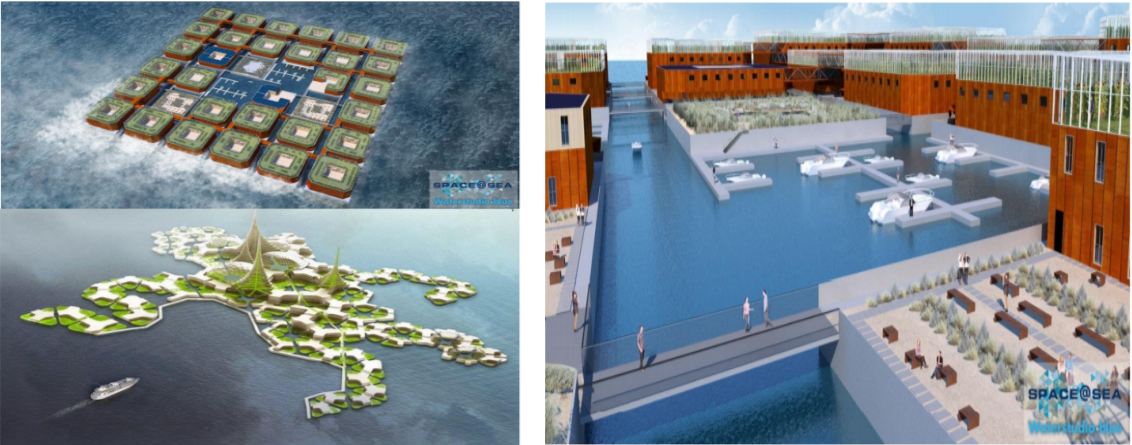
\includegraphics[width=\linewidth]{figures/Literature_Introduction/space@sea_renders.PNG}
    \caption{Living@Sea rendering for Space@Sea \parencite{businessCase_S@S_D1.1}}
    \label{fig:my_label}
\end{figure}

The feasibility of floating islands is analysed in the 3-year project Space@Sea, whose main statement is; "Seventeen European partners aim to provide a sustainable and affordable workspace at sea by developing a standardised and cost-efficient modular island with low ecological impact" \parencite{businessCase_S@S_D1.1}. This study was carried out for two different cases, where the first was located in the Mediterranean Sea, while the other was situated in the North Sea. The Mediterranean business case evaluated \acrshort{capex} (\acrlong{capex}: Major purchases that are designed to be used over the long term) are 49\% and \acrshort{opex} (\acrlong{opex}: Day-to-day expenses) are 99\% of its alternative: the fixed jacket. This difference in \acrshort{capex} is due to the deep water characteristics of the Mediterranean, where a soft mooring system (of a floating island) would be much cheaper instead of jackets fixed to the bottom of the sea. The alternative in the North Sea was land reclamation, which is possible here due to the low water depth. Therefore, the costs of a floating island were compared to the costs of constructing an island by land reclamation in the North Sea business case. The \acrshort{capex} of a floating island would be 183\% and its \acrshort{opex} 138\% of the \acrshort{capex} and \acrshort{opex} of its competitor, due to the high costs of the current design of the mooring system. Due to the geographical position of the floating island, the northern swell in the North Sea can deliver waves with a wave height of up to nine metres, resulting in high \acrshort{capex} (owing to high mooring costs) and \acrshort{opex} (due to maintenance of the modules and connectors). The wave height is determined by the wind, the distance from the upwind coastline (\textit{fetch}) and the time since the wind started blowing \parencite{Holthuijsen2007}. The location studied in the North Sea is at 51$\deg$ N, 3$\deg$ S (see the green mark in Figure \ref{fig:locationNS}), so when the wind comes from the north-northwest, the fetch reaches all the way up to the Arctic Sea, resulting in waves coming from this direction that can get immense under certain conditions.

\begin{figure}[H]
    \centering
    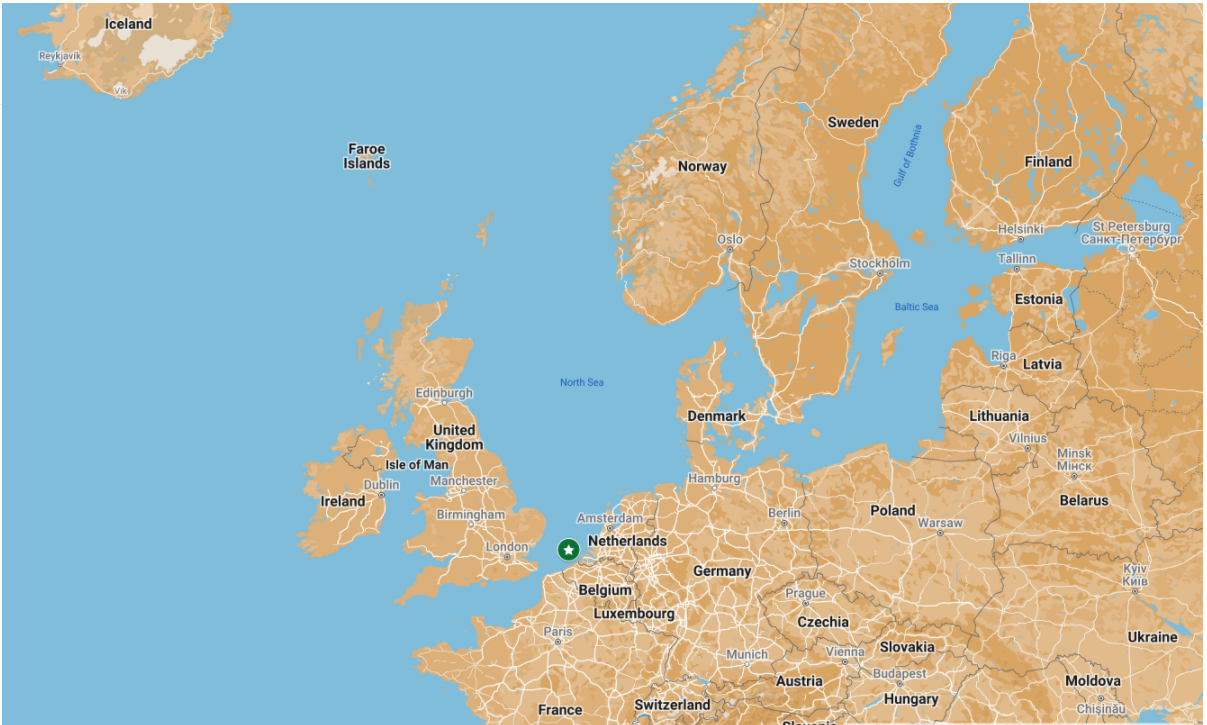
\includegraphics[width=1\linewidth]{figures/Literature_Introduction/location_NS.PNG}
    \caption{Location floating island North sea}
    \label{fig:locationNS}
\end{figure}

Breakwaters, connected to the wave-ward side of floating islands, can provide shelter by attenuating waves through dissipation and reflection. Therefore, they contribute to increasing the number of possible locations where such a floating island could function in the future. Many studies have been conducted on the topic of breakwaters (which are addressed in Chapter \ref{ch:literaturereview}), yet never with a connection to a large structure such as a floating island in this case. \\
\\
Furthermore, there is a knowledge gap in using design optimisation with ComFLOW in combination with the study of breakwaters, and the validation of ComFLOW's results regarding the mean wave drift force on box-type breakwaters interacting with regular waves has not been executed before. 


\section{Problem statement}
Wave drift forces are a consequence of wave loads. These forces cause the floating structure, when freely floating in waves, to drift in the direction of propagation of the waves due to the second-order wave forces \parencite{journee2000offshore}. The mooring system is there to provide the counter force to keep the structure in its place. When the mean wave drift force on the structure increases, its required mooring system becomes more expensive. The magnitude of these second-order wave drift forces scales quadratically to the height of the waves. Therefore, the mooring costs are highly dependent on the height of the incoming waves.\\
\\
% Furthermore, the individual modules of a floating island will move with respect to each other under the action of waves. The fenders (connectors between the different modules) are designed to keep the modules together as one floating structure and will therefore need to withstand loads. The higher these loads are, the more robust and expensive the fenders need to be. So, also the fender costs are dependent on the height of the waves interacting with the structure.\\
% \\



Therefore, to make floating islands an applicable option to provide living/working spaces at sea, the energy of the waves must be dissipated and reflected with the help of a breakwater with an optimised geometry. Research questions are being developed from which thorough research is needed to answer them. This is then required to achieve this objective.

% Because both the construction and maintenance costs of the floating island depend strongly on the height of the waves interacting with the structure, it is economically beneficial to come up with way to attenuate the incoming waves. A breakwater can serve this purpose by dissipating and reflecting wave energy. 


\section{Research questions}
\label{sec: research questions}
The main objective is to attenuate the waves that interact with the structure and thus lower the drift forces and the hydroelastic response of the floating island. Lowering the drift forces will lead to a reduction in the mooring costs, and lowering the motions of the individual modules will lead to an increase in the workability of the island. Due to the infinite number of possible geometries of the floating breakwater and the various external conditions in which it must operate, the optimisation's \textit{design space} is large. Therefore, optimisation will be used to come up with a final design. This main objective is formulated as a question and therefore is the main research question for this thesis: 

\begin{enumerate}
    \item How can the construction costs of a floating island be reduced by connecting a structure to its wave-ward side with an optimised geometry?
\end{enumerate}


The sub-research questions are formulated as follows:
\begin{enumerate}[resume]
    \item What is the quality of the results of ComFLOW with the best possible settings?
    \item How do wave attenuation and reduction of drift forces relate to the geometry of the breakwater?
    \item How are the drift forces and the geometry of the breakwater quantified in mooring and construction costs, respectively?
\end{enumerate}





%\section{Research approach}

% -right grid 
% -validation ComFLOW, reflection and dissipation


% -optimisation between ComFLOW and optimisation method, which is considering the which evaluations to compute

% -design of experiments



\section{Report structure}
This report is structured as follows:


\begin{itemize}
    \item In Chapter \ref{ch:literaturereview} a review of the literature can be found on the studies of floating islands, floating breakwaters, wave forces on marine structures, optimisation techniques and \acrfull{cfd}, with ComFLOW in particular. 
    \item Chapter \ref{ch: methodolgy} describes extensively the methodology of this thesis, with the setup of the optimisation, the post-processing of ComFLOW results and the cost function which calculates the cost reduction each breakwater delivers.
    \item In Chapter \ref{ch: validation comflow} the validation of ComFLOW is discussed. This resulted in certain settings and a grid. Also, a comparison is made with the results of ComFLOW with linear wave theory and an experiment in which waves plunged over a breaker bar. 
    \item An hydrodynamic design optimisation is given in Chapter \ref{ch: captive design optimisation}, where the link is made between the geometry of the breakwater and its hydrodynamic performance. 
    \item An economic design optimisation is given in Chapter \ref{ch: economical design optimisation } to obtain the optimal geometry of the breakwater regarding the reduction in capital expenditure.
    \item Finally, the conclusions and recommendations are presented in Chapter \ref{ch: conclusions recommendations}.
\end{itemize}



\chapter{Literature Review}
\label{ch:literaturereview}


% \begin{figure}
%     \centering
%     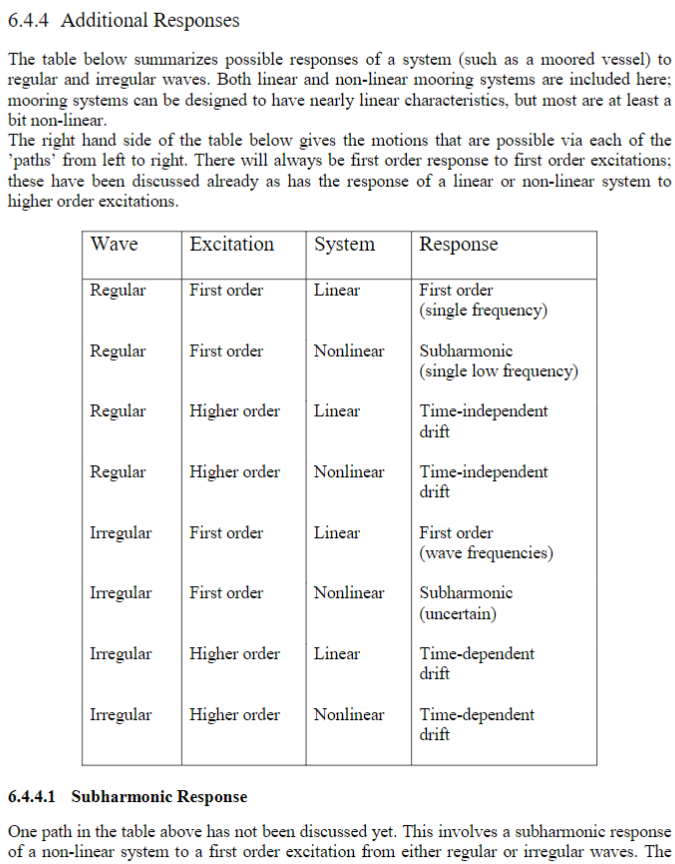
\includegraphics[width=\linewidth]{figures/Literature_Introduction/to_discuss_book_offshorehydromechanics.PNG}
%     \caption{Caption}
%     \label{fig:my_label}
% \end{figure}

% \begin{figure}
%     \centering
%     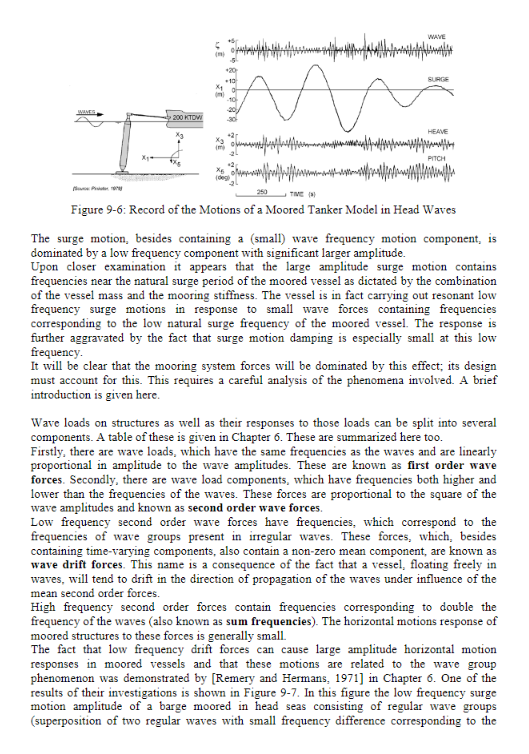
\includegraphics[width=\linewidth]{figures/Literature_Introduction/to_discuss2_book_offshorehydromechanics.PNG}
%     \caption{Caption}
%     \label{fig:largeexcitation_lowfreq}
% \end{figure}


\label{ch: background and literature}


%%%%%%%%%%%%%%%%%%%%%%%%%%%%%%%%%%%%%%%%%%%%%%%%%%%%%%%%%%%%%%%%%%%%%%%%%%
\section{Studies of floating islands}
\label{sec: floating islands}
%%%%%%%%%%%%%%%%%%%%%%%%%%%%%%%%%%%%%%%%%%%%%%%%%%%%%%%%%%%%%%%%%%%%%%%%%%

% \parencite{Waals2018}:\\
% Model tests are done for a floating mega island in large waves up to 15.5 m Hs. Motions are studied. Also numerical calculations are done, but without the connections between the modules. Large mooring forces are found at the natural surge frezuency of the modules. In the third wave, there is a response peak at approximately two times the frequency of wave peak period. This third response is not fully understood. Sum frequent second order drift forces might be an explanation. Differences between the numerical model and experimental model tests were large.\\
% \\

% \parencite{Otto2019}:\\
% Positive drift forces are found for single triangular body. This means the body will drift towards the waves. This is due to the potential solver which takes no radiation damping and viscous damping into account. \\
% \\
% At the frequencies with the largest motion response, the wave excitation at the leeward modules is close to zero as the waveward islands diffract the incoming wave. \\
% At slightly lower frequencies there is however motion response of the leeward islands, despite that there is no wave excitation acting on them. They are responding to the radiated waves of the waveward triangles.  \\
% For the higher frequencies the interference patterns result in wave excitation on both the waveward and leeward triangles. The motion response on this excitation is however small due to the inertia of the triangles.\\

% \parencite{Isope2019}:\\
% In \parencite{Isope2019}, design  optimisations  have  been performed by  varying  the draught, size and shape of the islands, making use of the numerical procedure as described in Otto (2019).


Floating mega-islands can provide an attractive solution for creating more space in coastal areas with the high demand for real estate and the probability that less land will be available in the future due to the rising sea level. They can also serve as a central point where large merchant vessels can unload their cargo without manoeuvring into an inland harbour \parencite{businessCase_S@S_D1.1}.\\
\\
Experimental and numerical tests have been performed to study the wave-induced motions of a floating island. A piecewise flexible island has been model tested at MARIN as described in \citet{Waals2018}, where the motion behaviour was investigated under the action of waves. Furthermore, the mooring loads and connector loads were analysed in mild and severe sea states. In \parencite{Otto2019}, experimental results and numerical simulations have been compared to describe the behaviour of motion. In \parencite{Isope2019}, the same numerical method was used to make design optimisations by varying the draught, size and shape of the islands. The latter three studies selected triangular-shaped modules to restrict the least degrees of freedom of motion possible for each floater \parencite{Waals2018}. A project partly funded by the European Union called Space@Sea also conducted an extensive case study on the feasibility of multi-use modular floating islands. This case study has been very extensive, covering all fields necessary to realise functioning floating islands in the open sea. For this master thesis, only the results concerning the hydrodynamic performance will be analysed. Space@Sea made the switch from triangular-shaped modules to square shapes from practical points of view. Square modules are cheaper in manufacturing and can be used more efficiently in urban planning \parencite{S@SInventoryRegulations}.  \\
\\



The studies mentioned above concluded what the most important hydrodynamic challenges of realising floating islands are:
\begin{enumerate}
    \item Reducing second-order wave drift forces acting on a floating island.
    \item The reduction in the hydroelastic response of a floating island: first-order motions of the modules are unfavourable for the workability/liveability of the floating island, and they result in high connector loads. 
\end{enumerate}


When a floating structure is placed in the sea, it will experience motions as a result of the action of the waves. To avoid large motions, very large structures are desired when these structures need to serve as living and working spaces for people. But large structures experience large drift forces due to second-order wave forces, which will cause low-frequent high-amplitude motions (see Figure \ref{fig: low freq surge motions}). A mooring system, consisting of several lines connected to the sea bottom, will prevent the floating island from floating away (see the Figure below). 
\begin{figure}[H]
    \centering
    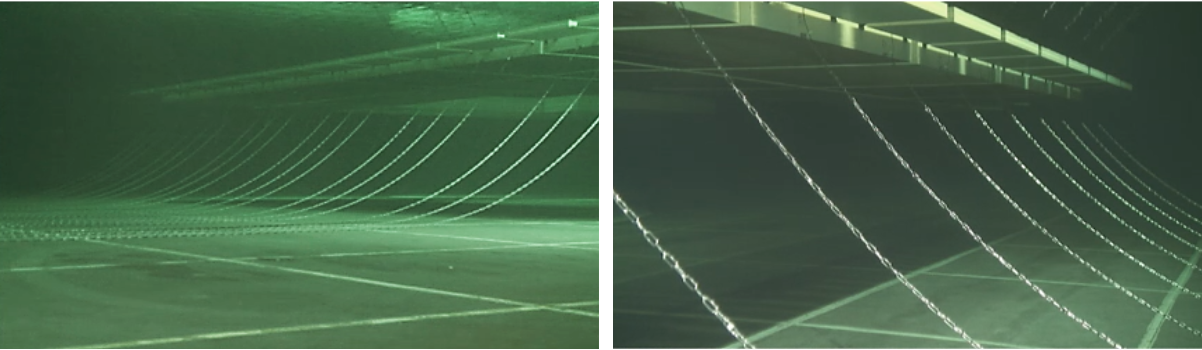
\includegraphics[width=\linewidth]{figures/Literature_Introduction/mooringlines.PNG}
    \caption{Mooring lines of model test \parencite{S@S_demonstationatwavetank}}
    \label{fig:mooringlines}
\end{figure}

Due to the catenary effect, a restoring force is created, which allows the structure to drift in these low-frequent and high-amplitude motions, while the weight of the cables will restore the floating island into its mean position. These motions are allowed up to the point that the mooring lines are taut, so the elasticity of the system depends on the amount of slack that can be applied to the lines. When a floating island is placed in deeper water, more slack can be achieved without touching the bottom much. In shallow water, the mooring system needs to be more complex to achieve the same effect. The floating islands' alternative: land reclamation, is less expensive in shallow water as well. In other words, the local water depth is a limiting factor in the feasibility of a floating island. Due to this phenomenon, a conclusion drawn from Space@Sea was that a floating island placed in the Mediterranean Sea is cost-effective, but not in the North Sea \parencite{businessCase_S@S_D1.1}. 



However, Space@Sea did not perform extensive research on the possibilities of floating breakwaters. Floating breakwaters can broaden the window of geographical locations in which a functional floating island is possible, by lowering the drift forces acting on the floating island. The processes that take place in these drift forces are elaborated more in appendix \ref{appendix:derivation 2nd order wave force}.\\
\\
 
\begin{figure}
    \centering
    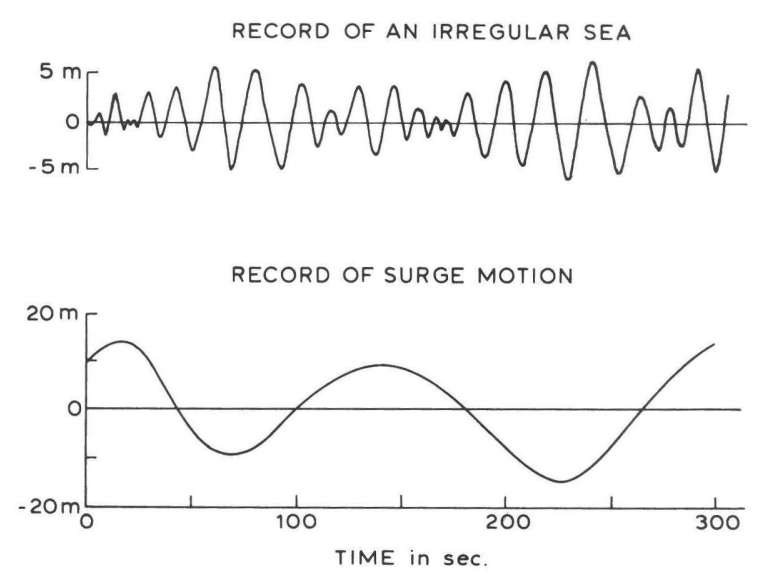
\includegraphics[width=0.7\linewidth]{figures/Literature_Introduction/large_amplitude_low_freq_motions.PNG}
    \caption{Low-frequency surge motions of a moored LNG carrier in irregular head seas \parencite{Pinkster1980}}
    \label{fig: low freq surge motions}
\end{figure}



While incident waves at a large floating structure result in wave drift forces, they will also move the structure in higher frequent motions in other degrees of freedom. These motions result in high loads on the connectors of the modules \parencite{Isope2019}. This effect is another limiting factor in which a floating island can function until the connector forces are unbearable. Of course, the reduction of both the drift forces and motions goes hand in hand, since attenuating the waves will help against both phenomena. But there is a difference in how attenuation needs to be handled, this is clarified in more detail in Section \ref{sec: floating breakwaters}.

%It should be noted that the relative importance of the drift force increases with increasing wave height as it is quadratic in wave height \parencite{Isope2019}. 






% \textbf{todo:} QTF  scales quadratically with the height of the waves! look at Pinkster 1980!, therefore there is a point in which the motions of the island are THE limiting factor OR the drift forces.


%%%%%%%%%%%%%%%%%%%%%%%%%%%%%%%%%%%%%%%%%%%%%%%%%%%%%%%%%%%%%%%%%%%%%%%%%%
\section{Floating breakwaters}
\label{sec: floating breakwaters}
%%%%%%%%%%%%%%%%%%%%%%%%%%%%%%%%%%%%%%%%%%%%%%%%%%%%%%%%%%%%%%%%%%%%%%%%%%

Floating breakwaters have been investigated for a long time. More than 60 configurations of floating breakwaters were recognized by \parencite{jones1971transportable} and \parencite{richey1974floating}. Later, \parencite{Hales1981} separated them into 11 different categories based on their fundamental characteristics. \parencite{McCartney1985} chose to subdivide them into four general categories: box, pontoon, mat, and tethered float, and reviewed them based on their performance in reducing wave height and evaluated their construction costs. \parencite{Sawaragi1995} classified the floating breakwaters into 3 groups: reflection type, reflection and wave breaking type and friction type. Recently, \parencite{Dai2018} did an extensive review on recent research and developments on floating breakwaters, where the different types of floating breakwater were classified into (1) box type, (2) pontoon type, (3) frame type, (4) mat type, (5) tethered float type, (6) horizontal plate type, and (7) other types. However, most of the studies have been done in intermediate to shallow waters (e.g. for the protection of harbours). These floating breakwaters play an important role in providing shelter against wave action by attenuating the energy of incident waves through reflection and/or dissipation. The floating breakwater that was spectacular in terms of its performance is the one in Monaco; it was designed to attenuate 80\% of the wave energy with 2.8 m of significant wave height and 7.2 s of peak period \parencite{Ruggeri2017}. The most common is the box-type floating breakwater, which consists of a solid box that floats on the water surface \parencite{McCartney1985}. An empirical formula for this kind of breakwater has been formulated by \parencite{macagno1953fluid}, where the box is not moving, 2D conditions are assumed, and dissipation is neglected:

\begin{equation}
    K_{\mathrm{t}}=\frac{1}{\sqrt{1+\left[\frac{k W_{\mathrm{f}} \sinh (k h)}{2 \cosh \left(k h-k T_{\mathrm{f}}\right)}\right]^{2}}}
    \label{eq: macagno1953}
\end{equation}
Here, the wave transmission coefficient $K_t$ is expressed as a function of the water depth $h$, the floater width $W_f$, and draught $T_f$.\\
\\

Since conventional bottom-fixed breakwaters can reflect 100\% of incident wave energy, they are most effective in mitigating the hydroelastic response on the floating island. But when the depth of the water increases, its costs will become enormous. A significant reduction could also be obtained by using floating-type breakwaters, provided that the draught of the breakwater and the width to wavelength ratio are sufficiently large \parencite{Wang2010}. Floating breakwaters are preferred compared to bottom fixed breakwaters in the conditions where
\begin{enumerate}
    \item the bottom does not support bottom-founded breakwaters
    \item the water depth is too large such that bottom-founded breakwaters are too expensive
    \item the water quality has to be sustained due to minimal interference with water circulation and fish migration.
    \item good aesthetics are desired; floating breakwaters have a low profile and present a minimum intrusion on the horizon, particularly for areas with high tide ranges.
    \item a temporary breakwater is desired. 
\end{enumerate}


The main purpose and, therefore, the main research objective of this thesis is more nuanced than attenuating waves alone. In this research, the best design of a floating breakwater is studied to reduce the drift forces and motions of a floating island connected to its lee side. It is proven that reflecting wave energy can have a reduction in the motions of the floating island but will only result in higher drift forces acting on the floating breakwater. Accordingly, it is more beneficial to dissipate the waves than to reflect them. The derivation of this proof is shown in Appendix \ref{appendix:reflectionversusdrift}.
\\


\subsection{Wave forces on marine structures}
The wave forces acting on marine structures have been extensively studied. \parencite{Maruo1960} presented a hydrodynamic theory of the drifting force acting on a circular cylinder, a sphere, and other simple solids on a water wave. It was stated that the two-dimensional case of an infinitely long cylinder floating in regular waves with its axis perpendicular to the wave direction has a mean wave drift force of:
\begin{equation}
    \Bar{F} = \frac{1}{8}\rho g H_i^2
\end{equation}

\parencite{longuethiggins1977} derived an expression for the mean wave drift force as a function of the incident, reflected, and transmitted wave height:
\begin{equation}
    \Bar{F} = \frac{1}{16}\rho g (H_i^2 + H_r^2 - H_t^2)(1 + \frac{2kh}{sinh(2kh)})
    \label{eq: longuethiggins force}
\end{equation}
Where incident, reflected and transmitted wave heights are shown as, respectively $H_i$, $H_r$ and $H_t$, the wave number as $k$ and the water depth as $h$.\\
\\
Also, \parencite{longuethiggins1977} confirmed that the mean force on submerged bodies is sometimes reduced and even reversed. An explanation is suggested in terms of the "wave setup" produced by breaking waves.\\
\\

Wave loads on structures and their responses can be split into several components, which is discussed extensively in the doctor's thesis of \parencite{Pinkster1980} and later summarized in \parencite{journee2000offshore}. They are also shown in the following content.
First, wave loads that have the same frequencies as the waves and are linearly proportional to the amplitude of those waves are known as \textbf{first order wave forces}. Second, there are wave force components with a frequency higher than or lower than the wave frequency; they are called \textbf{second order wave forces}. 
Second-order low-frequency wave forces have frequencies, which correspond to the frequencies of wave groups present in irregular waves. These forces contain a time-dependent part, but also have a non-zero mean, which is called \textbf{mean wave drift force}.
The second-order high-frequency wave forces contain frequencies that are twice the frequency of the waves, and they are called \textbf{sum frequencies}. The horizontal response of large moored structures to these forces is generally small. The Table below summarises the possible responses of a system to regular and irregular waves. 

\begin{table}
\centering
\begin{tabular}{|l|l|l|l|} 
\hline
\textbf{Wave}      & \textbf{Excitation}   & \textbf{System}    & \textbf{Response}                            \\ 
\hhline{|====|}
Regular   & First order  & Linear    & First order~(single frequency)      \\ 
\hline
Regular   & First order  & Nonlinear & Subharmonic~(single low frequency)  \\ 
\hline
Regular   & Higher order & Linear    & Time-independent~drift              \\ 
\hline
Regular   & Higher order & Nonlinear & Time-independent~drift              \\ 
\hline
Irregular & First order  & Linear    & First order (wave frequencies)      \\ 
\hline
Irregular & First order  & Nonlinear & Subharmonic (uncertain)             \\ 
\hline
Irregular & Higher order & Linear    & Time-dependent~drift                \\ 
\hline
Irregular & Higher order & Nonlinear & Time-dependent~drift                \\
\hline
\end{tabular}
\caption{Possible responses of a structure under the action of waves \parencite{journee2000offshore}}
\end{table} 



% \subsection{Wave breaking}
% \label{sec: literature wave breaking}
% -Iribarren\\
% -splunging, spilling and collapsing dependent on iribarren\\
% -is er al onderzoek gedaan naar hoeveelheid dissipatie van allen (wel meeste reflectie bij grote slope though)?\\





% The amount of studies that have been done in the field of floating breakwaters is tremendous. But with the knowledge gained that the wave attenuation is best obtained from viscous dissipation and the floating breakwater is going to be connected to the floating island, the scope of this study is limited much more.  \\
% \\


% \subsection{Useful literature regarding floating breakwaters}
% Although a lot of studies have been done on the topic of floating breakwaters, the choice in setup causes the number of studies which proved to be useful converges drastically. \\
% \\




%many studies have been done, not everything is useful
%focus on dissipative floating breakwaters
%setup is chosen for the floating breakwater connected to the island, to increase stiffness, because this brings a higher potential to absorb wave energy SOURCE.
%pile supported floating breakwaters may be interesting

% \section{Wave conditions}
% \label{sec: wave conditions}
% % -Irregular waves needed for compliance natural frequency of moored structure --> or take regular waves exactly at natural frequency
% % -eventually conclusion of this section has to be: use regular waves, but choose them wisely (simulation time savings)



% %%%%%%%%%%%%%%%%%%%%%%%%%%%%%%%%%%%%%%%%%%%%%%%%%%%
\section{Optimisation techniques}
% %%%%%%%%%%%%%%%%%%%%%%%%%%%%%%%%%%%%%%%%%%%%%%%%%%%




% % %optimize on motions and drift forces 
% % \textbf{todo:} uitvinden of irregular waves/ regular waves het beste is, afhankelijk van rekentijd van simulatie


On the basis of the literature study on floating breakwaters, a design for the breakwater will be made that best suits its application. The exact dimensions of this breakwater depend on various external parameters, like the geometry of the floating island connected to the lee-side of the breakwater, the water depth, the maximum allowable mooring forces, and the wave conditions. Since many different configurations of these parameters are possible, a smart optimisation method is used to design the breakwater. Several optimisation techniques and tools are already existing; one of these tools is Design Expert, which is based on the method: \acrfull{doe} and is explained in Section \ref{sec: DoE}



% \textbf{Gevonden literatuur:}:
% -Aerodynamic shape optimisation using novel optimizer based on machine learning techniques \parencite{Yan2019}.
% CFD and an optimizer are used to come up with new design.
% Within the optimizer, reinforcement learning is applied to extract the optimisation experience from the semi-empirical method DATCOM using deep neural networks. And transfer learning is implemented to reuse the experience as priori knowledge in the CFD-based optimisation by sharing neural network parameters. \\
% \\
% -A machine learning method for the evaluation of hydrodynamic performance of floating breakwaters in waves \parencite{}. 2D simulation for the idealisation of FBs in regular and irregular waves. Hydrodynamic performance is assessed by a machine learning method based on Cuckoo Search-Least Square Support Vector Machine model. Output minimal wave height required.\\
% \\
% \acrfull{MOGA} is one of many engineering optimisation techniques, a guided random search method with the possibility to search a diverse set of solutions with more variables that can be optimized at one time. Solutions are illustrated using Pareto fronts. Compared to the conventional method for solving multi-objective problems, \acrshort{MOGA} takes a relatively short computing time .




% \subsection{Topology optimisation}
% Topology optimisation is well-established tool in computational structural engineering \parencite{bendsoe2003topology}. In its simplest realisation in structural engineering, a topological optimisation starts with a certain domain entirely filled up by solid material of a certain density. Then the loads are applied, where the stresses are least, material is discarded or the density of the material is lowered. Then the stresses will be calculated again under the same loads and the same process repeats itself until a high-density material is left only in regions that are critical to fulfil the structural task, and in this way the optimal lightweight structural design is met \parencite{Othmer2014}. This method came to the field of \acrfull{cfd} in 2003, where \parencite{borrvall2003topology} and \parencite{moos2004bionic} presented independently a way to optimize ducted flows. With a fixed inlet and outlet, the starting point with a big domain. Then they used some local criterion to determine whether an area was counterproductive with respect to the chosen objective and iteratively removed parts from the domain. Until the optimal duct between the inlet en outlet were reached of a given installation space. Topology optimisation is different from \textit{shape optimisation} and \textit{sizing optimisation}, because the design can attain any shape within the design space, instead of dealing with predefined configurations. \\
% \\
% Topology optimisation for fluid-structure interaction problems have been studied in \parencite{}, \parencite{}, \parencite{} and \parencite{}. 





% % % \subsection{Definition Machine Learning}
% % % Building models from data with optimisation and regression


% \subsection{DAKOTA}
% \label{sec: dakota}
% Dakota (Design and Analysis Toolkit for optimisation and Terascale Applications) is going to be the interface between the simulation code ComFLOW and the iterative analysis method. Dakota contains algorithms for optimisation with gradient and non gradient-based methods; uncertainty quantifications with sampling, reliability, and stochastic expansion methods; parameter estimation with nonlinear least squares methods; and sensitivity/variance analysis with design of experiments and parameter study methods. By employing object-oriented design to implement abstractions of the key components required for iterative system analysis, the Dakota toolkit provides a flexible and extensible problem-solving environment for the design and performance analysis of computational models on high-performance computers \parencite{DakotaManual2021}. \\
% \\
% Dakota provides several capabilities:
% \begin{itemize}
%     \item \textbf{MOGA} (described in section 6.2.3.1 of \parencite{DakotaManual2021})
%     \item \textbf{Pareto-set strategy} (described in section 14.4 of \parencite{DakotaManual2021})
%     \item \textbf{Weighting factor approach for multiobjective reduction:} a composite objective function is constructed from a set of individual objective functions using a user-specified set of weighting factors.
% \end{itemize}

% In engineering, a design tool by combining a \acrfull{cfd} solver and DAKOTA is already developed with the design of wind turbine blades \parencite{Quan2020}, helicopter rotor blades \parencite{Leusink2015}, barriers for windblown sand mitigation \parencite{Horvat2020} and squirrel cage fans \parencite{Hocine2021}. The drawback of using a \acrfull{GA} is that it requires a high number of evaluations. This is acceptable for industrial applications when using a low time-consuming \acrshort{cfd} solver, but leads to unreasonable high computational costs when a high fidelity \acrshort{cfd} tool is used. 


% % % \textbf{todo:} hoge snelheden leiden tot kleine tijdsstap (motivatie om enkel de FB te modelleren)


\subsection{\acrfull{doe}}
\label{sec: DoE}
Experimentation is used to find the best result or the final design in all kinds of fields. Think, e.g., of construction, biology, education, communication, science, and art. But mostly it is a costly and time-consuming process. When striving for efficiency, is there a way to streamline the work process to get more learning with less experimentation? Here, \acrfull{doe} comes into play. \acrshort{doe} is a systematic and efficient method that allows scientists and engineers to study the relationship between multiple input variables and key output variables. In short, it can optimise the experimentation process by predicting the trend between the change in input variables on the change in the output of the system. \acrshort{doe} is convenient to use:
\begin{itemize}
    \item To determine whether an input variable affects an output variable
    \item To determine whether input variables interact with the output variable
    \item To model the behaviour of the output variables as a function of input variables
    \item To optimize the output variables
\end{itemize}

%The way to implement \acrshort{doe} is as follows. First, the goal of the experiment is determined, from which a response (a result which you can measure well and has influence on the eventual goal) is obtained. Secondly, constant and variable factors are included. The shape and magnitude of the variable factors will affect the response. Next, a model is included which adequately describes the physical situation. Now, all the input is used to generate a design with \acrshort{doe}. 

Different publications that did a \acrshort{doe} optimisation were reviewed by \citet{Weissman2015}, who found that the application of \acrshort{doe} to the development of pharmaceutical processes has increased greatly over the past 11 years. This paper also summarised several steps on how to implement \acrshort{doe} as follows:

\begin{enumerate}
    \item Define the Objective: What problem needs to be resolved? Frequently, the goal is to optimise a design, but sometimes the design conditions are "locked," and the goal is merely to understand the robustness of the existing conditions. In this case, robustness is defined as probing the impact (if any) of small changes in the continuous factors on the outcome.
    
    \item Define Factors/Variables and Their Ranges: The determination of which factors / variables are included in a \acrshort{doe} depends on the resources. More variables will lead to more evaluations. Therefore, it is imperative to prioritise them, using existing knowledge, into groups that are known to be impactful, suspected, possible, and unlikely. Then, assign high and low settings to the factors selected for inclusion in the study, as is the case when using the common two-level factorial design. These settings must be relevant, achievable, and practical. The end product of this exercise is the creation of \textit{design space}.
    
    \item Define the Responses: These are the measurable outcomes of the process. Responses are related to the objectives. 
    
    \item Select the Experimental Design: The choice depends on the objective, the number of factors, and the available resources. The most common are screening designs in which qualitative information about the relevant factors is obtained. These designs also allow the factors to be ranked in the order in which they impact the response. Screening designs are frequently used to filter irrelevant factors to enable focus on the most relevant factors in a second \acrshort{doe} design, also known as optimisation designs. These latter designs require more experiments than screening designs but generate a more comprehensive model of the response surface. 
    
    \item Generate Reaction Worksheet: The input of all the above information into the software will generate a list of configurations to perform.

\end{enumerate}
%more steps are shown in the paper! but this may be complete for me already.

\acrshort{doe} in combination with \acrshort{cfd} is used earlier in optimising the cooling fan performance by \citet{Hagenmaier2002} and in designing an optimal scram jet by \citet{Srinivasa2014}. The use of \acrshort{doe} and \acrshort{cfd} in the study for the optimal breakwater design has not been done before.



% - trial-and-error method and one factor at a time


% \subsection{Multi-fidelity optimisation}
% % %auke van der ploeg vertelde hierover
% % -definitie

% To speed up the optimisation process, the multi-fidelity approach can be used. Here the largest part of the optimisation is carried out by using a coarser grid, from which the results are refined progressively by increasing the resolution of the design domain. In other words, by incorporating low-fidelity data, the feasibility constraints can be modelled accurately using only a small number of high-fidelity evaluations on the feasibility boundary. This has been done for the aerodynamic design of helicopter blades by \citet{Leusink2015} and in wind farm framework optimisation by \citet{multifidelity_windfarm}

% % -voorbeelden van papers die dit gebruiken (https://onlinelibrary.wiley.com/doi/epdf/10.1002/we.1667) (check wikipedia voor meer onderzoeken)



% %%%%%%%%%%%%%%%%%%%%%%%%%%%%%%%%%%%%%%%%%%%%%%%%%%%

\section{\acrfull{cfd}}
In the field of \acrfull{cfd}, often one or a combination of the following equations is being modeled \parencite{vanderPlas2017}:
\begin{itemize}
    \item Navier-Stokes equations (viscous flow)
    \item Euler equations (non-viscous flow) 
    \item potential equations (non-viscous, irrotational flow)
\end{itemize}
These three methods are by no means comprehensive. For most applications, \acrfull{DNS} of the Navier-Stokes equations is too expensive. With a \acrshort{DNS}, the entire range of spatial and temporal scales of turbulence is resolved; from the smallest dissipative scales (Kolmogorov microscales) to the integral length scale $L$ of the motions where most of the kinetic energy is located \parencite{Westerweel_Turbulence2016}. A so-called turbulence model can be implemented to save computational time. This is a simplification of the Navier-Stokes equation, a mathematical model in which the effects of turbulence are predicted. 
In the particular field of wave modelling, other techniques are used, such as wave theory or the modelling of, for example, the Boussinesq equations \parencite{vanderPlas2017}.\\
\\
In the field of \acrshort{cfd}, a commonly encountered field of engineering application involves modelling of wave impact on an offshore structure. If the geometry is not too complicated, it is still possible to use potential theory in combination with empirical formulae with the prediction of impact forces. To obtain flow around very complicated structures, these formulae do not comply with reality, so \acrshort{DNS} is required.

\subsection{ComFLOW}
\label{subsec: comflow literature review}
%  \textcolor{red}{\textbf{todo: include: Low-order not a problem because cells and time steps need to be small anyway, because of large gradients and discontinuities near the free surface}}\\
%  \\
With exactly this field in mind, a \acrshort{cfd} solver is developed: ComFLOW, which describes the motion of an incompressible viscous fluid. Examples of ComFLOW's applications are as follows:
\begin{itemize}
    \item wave impacts
    \item green water loading on ships
    \item liquid sloshing in LNG carriers
\end{itemize}

The solver has its roots in simulating the liquid sloshing on board spacecraft \parencite{veldman1984axisymmetric}. For this application, it was developed for microgravity conditions, where surface tension played a dominant role. At Deltares Research Institute, the code was extended to enable simulation of wave impacts. In the 1990s, ComFLOW found its applications in offshore structures, when fully 3D flow around complex geometries could be simulated. Furthermore, the latest developments concentrated on free-surface simulation, wave propagation, wave impact simulation, and the addition of a two-phase flow model \parencite{Kleefsman2005}, \parencite{Wemmenhove2008}. \\
\\
In this master thesis, the hydrodynamic performance of a floating breakwater is investigated. This performance is expressed by the forces acting on the breakwater and its wave attenuating performance. Due to its interaction with breaking waves, where a two-phase flow model of water and air will occur, ComFLOW is selected as a good fit as the \acrshort{cfd} simulation method. \\
\\
Since dissipation is of great importance in this Master's thesis, it is good to mention how ComFLOW handles wave energy dissipation by wave breaking. In ComFLOW, an energy-preserving turbulence model is implemented, which gives an accurate description of large-scale flow effects. However, small-scale production is controlled by a special treatment of the convection term, instead of adding eddy-viscosity \parencite{Luppes2013}. In other words, the physical dissipation in ComFLOW is expected to depend on the size of the grid at the location where wave breaking occurs. \\
\\

ComFLOW has been used before for several applications in the interaction between fluids and structures. A validation of wave run-up calculation methods for a gravity-based structure is done in \citet{Danmeier2008}, sloshing dynamics in LNG tanks was studied by \citet{Wemmenhove2009}, wave-in-deck load on a jacket platform by \citet{Iwanowski2009}, a validation is done by studying ComFLOW performance with wave impacts on a dike by \citet{Wenneker2010}, extreme wave impact on offshore platforms and coastal constructions has been investigated by \citet{Luppes2011}, and recently a shallow water \acrfull{calm} buoy in extreme waves is validated by \citet{Bandringa2021}. 



\section{Scope}
In order to ensure that ComFLOW's results can be used in judging the performance of the breakwaters, it is necessary to study compliance with the reality. Therefore, it is chosen to perform a thorough validation of this \acrshort{cfd} code when waves are interacting with a breakwater. The implementation of this validation in the research questions (see research question 2 in Section \ref{sec: research questions}) shows its prominent role in this thesis. Since wave energy dissipation, reflection and transmission are the most important phenomena to track the performance of breakwaters, these are the parameters were the validation will be based on. \\
\\

% A study to the performance on floating breakwaters with ComFLOW has not been executed before. Therefore, it is chosen to do an extensive validation to this \acrshort{cfd} code when waves are interacting with a breakwater. The implementation of this validation in the research questions (see research question 2 in Section \ref{sec: research questions}) shows its prominent role in this thesis. Since wave energy dissipation, reflection and transmission are the most important phenomena to track the performance of breakwaters, these are the parameters were the validation will be based on. \\
% \\
Increasing the feasibility of floating islands with the help of breakwaters is a new field of research. Therefore, questions need to be answered as: What are the dimensions, shape, and operational water depth of the optimal breakwater in this application for specific wave conditions? A design optimisation, where multiple geometries of breakwaters are going to be evaluated, seems suited well in order to answer these questions. How this is implemented exactly is elaborated more in the following chapter.


\chapter{Methodology}
\label{ch: methodolgy}

% \textbf{todo: keuze bolling ipv holling toelichten}
The objective of this thesis is to increase the feasibility of a floating island by using a structure that attenuates the wave energy. The procedure to achieve this objective is to optimise the design of such a structure with the \acrfull{cfd} program ComFLOW and the design method: \acrfull{doe}. In this section, a methodology is discussed on how this optimisation is going to be realised. \\
\\
The literature review resulted in a scope and some decisions. A fundamental choice about the setup of the breakwater was made quite early in the process, which is discussed in Section \ref{sec: choice setup}. ComFLOW has never been used before to quantify the performance of floating breakwaters. Therefore, the validation in this application seemed crucial. The methodology of this part of the project is reported in Section \ref{sec: methodology validation}. The remaining part of the project consists of the actual optimisation of the breakwater, from which its methodology is described in Section \ref{sec: methodology design optimisation}. \\



\section{Choice in setup: connected to or floating in front the island}
\label{sec: choice setup}
% Floating  breakwaters  are  held  in  place  by  mooring  lines  or  piles,  with  piled  mooring  being  suitable  only at shallow sites (McCartney, 1985).  The mooring lay-out requires careful design to environmental conditions,not only from a structural and mooring integrity point of view, but also because the mooring stiffness affects the attenuation performance of the breakwater (Loukogeorgaki et al., 2017).  A stiffer mooring system tends to lead to better wave attenuation performance (Loukogeorgaki and Angelides, 2005).  Consistently, a captives etup (all degrees of motions restrained) or piled setup (structure can only move vertically) generally induce stronger  wave  attenuation  than  a  moored  setup  (Ruol  et  al.,  2012).   An  exception  is  the  attenuation  at  the wave frequencies corresponding to one of the natural frequencies of the moored floater,  which can be higher for a moored compared to captive setup because of enhanced viscous dissipation induced by resonant motion behaviour  (Ruol  et  al.,  2012;  Ji  et  al.,  2018).   At  the  same  time,  resonant  motion  behaviour  leads  to  high instantaneous mooring loads (Loukogeorgaki and Angelides, 2005) and it is therefore recommended to design the mooring system based on second-order rather than first-order wave excitation (Drimer et al., 1992)


The floating breakwater could be placed a certain distance in front of the floating island (a so-called stand-alone setup), while it is moored by itself and interacts with the waves way before they arrive at the floating island. Or it could be connected to the floating island itself, where it catches the waves just before they can interact with the structure. Both setups have their pros and cons; a stand-alone setup is easier to move and, therefore, widely applicable. But when this breakwater is connected to a floating island, a better wave attenuation performance is expected.\\
\\
Numerical and experimental studies showed that the stiffness of the mooring system of the floating breakwater affects the attenuation of the waves. A stiffer mooring system has a better wave attenuation performance \parencite{Loukogeorgaki2006} \parencite{Loukogeorgaki2017}. A floating breakwater with pile setup, where only a heave motion is allowed, showed better performance than softly moored \parencite{Ruol2012}. Consequently, a fully captive set-up (where all degrees of freedom are restrained) is expected to give the most promising results. This resulted from the experimental study \parencite{Zanden2021}, where a submerged parabolic beach that enforced wave energy dissipation through breaking, was tested both in a soft moored setup and a captive setup. As expected, the captive setup had significantly better wave attenuation performances. The motions of a floating island are naturally much less than those of a smaller stand-alone floating breakwater, so more stiffness can be imposed when the floating breakwater is connected to the structure. This is why the connected setup is expected to have better wave attenuation performances. 
Also, when looking at a stand-alone setup, higher waves will form again on the lee-side of the floating breakwater due to wave diffraction around the structure \parencite{Holthuijsen2007} \parencite{Zanden2021}. In other words, when using the stand-alone setup, which is placed further away from the floating island, the floating breakwater must be wider to achieve the same wave attenuation results. Thus, the choice has been made to make a design of the floating breakwater that is connected to the floating island. \\
\\


\section{Validation}
\label{sec: methodology validation}

The validation of this experiment is done to get used to the software and find the right settings and grid outline, which minimises the computational power required while giving stable simulations and reliable results.\\
\\
When a wave interacts with a breakwater, the wave energy is transmitted through, reflected back, or dissipated at the location of the breakwater. Each of these phenomena was found to be an important quantity to validate in order to judge whether the ComFLOW results are reliable. Wave transmission and forces on the structure will be recorded in ComFLOW simulations with a box-type breakwater, to make a comparison with the analytical formulas: the Macagno formula (equation \ref{eq: macagno1953}) and formula \ref{eq: longuethiggins force} derived by Longuet-Higgins. The Macagno formula predicts wave transmission, and formula \ref{eq: longuethiggins force} describes the forces on a box-type breakwater. Both these formulas are derived from linear wave theory.\\
\\
To track whether ComFLOW handles wave dissipation through wave breaking well and investigate what grid size should be used, a comparison will be made with an experiment in which waves were plunging over a breaker bar for different grid refinements in ComFLOW. The wave transmission after the moment of breaking will be recorded in ComFLOW and compared to the results of the experiment. 



\section{Design optimisation}
\label{sec: methodology design optimisation}
The design optimisation is explained in three different parts: the parametrisation of the breakwater geometry is discussed in \ref{subsec: methodology parametrisation}, the use of \acrfull{doe} in \ref{subsec: methodology doe} and how the simulations need to be handled in ComFLOW in \ref{subsec: methodology comflow}.

\subsection{Parametrisation of breakwater}
\label{subsec: methodology parametrisation}
A floating breakwater must attenuate the wave energy through dissipation and reflection. The literature review in Chapter \ref{ch:literaturereview} showed that a box-type breakwater is capable of reflecting much of the wave energy and an inclined beach under the water surface forces the waves to break and thus dissipate the wave energy. With that in mind, the breakwater is parameterized in such a way that it can take both these forms and many in between. 


\begin{figure}[h]
    \centering
    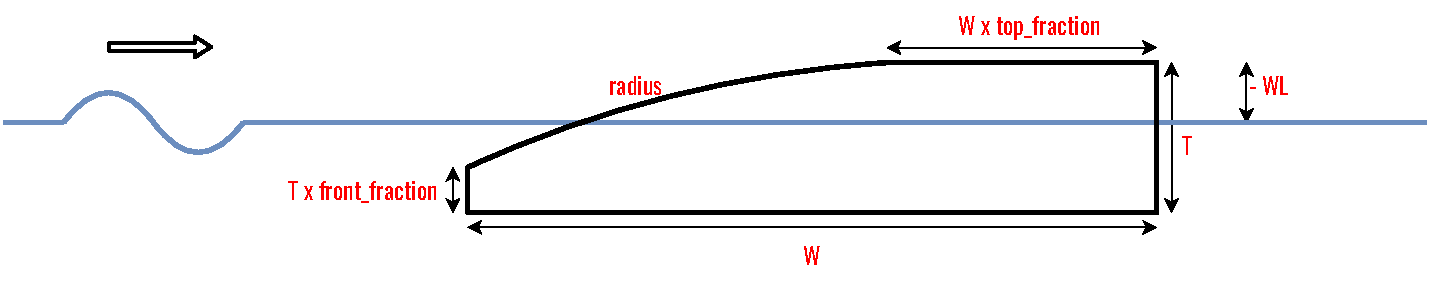
\includegraphics[width = \linewidth]{figures/Methodology/parametrisation.pdf}
    \caption{parametrisation of breakwater}
    \label{fig: parametrisation breakwater}
\end{figure}

The six different parameters (shown in Figure \ref{fig: parametrisation breakwater}) will have the following boundaries, and more elaboration is given below:
\begin{enumerate}
    \item W [m]: dimension in x-direction
    \item T [m]: dimension in z-direction
    \item top\_fraction (0,1): is a fraction of the variable W, such that the length of the top can not exceed the bottom 
    \item front\_fraction (0,1): is a fraction of variable the T, such that the length of the front can not exceed the aft 
    \item radius [m]: the curve of the inclined beach
    \item WL [m]: shift of the water level from the top of the breakwater. 
\end{enumerate}

Here, the fractions (parameters 3 and 4) are values between 0 and 1 so that the front side of the breakwater cannot exceed the depth \textit{T} and the top side cannot exceed the width \textit{W}. The beach is shaped by plotting part of a circle through the locations where the circle crosses the top and the front of the breakwater. The beach curve is varied by changing the radius of this circle (parameter 5). Parameter 6, which defines the z-position of the breakwater, changes the waterline with regard to the origin of the body-fixed coordinate system. For example, with WL = 1 the origin of the body-fixed coordinate system is one metre under the waterline and WL = -1 means that the body-fixed origin is one metre above the waterline.



\subsection{\acrfull{doe}}
\label{subsec: methodology doe}
As discussed extensively in Section \ref{sec: DoE}, \acrshort{doe} is used to make a \textit{design space}, which creates different configurations of the breakwaters, based on the parameters of interest. Then, after the performance of each configuration is quantified using the data from ComFLOW, the dependence of each parameter on the wave attenuation performance and the mean wave drift force can be traced. Then, a sequence of optimal breakwaters will be found ranked according to their desirability.



\subsection{ComFLOW simulations}
\label{subsec: methodology comflow}
ComFLOW will be used to quantify the performance of each configuration. It is investigated how each configuration performs by recording the transmitted wave height and the average surge force on the geometry. These quantities will be translated into a transmission coefficient and a mean wave drift force. 


\subsubsection{Waves}
The design optimisation is done with two different wave conditions, from now on referred to as \textbf{Wave Condition 1} and \textbf{Wave Condition 2}. For both, the characteristics are shown in Table \ref{tab: wave conditions}. Wave Condition 2 is the most extreme wave condition expected to occur in the North Sea in 100 years \citep{Fery2019}. This condition is important to test since the mean wave drift force of the floating island scales with the incoming wave height squared, and so the mooring system needs to be designed for this situation. Its group velocity is 9.69 m/s. Therefore, the first waves arrive at x = 580 m (this is an important position since this is the outer position where the wave height will be recorded; more about this in Section \ref{sec: post processing by Python}) at t = 60 seconds and approximately 23 wave periods will pass until the end of the simulation (t=300 s). To investigate how the optimal breakwater depends on the wave characteristics, the second wave condition is implemented. These waves will arrive at x = 580 m after 120 seconds, and from that moment exactly 30 waves are expected to pass. 

% Please add the following required packages to your document preamble:
% \usepackage{booktabs}
\begin{table}[h]
\begin{tabular}{@{}ccccccccc@{}}
\toprule
Wave Condition & Type    & H {[}m{]} & T {[}s{]} & $\lambda$ {[}m{]} & k {[}m$^{-1}${]} & kh {[}-{]} & c$_p$ {[}m/s{]} & c$_g$ {[}m/s{]} \\ \midrule
1              & Regular & 3.00      & 6.00      & 55.59            & 1.11E-1          & 2.60       & 9.26            & 4.90            \\
2              & Regular & 9.00      & 10.40     & 133.90           & 4.69E-2          & 1.08       & 12.88           & 9.69            \\
 \bottomrule
\end{tabular}
\caption{Two wave conditions used in design optimisation}
\label{tab: wave conditions}
\end{table}


In the simulations, some numerical dissipation causes the actual wave heights, which are interacting with the structure, to be a bit lower. For Wave Condition 2, the actual incident wave height is 2.67 metres, and for Wave Condition 2 it is 8.65 metres.



% \section{parametrisation breakwater}

% \section{Setup simulations}

% -comflow.cfi file with tags, with locations, mass, radius of intertia, attachment point, grid and everything else that is scripted\\
% -stijfheid fenders Table 2-4 van D10.4 S@S:
% \begin{itemize}
%     \item Axial Stiffness = 52.38 MN/m
%     \item Traverse Stiffness = 42.08 MN/m
%     \item Bending Stiffnes = 132.78 MNm/rad
% \end{itemize}
% On S@S project, the 45 m modules had two of these fenders at each side of an island module. So to compute these stiffnesses needed per unit width of breakwater, all the values are multiplied by two and divided by 45. This gives the stiffnesses used in the ComFLOW simulations:
% \begin{itemize}
%     \item Axial Stiffness = 2.33  MN/m
%     \item Traverse Stiffness = 1.87 MN/m
%     \item Bending Stiffnes = 5.90 MNm/rad  * 5 NOTE, FIVE TIMES THE FENDERS
% \end{itemize}

% -z-stijfheid vender:
% \begin{itemize}
%     \item aanname: hydrodynamische stijfheid één eilandmodule W=45, T = 6m
% \end{itemize}


% -check met box onder water of locatie fender goed zit!

% -z-stiffness too stiff. fender s@s/golfhoogte misschien juist (dan met maximale uitslag neemt hij kracht aan van fender stiffness bij 1 m exitatie).



\section{Scripting in Python}
Once a design space is created with the help of \acrshort{doe}, all the different configurations with its parameters are known. Then Python is used to prepare and start all simulations automatically. How this is done is explained in Section \ref{sec: preperation of simulations by Python}. Once the ComFLOW simulations are done, Python is also used to change the raw data into interpretable quantities. How these quantities are exactly calculated out of the raw ComFLOW output is explained in Section \ref{sec: post processing by Python}

\subsection{Preparation of simulations}
\label{sec: preperation of simulations by Python}
\subsubsection{Determining mass, radius of inertia and CoB of geometries}

The mass of each configuration is determined by the volume of the underwater body. To determine this, the body is divided into three areas, denoted by the green numbers in Figure \ref{fig: Figure for mass calculation}. The volume per unit width of area 1 is $W\cdot T\cdot front\_fraction$. The volume per unit width of area 2 is $|x_{WL}|\cdot W\cdot top\_fraction$. The volume per unit width of area 3 is computed numerically with the help of Python. The sloping beach is defined as two arrays, each containing a thousand characters, one defining the beach in z-direction and the other in x-direction. These arrays are used in a for-loop to do the calculation. With the three areas and the location of the waterline known, the total displacement per unit width of the breakwater ($\nabla_{breakwater}$) can be established. Then the mass of the breakwater is nothing less than multiplying that number with the density of the water which is used in ComFLOW: 1000 $kg/m^3$. 

% Symbolically this looks like
% \begin{equation}
%     m_{breakwater}  = \nabla_{breakwater} \cdot \rho_{water}
% \end{equation}
% per unit width of breakwater.\\
% \\

\begin{figure}[h]
    \centering
    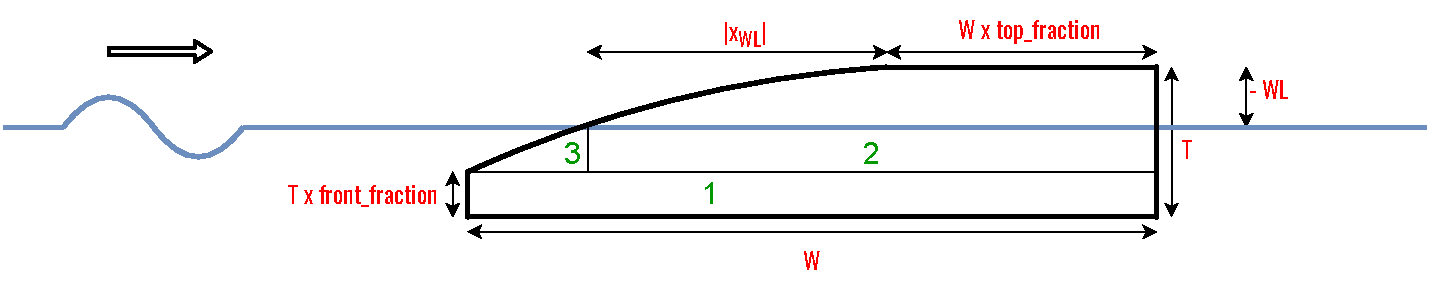
\includegraphics[width=\linewidth]{figures/Methodology/parametrisation_areas.pdf}
    \caption{Division of areas used in calculation of mass breakwater}
    \label{fig: Figure for mass calculation}
\end{figure}

In determining \acrfull{cob} of all geometries, the same division in areas is used. First, the focal point of each area is determined. Area 1 \& 2 both have a very straightforward focal point, and the one of area 3 is again done discretely using Python in the same for-loop as in the calculation of the mass of the breakwater. \\
\\
Since the simulations will be 2D, only pitch rotations occur, so the radius of pitch inertia ($k_{yy}$) must be calculated. For this, the assumption is made that the mass is uniformly distributed over the breakwater. Then the breakwater is divided into finite elements. Each element contributes to the radius of pitch inertia by
\begin{equation}
    k_{yy} = \sqrt{\frac{1}{12}(W^2 + H^2) + d^2}
\end{equation}
where $W$ is the width of that element, $H$ is the height and $d$ is the distance to the \acrfull{cog}. How this is scripted exactly can be seen in Appendix \ref{app: scripts for setting up simulations}.

\subsubsection{Stiffness hinge point with moving breakwaters}
Waves that interact with breakwaters create fluctuations in the pressure around the structure and create motions that the structures in reality have. Therefore, some breakwaters that come out of the optimisation will be resimulated in ComFLOW with an allowance of movement in pitch and surge direction, to map the influence of movements on the results of the optimisation. The presence of a floating island on the lee-side of the breakwater is imitated by defining a hinge point, on the lee-side of the breakwater on the water line (x=450m and z=0m). In 2D simulations, the breakwaters have three degrees of freedom: surge, heave, and pitch. The surge (translation in the x-direction) and the pitch (rotation around the y-axis) with respect to the hinge point will be allowed, and heave is restricted because most of the simulations showed strange unrealistic behaviour of the motions of the breakwaters and eventually caused the simulations to get unstable in most cases. \\
\\
The hinge point is defined in both the body-fixed coordinate system and the general (grid-fixed) coordinate system, and a spring term is imposed between these points. The fenders used for the design of the floating island of Space@Sea have an axial (surge) stiffness of 52.38 MN/m  per fender \citep{S@S_demonstationatwavetank}. Each 45 m wide module had two fenders, so the surge stiffness per unit width of the floating island is ($\frac{52.38 \cdot 45}{2}$) 2.33 MN/m. This value will be used for future simulations. The pitch stiffness of these fenders could not simply be used from the Space@Sea project, because this would cause some breakwaters to resonate in their pitch motion (i.e., their pitch stiffness around the hinge point would coincide with the hinge pitch stiffness). Therefore, the pitch stiffness imposed by the hinge point will be different for each breakwater: 1\% of its own hydrodynamic pitch stiffness with respect to the hinge point. Since there is no restoring moment for completely submerged breakwaters, 1\% of the restoring force of similar breakwater crossing the waterline, with a depth of two meters, is used for the submerged bodies. 




\subsection{Post-processing}
\label{sec: post processing by Python}
ComFLOW gives a raw output that needs to be modified into quantitative parameters to interpret them as perceptible parameters. This section discusses how this is done for the wave transmission of the breakwater and the drift forces on the geometries.



\subsubsection{Mean Wave Drift force}
At each timestamp in ComFLOW, the pressure is determined in each cell, with unit $N/m^2$. To arrive at the force acting on a geometry, the pressure of the cells around the body is integrated. Integrating the pressure in the yz-plane results in a net surge force $F_x$, integrating in the xy-plane in a heave force $F_z$ and for 3D simulations the sway force $F_y$ can be determined by integrating the pressure points in the zy-plane. Since the simulations in this thesis are in two dimensions (x and z), the y-dimension does not exist. Therefore, to obtain the force $F_x$, the pressure left and right of the geometry is integrated in only the dimension z and, therefore, the net resulting force will be a force per unit width of the breakwater, with unit $N/m$.\\
\\
With this in mind, it is understandable that a minimum amount of cells in the z-direction of the body is required to give applicable results for the surge force $F_x$. What this minimum is, is investigated in the validation phase of this thesis and resulted in 20 cells. The smallest dimensions of the cells of the grid around the breakwater are 125 mm. With smaller cells, the time step will be too small, which results in long execution times. Therefore, the minimum depth of the breakwater is 2.5 m. Then, the minimum number of cells along the z-direction of the geometry is 20. When the depth is greater than 5m, cell dimensions of 250mm are used to save execution time. \\
\\
The raw force output of ComFLOW is subject to high-frequency oscillations as a result of high-frequency local fluid pressures acting on the body. Therefore, this signal is filtered (purple line in Figure \ref{fig: methodology Fd calculation}). Also, the run-up (the time it takes for the waves to develop fully throughout the complete domain) is cut off. The simulation time is shortened so that an integer number of oscillations is taken into account (orange line). Then, the mean of the raw output (blue line) within this determined simulation time is taken to determine a single value for the mean wave drift force for each configuration of breakwater (green line). How this is done exactly can be observed in the function \textit{mean\_wave\_drift\_force} in Python script \ref{script: post processing functions} in Appendix \ref{app: scripts for post-processing}. The calculations of the \acrshort{cog} and radius of inertia were verified by comparing the results with analytical formulations for different box-type structures, producing the same results.\
In the results addressed in Chapter \ref{ch: captive design optimisation}, the mean wave drift force is non-dimensionalised by dividing it through the mean wave load on a wall with the same wave characteristics. From now on, this quantity will be called F$_{d,norm}$. As in the following equation:
\begin{equation}
    F_{d,norm} = \frac{\bar{F_d}}{\frac{1}{8}\rho g H_i^2}
    \label{eq: handling Fdnorm}
\end{equation}



\begin{figure}[H]
     \centering
     \begin{subfigure}[b]{0.49\textwidth}
         \centering
         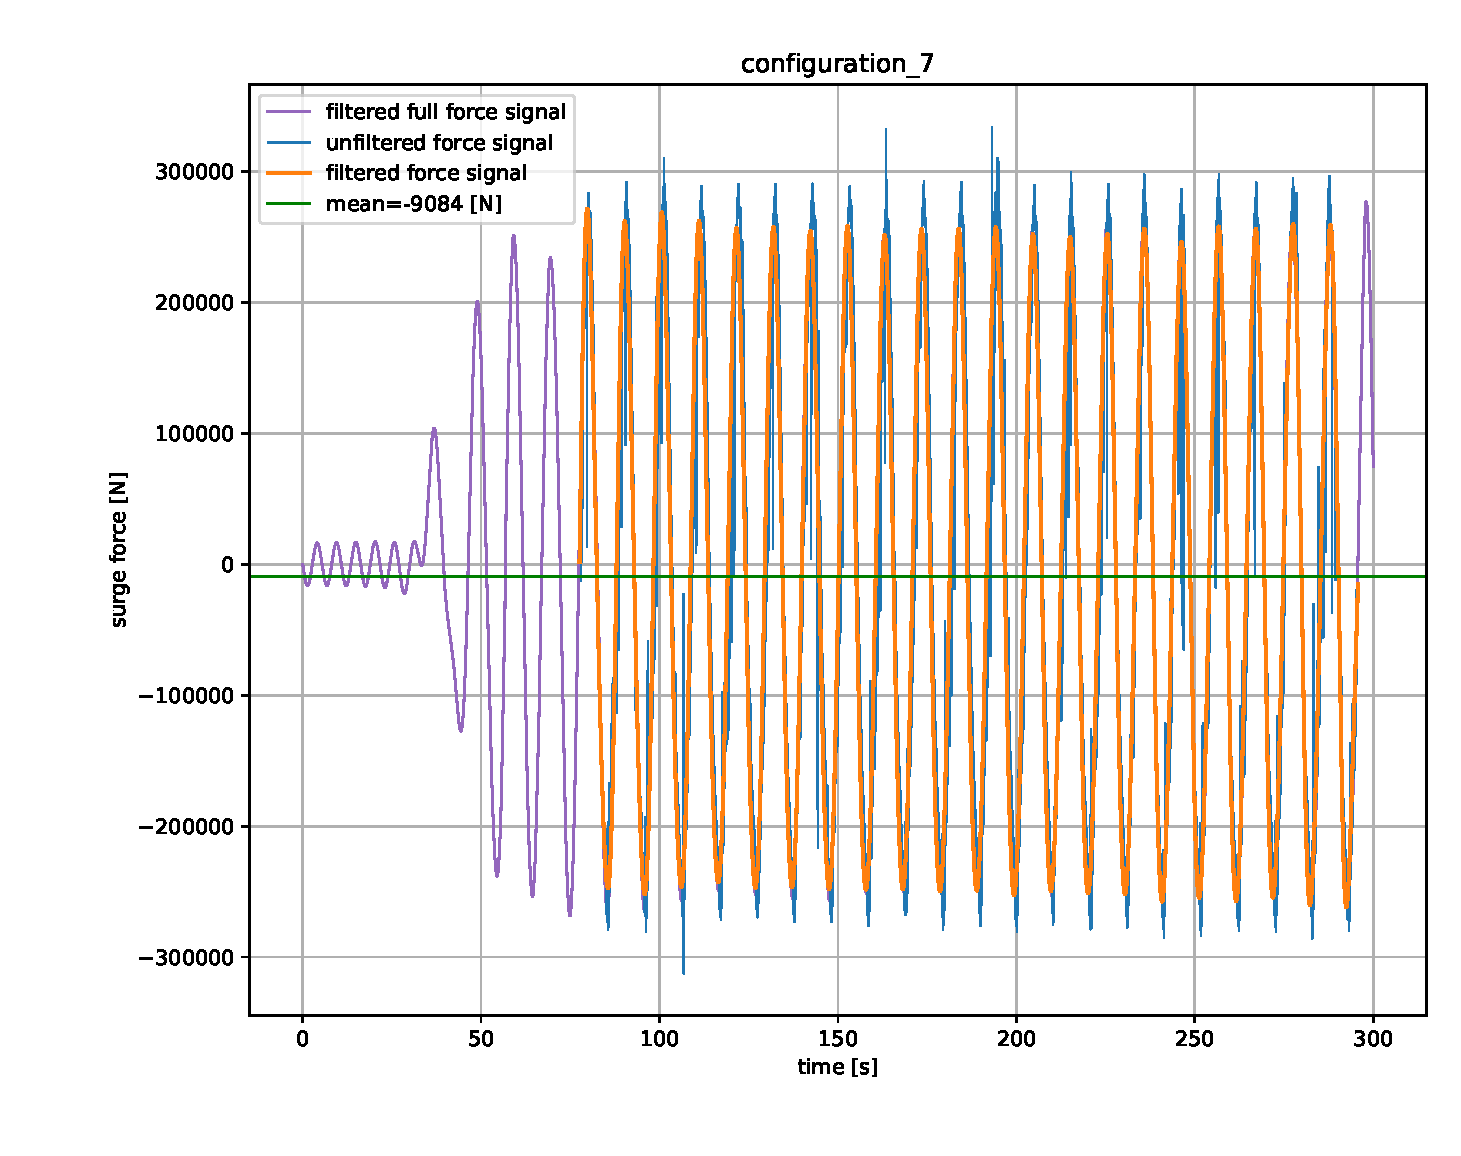
\includegraphics[width=\textwidth]{figures/Methodology/calculation_Fd_mean_methodology.pdf}
        \caption{Force signal used in calculation mean wave drift force}
        \label{fig: methodology Fd calculation}
     \end{subfigure}
     \hfill
     \begin{subfigure}[b]{0.49\textwidth}
         \centering
        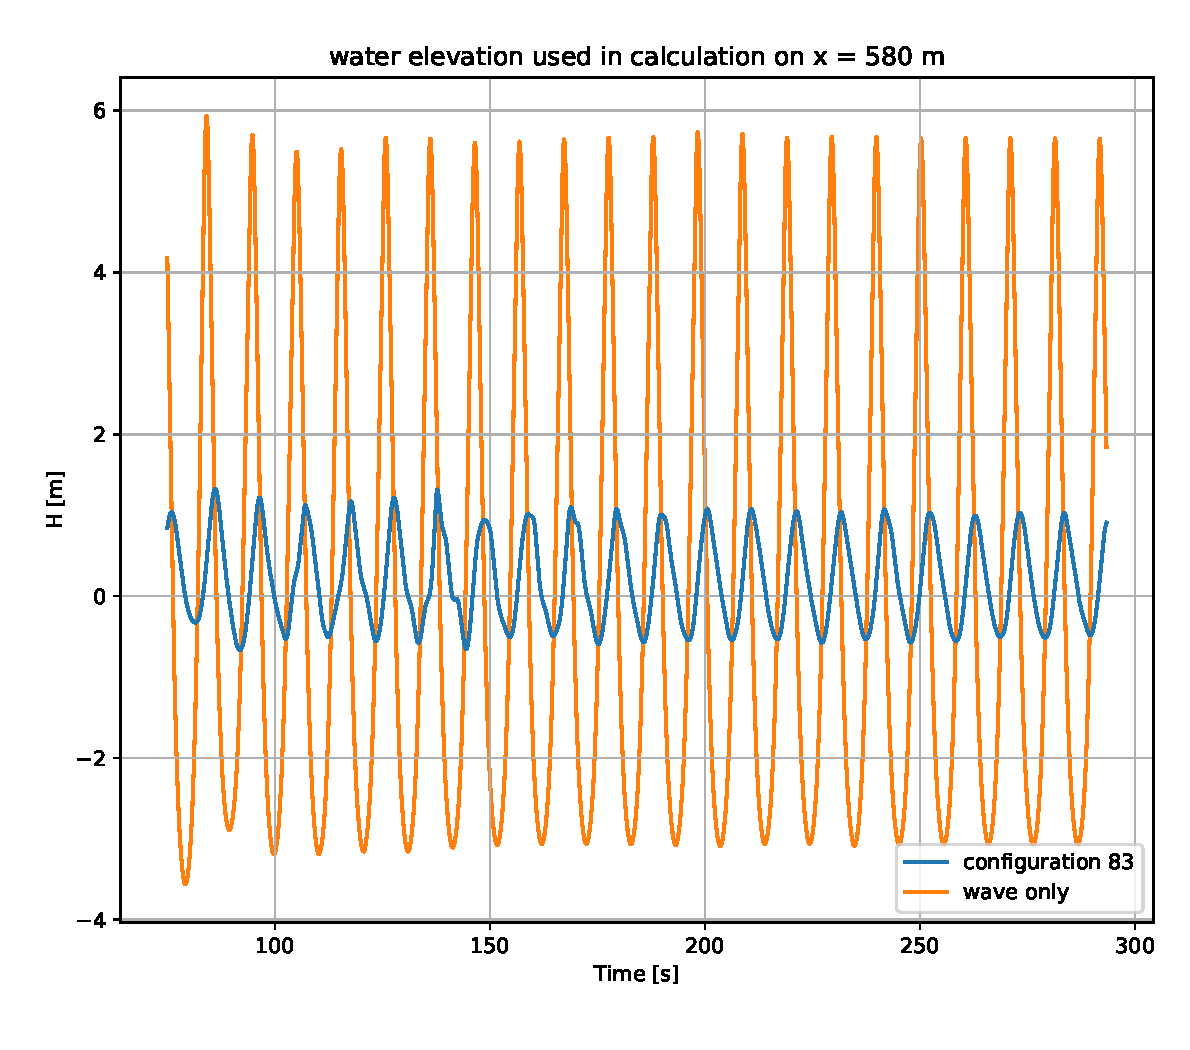
\includegraphics[width = \linewidth]{figures/Methodology/calculation_H_t_methodology.pdf}
        \caption{Wave elevation over time use in calculation wave transmission}
        \label{fig: methodology Kt calculation}
     \end{subfigure}
     \caption{Signals used in post-processing}
\end{figure}

\subsubsection{Wave transmission}
To understand how wave transmission is determined from ComFLOW output, it is necessary to understand how the grid is built, which will be used in the simulations (see Figure \ref{fig: grid used methodology}). The outline of this grid is determined in the validation phase of this thesis, which is extensively discussed in Section \ref{sec: general outline grid}. Here, the waterline is at z = 0, and the waves will be generated at the left boundary (x = 0) and propagate to the right. They will interact with the breakwater, which is placed up to x = 405 m. Therefore, the x-location of the left side (wave-ward) side of the structure depends on its width and its right side (lee-ward) is always placed at x=405m. Figure \ref{fig: zoomed grid used methodology} shows the grid more closely zoomed in on the position where the breakwater is placed. \\
\\
The transmitted wave height $H_t$ will be determined between x = 450 m and x = 580 m. At every cell at the waterline, the wave height over time is logged and can be read in Python. An example of the elevation of the water over time for a single cell (located at x=580m in the domain) of an arbitrarily chosen simulation (excluding run-up) is shown in Figure \ref{fig: methodology Kt calculation}. The average transmitted wave height is determined for every cell between x=450m and x=580m. Averaging this number leads to the value of the transmitted wave height $H_t$. Also, a 'wave-only' simulation is done, where the exact same settings are used, but without any geometry. The average wave height over time between x = 450 m and x = 580 m of this wave-only simulation is what is used as the incident wave height $H_i$ in the calculation of each of the transmission coefficients of the breakwater $K_t~=(H_t/H_i)$. This is done to account for the numerical dissipation that occurs between x = 0m and x = 580m. For this, the function \textit{transmitted\_wave\_height} in the Python script shown in Section \ref{script: post processing functions} of Appendix \ref{app: scripts for post-processing} is used. \\
\\

\begin{figure}[h]
    \centering
    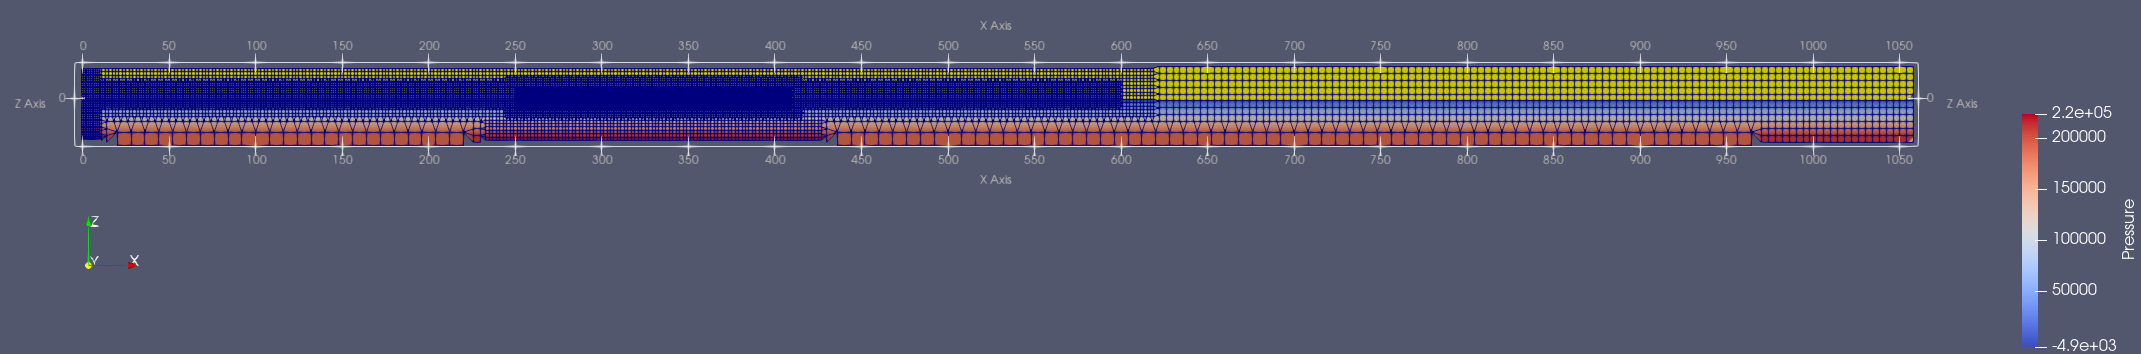
\includegraphics[width=\linewidth]{figures/Methodology/grid2.png}
    \caption{Grid used in simulations}
    \label{fig: grid used methodology}
\end{figure}

\begin{figure}[h]
    \centering
    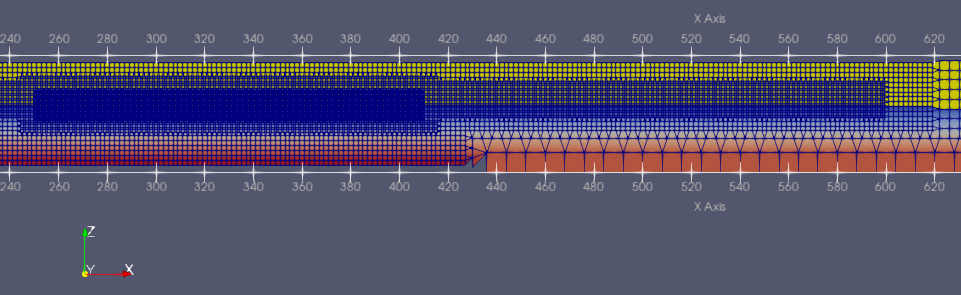
\includegraphics[width=\linewidth]{figures/Methodology/grid zoomed 2.png}
    \caption{Grid used in simulations zoomed}
    \label{fig: zoomed grid used methodology}
\end{figure}



% \section{Test of scripts}

% Breakwaters with simple geometries are used to test whether the scripting of the \acrfull{cob}, mass and radius of inertia is calculated right. These quantities can be easily determined manually for these geometries and compared to the results of the Python script. Once all these quantities match between the hand calculations and the Python scripts, it can be concluded that these quantities are calculated correctly for more complex geometries as well. The geometries from Figure \ref{tab:check breakwaters}, with its parameters given in Table \ref{tab:check breakwaters}, are used for this check.


% % Please add the following required packages to your document preamble:
% % \usepackage{booktabs}
% \begin{table}[h]
% \centering
% \begin{tabular}{@{}lllllll@{}}
% \toprule
% configuration & T [m]  & W [m]   & front\_fraction [-] & top\_fraction [-] & radius [m] & WL [m] \\ \midrule
% 1   & 10 & 100 & 0.00001            & 0.00001          & 2e7 & 2  \\
% 2   & 10 & 100 & 0.00001            & 0.00001          & 2e7 & -5 \\
% 3   & 10 & 100 & 0.99999            & 0.99999          & 2e7 & 2  \\
% 4   & 10 & 100 & 0.99999            & 0.99999          & 2e7 & -5 \\ 
% 5   & 10 & 100 & 0.50            & 0.50          & 2e7 & -8 \\ \bottomrule
% \end{tabular}
% \caption{Parameters of breakwaters}
% \label{tab:check breakwaters}
% \end{table}





% \begin{figure*}[h]
%     \centering
%     \begin{subfigure}[b]{0.475\textwidth}
%         \centering
%         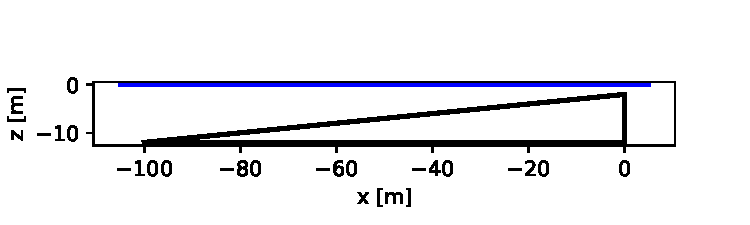
\includegraphics[width=\textwidth]{figures/ComFLOW/Breakwater Geometries/script checks/breakwater_geometry1.pdf}
%         \caption[]%
%         {{\small Configuration 1}}    
%         \label{fig: check Configuration 1}
%     \end{subfigure}
%     \hfill
%     \begin{subfigure}[b]{0.475\textwidth}  
%         \centering 
%         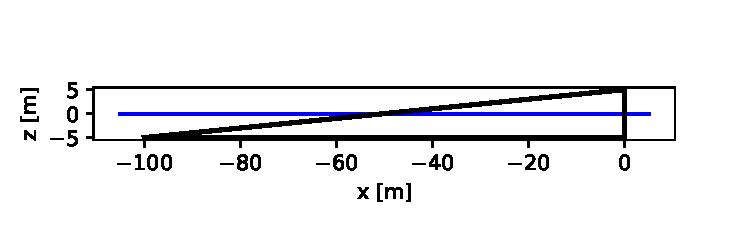
\includegraphics[width=\textwidth]{figures/ComFLOW/Breakwater Geometries/script checks/breakwater_geometry2.pdf}
%         \caption[]%
%         {{\small Configuration 2}}    
%         \label{fig: check Configuration 2}
%     \end{subfigure}
%     \vskip\baselineskip
%     \begin{subfigure}[b]{0.475\textwidth}   
%         \centering 
%         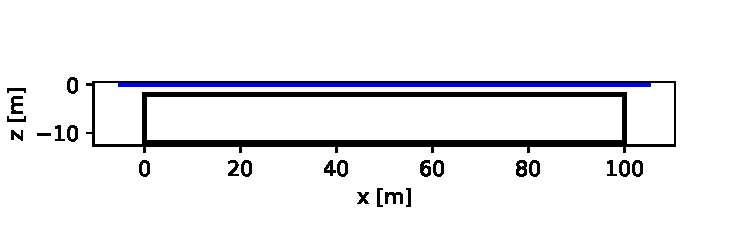
\includegraphics[width=\textwidth]{figures/ComFLOW/Breakwater Geometries/script checks/breakwater_geometry3.pdf}
%         \caption[]%
%         {{\small Configuration 3}}    
%         \label{fig: check Configuration 3}
%     \end{subfigure}
%     \hfill
%     \begin{subfigure}[b]{0.475\textwidth}   
%         \centering 
%         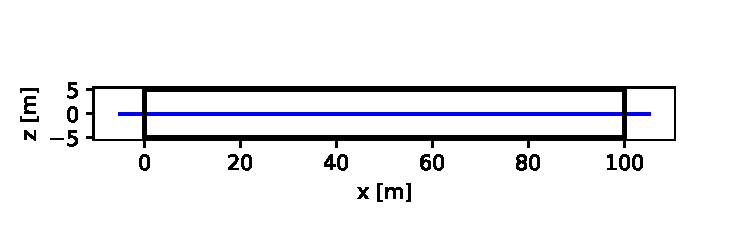
\includegraphics[width=\textwidth]{figures/ComFLOW/Breakwater Geometries/script checks/breakwater_geometry4.pdf}
%         \caption[]%
%         {{\small Configuration 4}}    
%         \label{fig: check Configuration 4}
%     \end{subfigure}
%     \hfill
%     \begin{subfigure}[b]{0.475\textwidth}   
%         \centering 
%         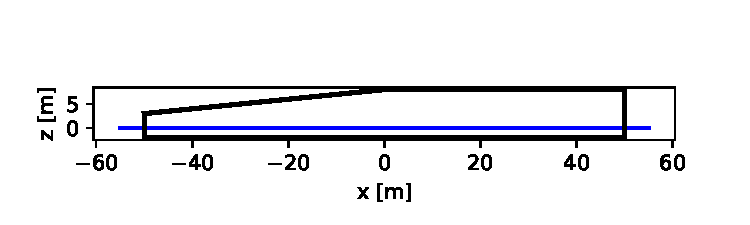
\includegraphics[width=\textwidth]{figures/ComFLOW/Breakwater Geometries/script checks/breakwater_geometry5.pdf}
%         \caption[]%
%         {{\small Configuration 5}}    
%         \label{fig: check Configuration 5}
%     \end{subfigure}
%     \caption{Breakwaters}
%     \label{fig: check Configurations}
% \end{figure*}


% The Python scripts which calculated the mass of the breakwater and the location of the acrfull{cog} for each configuration performed well according to this test. This can be seen in Table \ref{tab:check values hand cal vs P}, where all numbers complied. Except for the location of the acrshort{cog} for configurations where the beach of the breakwater is either partly or fully under water. There they were 1 to 4 cm off, which is negligible on such scales and due to numerical errors in the calculations. 


% \begin{table}[h]
% \begin{tabular}{lllllll}
% \hline
%               & \multicolumn{3}{l}{Hand calculations}                   & \multicolumn{3}{l}{Values Python scripts}               \\ \hline
% configuration & mass {[}kg{]} & x$_{CoG}$ {[} m{]} & z$_{CoG}$ {[} m{]} & mass {[}kg{]} & x$_{CoG}$ {[} m{]} & z$_{CoG}$ {[} m{]} \\ \hline
% 1 & 5.00e5 & -33.33 & -6.67 & 5.00e5 & -33.37 & -6.67 \\
% 2 & 3.75e5 & -38.89 & -7.77 & 3.75e5 & -38.86 & -7.78 \\
% 3 & 1.00e6 & 50.00  & -5.00 & 1.00e6 & 50.00  & -5.00 \\
% 4 & 5.00e5 & 50.00  & -7.50 & 5.00e5 & 50.00  & -7.50 \\
% 5 & 2.00e5 & 50.00  & -9.00 & 2.00e5 & 50.00  & -9.00 \\ \hline
% \end{tabular}
% \caption{Values of hand calculations versus values out of Python scripts}
% \label{tab:check values hand cal vs P}
% \end{table}


% Also, with these and more floaters still water tests are performed, where the breakwater were tested for 300 seconds in the water without the interference with waves to see whether the mass and acrshort{cog}  are scripted correctly. No strange behaviour was observed, the breakwaters did not move.



\section{Cost Function}
\label{sec: cost analysis methodology }
In this section the cost function is introduced which determines the total cost reduction on the system due to the presence of the breakwater. This cost function consists of three parts. In the first part, the mooring system of the floating island of the North Sea case of Space@Sea is decomposed in \ref{sec: mooring costs}. This is used to determine the cost reduction provided by the breakwater, which is discussed in Section \ref{eq: reduction mooring costs}. Finally, the construction costs of the breakwater are estimated using a cost function presented in Section \ref{sec: breakwater costs}.



%Also, the floating island will experience less motions when the right breakwater is placed, which increases the workability on the island modules and connector costs will be less. Therefore, a cost function which quantifies these effects as function of the breakwaters transmitted wave height will be introduced in Section \ref{sec: work and connector costs}.


\subsection{Mooring costs}
\label{sec: mooring costs}

% An estimation was made for the mooring costs by using the the public deliverable D1.3 from Space@Sea. In this document is referred to a document where the exact composition of the mooring costs can be found. Unfortunately, this document is confidential. Thereby, an estimation was made by the following calculation. D1.3 gave a total of \texteuro 20 M for the total mooring system of the floating island, schematized by the following picture

% -estimation mooring costs Space@Sea\\
% -Delivarable 1.3: total mooring system costs \texteuro 20 M\\
% -So, one row of breakwaters would cost roughly \texteuro 20/9 M.
% -That mean wave drift force scales linearly with the amount of euros 


In Space@Sea, extensive research is done by \citet{D3.3space@sea} on the design of the mooring system of the North Sea case, based on the wind, wave and current conditions at that location (see Section \ref{sec:intro background} for the exact location). This design of the mooring system, with its costs, is taken as a benchmark for estimating the reduction in mooring costs. First, we investigate how the mooring design was constructed in order to make an as accurate as possible cost function for the future mooring costs of what the mooring system would cost when a breakwater is present. The total costs of the mooring system was estimated by \citet{D3.3space@sea} at \texteuro 20 M. Since a 2D breakwater is studied in this thesis, everything is calculated per unit width. Therefore, this set-up is simplified to a single row of nine island modules. It is assumed that this will cost $\frac{1}{9}$ of the total mooring costs, which is approximately \texteuro 2.22 M. Dividing this by 45 (= module width) leads to \texteuro 49.382,71 per unit width of the floating island.  This design is made based on a peak mean wave drift force of 120.7 MN, which is caused by the wind, current, and waves. In the following sections, the magnitude of the contribution of each phenomenon is investigated. 


\begin{figure}[h]
    \centering
    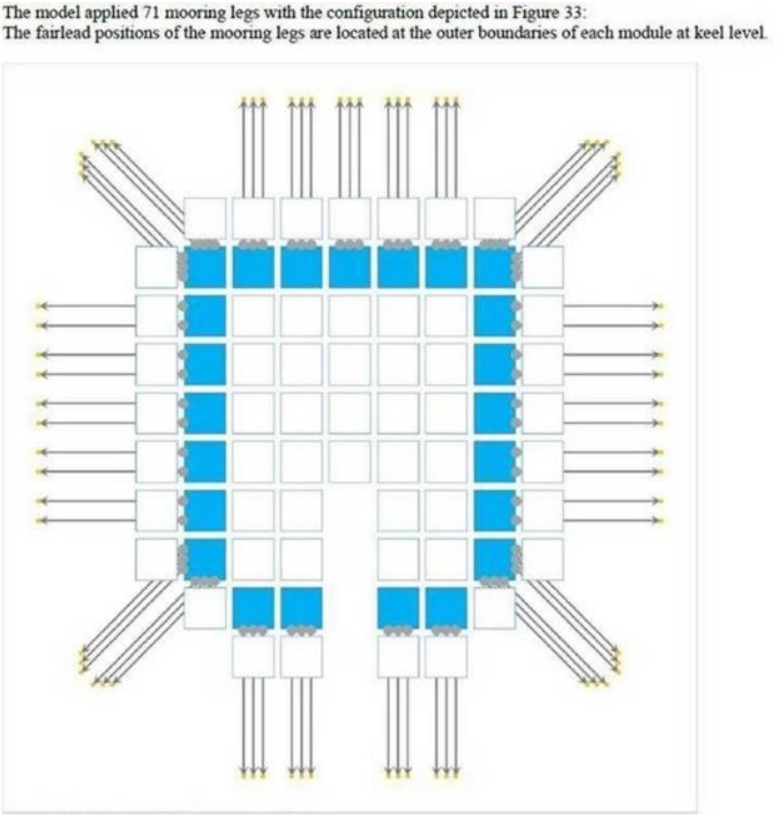
\includegraphics[width=0.5\linewidth]{figures/Costs/mooring_layout.PNG}
    \caption{Mooring layout Space@Sea. Source: \citep{S@S1.3}}
    \label{fig: mooring layout S@S}
\end{figure}



\paragraph{Wind Load}
The contributions of the wind loads are applied using the following \acrfull{OCIMF} convention \cite{D3.3space@sea}:
\begin{equation}
    F_{x,w} = \frac{1}{2} \cdot \rho_a \cdot C_{x,w} \cdot V_w^2 \cdot A_T
\end{equation}
In the design of the Space@Sea mooring system, the following parameters are used:
\begin{itemize}
    \item Air density $\rho_a$ = 1.225 $kg/m^3$
    \item Coefficient $C_{x,w}$ = 1
    \item Wind velocity $V_w$ = 29.5 $m/s$
    \item Transverse surface area above water $A_T$ = 225 $m^2$
\end{itemize}
This results in a design wind load per unit width of $F_{x,w}~\approx$ 239.86 kN. Dividing this through the width of the floater gives a wind design load of $F_{x,w}~\approx$ 5.33 kN/m

\paragraph{Current Load}
The current load used for the design of the Space@Sea mooring system is calculated according to the \acrshort{OCIMF} convention as well:
\begin{equation}
    F_{x,w} = \frac{1}{2} \cdot \rho_w \cdot C_{x,c} \cdot V_c^2 \cdot W \cdot T
\end{equation}
where the following parameters are used:
\begin{itemize}
    \item Seawater Density $\rho_w$ = 1000 $kg/m^3$
    \item Coefficient $C_{x,c}$ = 1
    \item Current velocity $V_c$ = 2.0 $m/s$
    \item Module width $W$ = 45 $m$
    \item Module depth $T$ = 6 $m$
\end{itemize}
This results in a current design load of $F_{x,c}~ = $ 540.00 kN. Per unit width this is $F_{x,c}~ = $ 12.00 kN/m\\
\\
\paragraph{Wave load}
The maximum mean wave drift force used in the design of the mooring system of the entire island (see Figure \ref{fig: mooring layout S@S}) is 120.7 MN \cite{D3.3space@sea}. Per unit width, this is 297.93 kN/m. From which 12.00 kN/m is due to the current and 5.33 kN/m is due to the wind. So, the contribution to the mean wave drift force delivered by the waves is 280.60 kN/m, which is 94 \% of the total mean wave drift force.\\
\\
This big proportion of the contribution of the waves to the maximum mean wave drift on the island emphasises the potential added value the breakwater can have, but does not mean that we can neglect the other contributions by the wind and the current. Six per cent may seem negligible, but when a breakwater succeeds in attenuating the waves substantially, these ratios will be very different. Especially since the height of the mean wave drift force on the floating island scales to the height of the waves interacting with the island squared. Therefore, the breakwater can only contribute in lowering 94\% of this force, the 6\% due to the wind and current will always stay included. This is more elaborated in the folowing section. 


\subsection{Reduction of mooring costs due to the presence of breakwater}
\label{subsec: reduction mooring costs function}
This section explains how the results of the last section are used for the cost function of the cost reduction in mooring costs, due to the presence of the breakwater. First, the cost function is symbolically shown in equations \ref{eq: new mooring island costs} to \ref{eq: reduction mooring costs}, using the relations shown in \ref{eq: relations cost function}. Then, the same cost function is clarified using text and figures.



% The rest of the section explains how the reduction of mean wave drift forces on the floating island quantifies in a reduction of mooring costs. In \cite{D3.3space@sea} is stated that the mooring system is designed for a peak mean wave drift force of 120.7 MN. To convert this to a single row of modules again, $\frac{1}{9}$th of that force will be 13.4 MN and dividing this through 45 leads to 0.30 MN of design drift force per unit with of floating island. The mean wave drift force scales to the height of the incoming wave squared. Together with the assumption that the cost of the mooring system scales linearly to the mean wave drift force acting on the island, the reduction on mooring costs is derived as follows.


\begin{equation}
\begin{array}{lll}
    H^2 & \propto \bar{F_d}\\
    \\
    \bar{F_d} & \propto \texteuro_{mooring} \\
    \\
    \texteuro_{mooring} & \propto H^2
\end{array}
\label{eq: relations cost function}
\end{equation}


% \begin{equation}
% \begin{array}{lll}
%     \text{\texteuro}_{new~mooring~island} = \text{\texteuro}_{old~mooring~island} \cdot \frac{H_{t,breakwater}}{H_{i,breakwater}}^2\\
%     \\
%     \text{\texteuro}_{mooring~breakwater} = \text{\texteuro}_{old~mooring~island} \cdot \frac{\bar{F_{d, breakwater}}}{F_{peak S@S island}}\\
%     \\
%     \text{\texteuro}_{new~total~mooring} = \text{\texteuro}_{new~mooring~island} + \text{\texteuro}_{mooring~breakwater}

% \end{array}
% \end{equation}

Leads to
\begin{equation}
    \text{\texteuro}_{new~mooring~island} =  \text{\texteuro}_{old~mooring~island} \cdot (0.06+ 0.94\cdot \frac{H_{t,breakwater}}{H_{i,breakwater}}^2)
    \label{eq: new mooring island costs}
\end{equation}
\begin{equation}
    \text{\texteuro}_{mooring~breakwater} = \text{\texteuro}_{old~mooring~island} \cdot \frac{\bar{F}_{d, breakwater}}{\bar{F_{d, old~island}}}\\
    \label{eq: mooring costs breakwater}
\end{equation}
\begin{equation}
    \text{\texteuro}_{new~total~mooring} = \text{\texteuro}_{new~mooring~island} + \text{\texteuro}_{mooring~breakwater}
    \label{eq: total mooring costs}
\end{equation}
\begin{equation}
    \texteuro_{reduction~mooring~costs}  = \texteuro_{old~mooring~island}- \texteuro_{new~total~mooring}
    \label{eq: reduction mooring costs}
\end{equation}





\begin{figure}[h]
 
    \centering
    \begin{subfigure}[b]{0.99\textwidth}
        \centering
        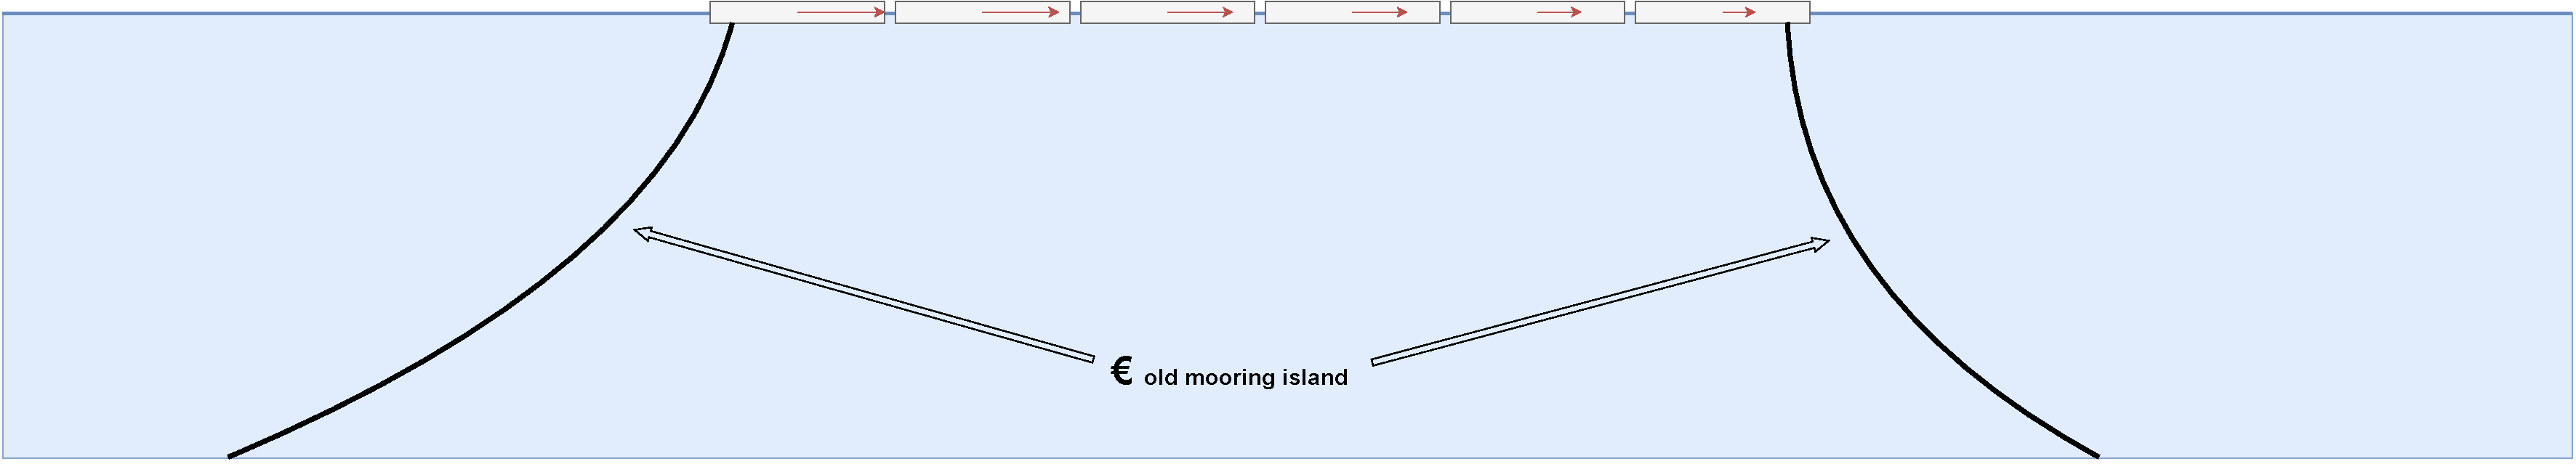
\includegraphics[width=\linewidth]{figures/Methodology/floatingisland_oldmooring.pdf} 
        \caption[]%
        {{\small Floating island without breakwater}}    
        \label{fig: old floating island cost function}
    \end{subfigure}

    \centering
    \begin{subfigure}[b]{0.99\textwidth}  
        \centering 
        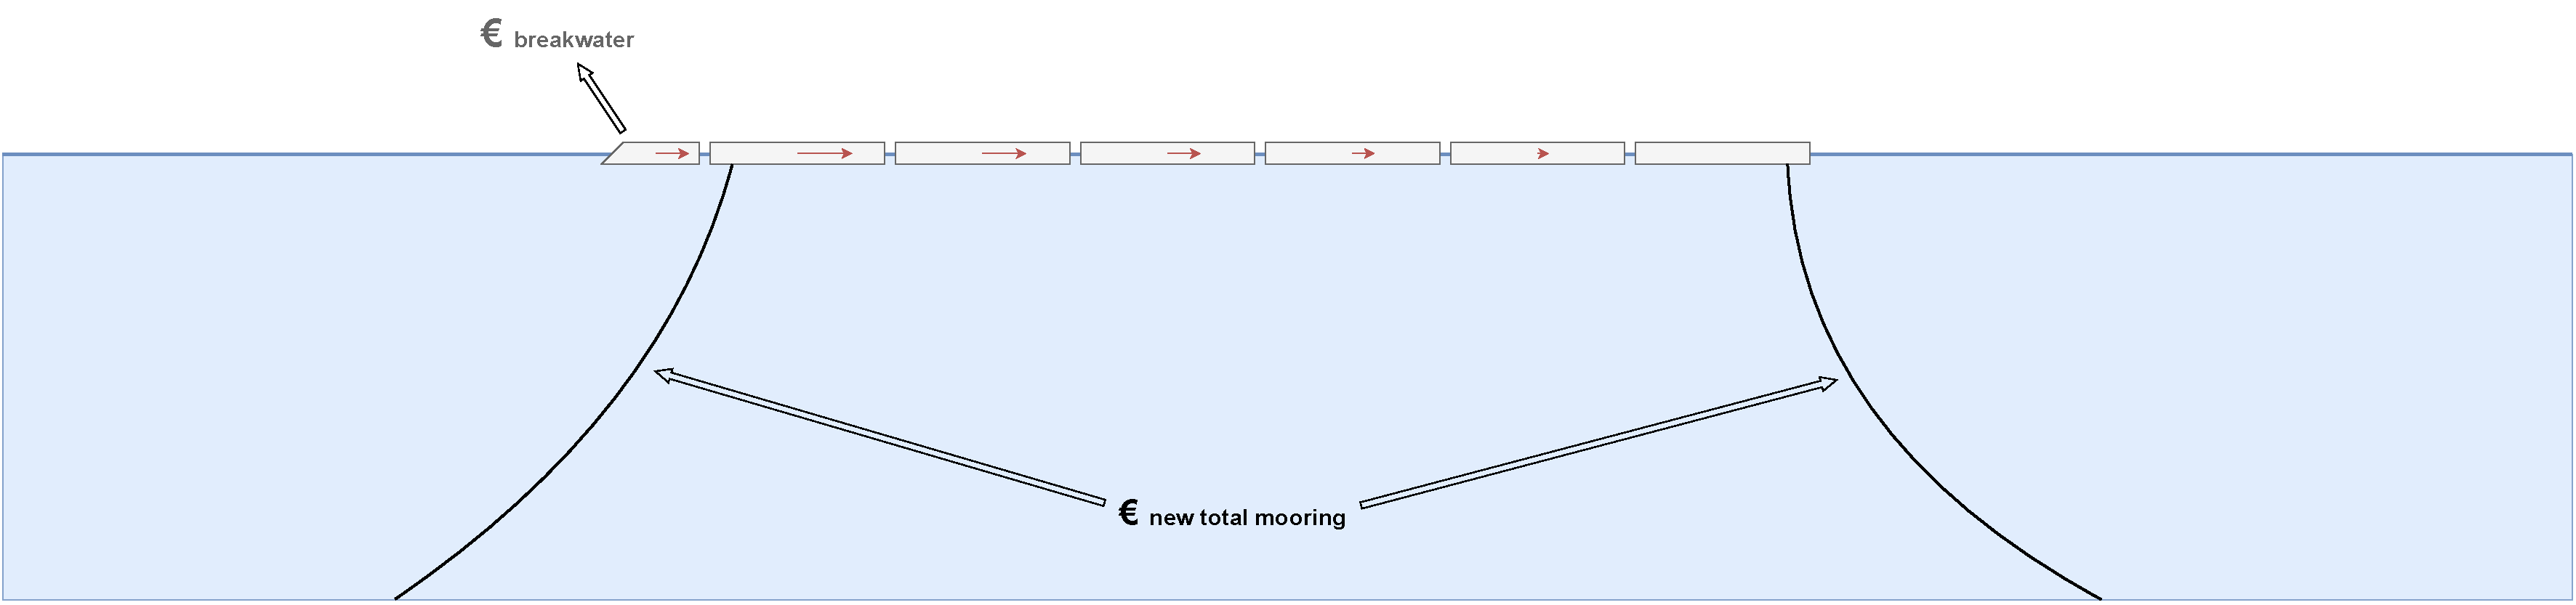
\includegraphics[width=\linewidth]{figures/Methodology/floatingisland_newmooring.pdf}
        \caption[]%
        {{\small Floating island with breakwater}}    
        \label{fig: new floating island cost function}
    \end{subfigure}



    \caption{}
    \label{fig: }
\end{figure}





The "old" floating island is the Space@Sea North Sea case, without breakwater, is schematically shown in Figure \ref{fig: old floating island cost function}. The mean wave drift force must be countered with a mooring system. The costs of this mooring system of the "old" floating island are denoted by \texteuro$_{old~mooring~island}$ and have a value of 49.382,71 \texteuro/m. 


The "new" floating island is the same system, but with a breakwater connected to its wave-ward side. This system is schematically shown in Figure \ref{fig: new floating island cost function}. The total mooring costs of this "new" floating island are denoted by \texteuro$_{new~total~mooring}$, which is constructed by the mooring costs of the breakwater and the new mooring costs of the island. The new mooring costs for the island are denoted by \texteuro$_{new~mooring~island}$ and will be lower than \texteuro$_{old~mooring~island}$, because the breakwater attenuates the wave energy. The transmitted wave height (wave height behind the breakwater) still causes the floating island at its lee-side to have a mean wave drift force. Therefore, the ratio between the transmitted wave height and the incident wave height is used in the calculation of \texteuro$_{new~mooring~island}$ in Equation \ref{eq: new mooring island costs}.  As can be seen in this equation, the transmission coefficient ($H_t/H_i$) has only an influence on 94\% of the new mooring costs. In other words, when 100\% of the wave is attenuated by the breakwater ($H_t/H_i$ = 0), there are no drift forces due to the waves, but the current and wind can still put a load on the mooring lines and 6\% of the old mooring costs will still be present.\\
The breakwater itself also experiences a mean drift force of the waves, which contributes to the total costs of the mooring system. This contribution is denoted by \texteuro$_{mooring~breakwater}$ and is calculated by the ratio of its mean wave drift force $\bar{F}_{d, breakwater}$ and the maximum mean wave drift force used in the design of the "old" mooring system: F$_{d, old~island}$, which is 0.30 MN/m (120.7 MN computed to per unit width). \\
Finally, the total reduction in mooring costs due to the presence of the breakwater, denoted with \texteuro$_{reduction~mooring~costs} $ is the difference between the costs of the "old" mooring system and the "new" system (equation \ref{eq: reduction mooring costs}).



% which is computed via the ratio between the transmitted wave height and the incident wave height



% The breakwater attenuates the wave energy and thereby reduces the mean wave drift force experienced by the island. 


% All quantities are per unit width. In the formula \ref{eq: new mooring island costs}, the design mooring costs of \texteuro 49.382,71 is used for $\text{\texteuro}_{old~mooring~island}$, and the ratio between the transmitted wave height and the incident wave height is used with the calculation of $\text{\texteuro}_{new~mooring~island}$, which is the new height off the mooring costs of the floating island due to the wave attenuation of the breakwater. The transmission coefficient ($H_t/H_i$) has only an influence on 94\% of the new mooring costs. In other words, when 100\% of the wave is attenuated by the breakwater ($H_t/H_i$ = 0), no drift forces are present due to the waves, but the current and wind can still give a load on the mooring lines and 6\% of the old mooring costs will still be present.\\
% Formula \ref{eq: mooring costs breakwater} defines the costs of the mooring system of the breakwater itself, using again the design costs of the floating island of Space@Sea times the ratio of the mean wave drift force on the breakwater and the mean wave drift force where the design mean wave drift force of the Space@Sea island. Note that this quantity can be negative when a negative mean wave drift force on the breakwater is experienced.\\



% The outcome of the two latter formulas leads to the total costs of the mooring system: $\text{\texteuro}_{new~total~mooring}$ in formula \ref{eq: total mooring costs} and this is used to calculate the eventual reduction in mooring costs due to the presence of the breakwater $\texteuro_{reduction~mooring~costs}$ in \ref{eq: reduction mooring costs}.








\subsection{Breakwater costs}
\label{sec: breakwater costs}


For the costs of the breakwater, it is assumed that the construction is made of steel and concrete. This material is relatively inexpensive and makes a good combination because concrete is resistant to compression and steel to tension, while they have roughly the same thermal expansion coefficient. In Deliverable 1.2 of the Space@Sea project (\cite{Adam2017D1.2S@S}), a business case is made for an energy hub that aims to provide accommodation and work space for offshore workers. Comprehensive research is done on what the costs would be of such floating structures. Here, it is estimated that the steel and concrete carcass of the structure would have a mass of 9300 ton and would cost \texteuro 9.611.077. From this 9300 ton, 5407 ton (58\%) would be steel and 3893 ton (42\%) concrete. The price of concrete is roughly 775 \texteuro/ton and the price of steel varies from 2000 \texteuro/ton to 4000 \texteuro/ton, depending on the labour needed to manufacture the construction. These prices and mass ratios are used to estimate the \acrshort{capex} costs of the breakwater. So the height of the steel price is different for each breakwater. A box-type structure can be made for 2000 \texteuro/ton and a skew floating beach can be made for 4000 \texteuro/ton. This variation is made into a function the following way; the rectangular parts of the breakwater are made for 2000 \texteuro/ton and the variable part varies between 2000 and 4000 \texteuro/ton (red part in Figure \ref{fig: steel price breakwater}), depending on the angle $\alpha$ with the following formula:
\begin{equation}
    for ~ 0\textdegree ~\alpha<45 \textdegree~:~ \texteuro_{steel} = 4 - \frac{2}{45} \cdot alpha
\end{equation}
\begin{equation}
        for ~ 45\textdegree~<\alpha<90\textdegree ~:~\texteuro_{steel} =\frac{2}{45} \cdot alpha
\end{equation}
\begin{figure}
    \centering
    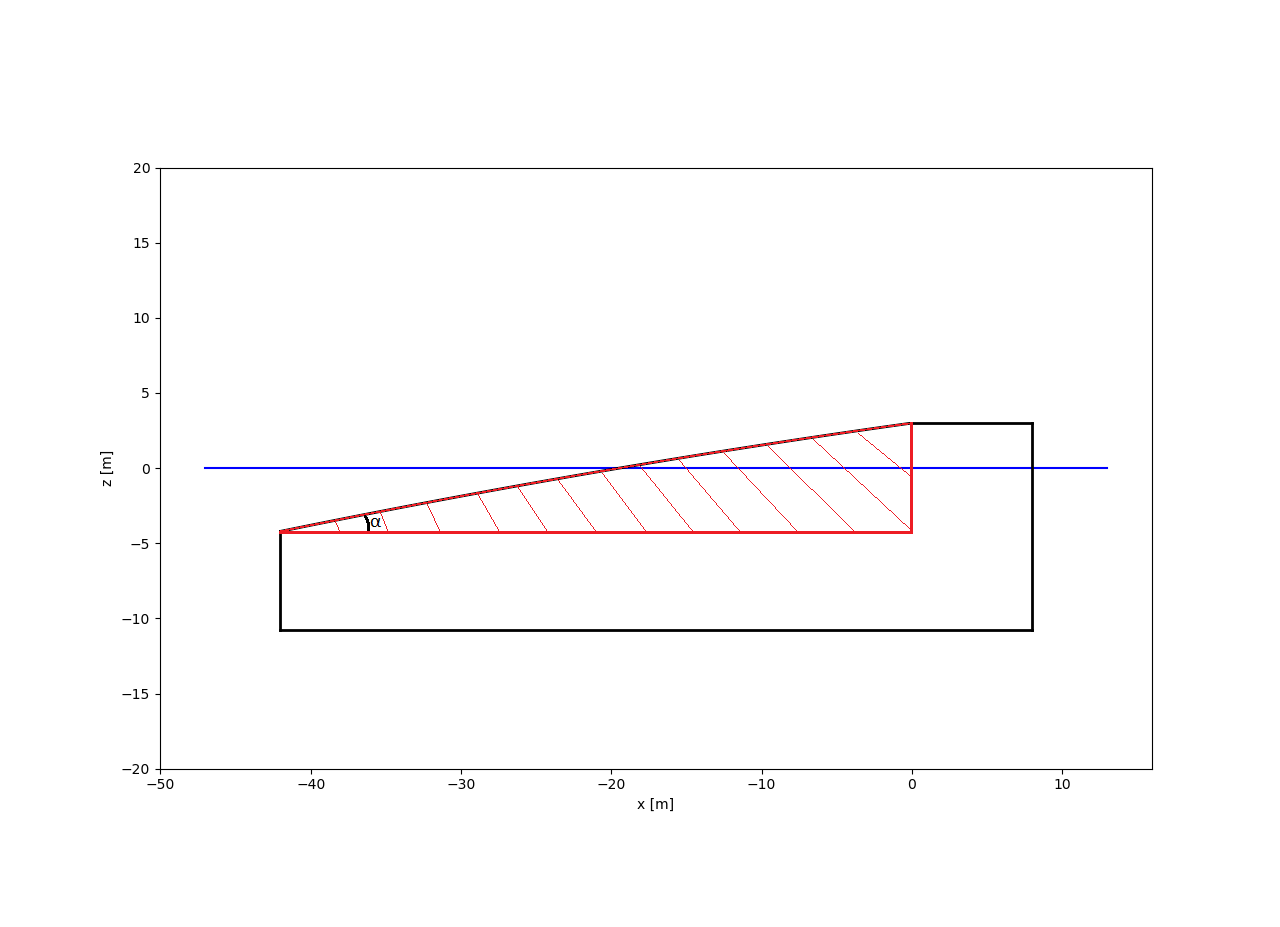
\includegraphics[width=0.5\linewidth]{figures/Costs/breakwater_1.png}
    \caption{Part where steel price is variable}
    \label{fig: steel price breakwater}
\end{figure}
In this way, the price reaches its maximum (4000 \texteuro/ton) when a very skew slope is desired and its minimum (2000 \texteuro/ton) when $\alpha=45 \textdegree$. \\
\\
Now the prices for all parts of the breakwater are known. The only thing missing is the total price of the structure. Therefore, the energy hub of the Space@Sea project is again taken as a benchmark. The steel and concrete carcass of this hub will be approximately \texteuro 9.611.077 and have dimensions of: WxBxH = 45m x 45m x 10 m. Per unit width, the price is approximately 213.580 \texteuro/m. Dividing this by the circumference in the xz-plane (45$\cdot$10=450 m$^2$) results in approximately 475 \texteuro/m$^3$, which is the price of the steel and concrete carcass of the energy hub per unit width per unit circumference. Multiplying this number by the circumference of the breakwater almost gives the construction price of the breakwater. The only thing left to do is multiply the result by a fraction so that the steel used on the beach slope is made for the variable steel price and the steel used on the rest of the breakwater for \texteuro 2000 euro/ton. The way this price is calculated in Python is shown in the function '\textit{geometry\_costs\_function2}' in Appendix \ref{app: scripts for post-processing}.\\
\\
Of course, the market price of concrete can also vary in time, but the amount of labour put into the manufacturing of the concrete is hardly affected by the shape of the breakwaters. It is poured in fluidly after the framework is created and takes on the proper shape by itself. Thus, the price of concrete is assumed to be constant with a price of 775 \texteuro/ton for the breakwaters. \\



\chapter{Validation and grid design ComFLOW}
\label{ch: validation comflow}
In this thesis, a breakwater is designed to provide shelter to a floating island from incoming waves. To arrive at the best design, the hydrodynamic behaviour of different geometries must be analysed, to assess which design offers the best performance. To simulate multiple variations of the geometry, a \acrshort{cfd} software method is used: ComFLOW. This method numerically solves the Navier-Stokes equations, and thereto, the computational domain is covered by a fixed Cartesian grid. A coarser grid generally means faster simulations, so a coarse grid is desired to save computational power and maximise the total number of simulations performed in a limited amount of time.  On the other hand, the grid must be fine enough to give reliable results that converge to a static value. In other words,  the result of the final grid must be the same as when the grid is refined further. And the comparison must be made with reality, to quantify the deviation from the ComFLOW result, to be able to draw conclusions from the simulations.\\
\\

Also, ComFLOW comes with a lot of different settings. The effects of different settings and different grids were extensively analysed during the first months of this graduation thesis. This resulted in certain settings and grid characteristics that gave the best performance, which are presented in the following sections. So, only the most important and useful results of this extensive analysis are discussed. The ComFLOW settings used are introduced in Section \ref{sec: possible settings ComFLOW}, and the outline of the grid is explained in \ref{sec: general outline grid}. Different refinements of this outline are analysed in sections \ref{sec: prop of free surface waves} and \ref{sec: box-type breakwater}. Where \ref{sec: prop of free surface waves} studies the propagation of free surface waves through the domain without interference with a geometry, to quantify the numerical dissipation and reflection at the boundaries and refinement edges. And \ref{sec: box-type breakwater} compares the results of ComFLOW when regular waves interfere with a box-type breakwater with linear wave theory. Finally, the dissipation of wave energy through wave breaking in ComFLOW is tested by comparing its results with an experiment in which waves plunged over a breaker bar in Section \ref{sec: Dissipation}, performed by \citet{breakerbarexperiment}.


% -grid generation: realistic results, but most efficient in terms of computation time/expensiveness\\
% -checked by three different methods, first the settings are chosen in which less numerical dissipation as possible is achieved, to check the average wave height over the complete length of the domain. (in first paragraph)\\
% -reflection is validated by the Macagno formula and the forces experienced (second paragraph).\\
% -An experiment with a breaker bar is mimicked to validate the model on dissipation


\section{Settings ComFLOW}
\label{sec: possible settings ComFLOW}
ComFLOW can be used with lots of different settings, integration and convection schemes, wave models, etc. Various wave settings that are applicable to this thesis are studied and discussed in this section. Most of the information comes from the ComFLOW reference page \parencite{poseidon_comflow_reference_page}. Also, the final settings used that gave the best performance are given in this section.

\subsection{Integration method}

Two different integration methods can be used: Forward-Euler and Adams-Bashforth. Forward Euler is a single-step method which refers to only one previous point and its derivative to determine the current value. Adams-Bashforth is a two-step explicit method. The influence of both methods on the simulation results and computation time was found to be negligible.\\
\\
\textbf{Adams-Bashfort was chosen for future simulations.}

\subsection{Boundary conditions}
At the boundaries of the domain, the inflow and outflow conditions can be specified. The various types are
\begin{itemize}
    \item Basic inflow condition: Imposes incoming flow by means of a Dirichlet condition for the velocity and the water level. 
    \item \acrfull{gabc}: An extension of the Sommerfield boundary condition (using a wave velocity, which is calculated from the wave period and wave number) with an approximation of the linear dispersion relation in terms of $k h$, in combination with vertical derivatives of the solution variables \parencite{Wellens2020}. 
    \item Pressure Neumann: The Neumann boundary condition is obtained by applying the normal component of the momentum equation at the boundary \parencite{Abdallah1988} 
    
    % Pressure and water height in the exterior of the domain are approximated using constant extrapolation. This is a very simple boundary condition and does not perform very well in wave simulations.
    \item Pressure Dirichlet: The Dirichlet boundary condition is obtained by integrating the tangential component of the momentum equations along the boundary \parencite{Abdallah1988}.
    \item Free slip: At free-slip boundaries, the tangential velocities in the exterior are set equal to those in the interior such that the viscous stresses become zero. The liquid distribution is assumed to be uniform across the boundary. 
\end{itemize}


\textbf{The \acrshort{gabc} was found to be the best performing in terms of stability and reflection and is used for future simulations.}

\subsection{Numerical settings}
\label{subsec: numercial settings validation}
\subsubsection{Linear solver}

The linear solver is used for solving the pressure Poisson equations, and when quasi-implicit discretization is used for diffusion, the solver is also used for solving the intermediate solution of the momentum equations. The different options are as follows:
\begin{itemize}
    \item \textbf{BiCGSTAB + ILU} preconditioner with special drop tolerance. 
    \item \textbf{SOR} with improved search algorithm. 
\end{itemize}
Only the first of the listed solvers (\textbf{BiCGSTAB + ILU}) is compatible with all ComFLOW simulation settings. The preconditioner in this solver takes care of the special matrix structure near the GABC boundaries and is able to cope with large density variations in two-phase flow simulations.\\
For most one-phase simulations, the solver \textbf{SOR} provides a satisfactory alternative. The \textbf{SOR} solver cannot be used for two-phase simulations or simulations that include a GABC boundary condition.\\
There are more options, but they do not support local grid refinement and have not been parallelised. 

\textbf{The first mentioned: BiCGSTAB + ILU will be used for future simulations}

\subsubsection{Stopping criterion}
The number of solver iterations is determined by two mechanisms. First, the number of iterations is bounded by the setting: 'iter\_max'. This value should be chosen large enough to allow the solver to reach the desired precision and small enough to minimise computational demand.  Second, the solver iterations are controlled by the residual tolerance. In general, smaller values result in more iterations, but improve the accuracy of the solution. The convergence behaviour (error w.r.t. iteration count) depends on the chosen solver. A value of "1.0E-6" is generally a good value, but a useful value in the case of \textbf{wave simulations is "1E-8", so this value will be used for future simulations.}


\subsubsection{Convection scheme}
ComFLOW supports two categories of discretization schemes for convection:
\begin{itemize}
    \item First-order upwind
    \item Second-order central
\end{itemize}
These schemes handle the discretization of convective terms in finite-volume equations. To illustrate both methods, consider the following one-dimensional linear advection term.
\begin{equation}
\frac{\partial u}{\partial t}+a \frac{\partial u}{\partial x}=0
\label{eq: discretization wave}
\end{equation}
It describes a wave propagating in the x-direction with velocity \textit{a}. This can be discretised as
\begin{equation}
\begin{array}{ll}
\frac{u_{i}^{n+1}-u_{i}^{n}}{\Delta t}+a \frac{u_{i}^{n}-u_{i-1}^{n}}{\Delta x}=0 & \text { for } \quad a>0 \\
\\
\frac{u_{i}^{n+1}-u_{i}^{n}}{\Delta t}+a \frac{u_{i+1}^{n}-u_{i}^{n}}{\Delta x}=0 & \text { for } \quad a<0
\end{array}
\end{equation}
where \textit{n} refers to the dimension in time t and \textit{i} refers to the dimension in space x. So, cell \textit{i-1} is the cell left to cell \textit{i} and \textit{i+1} right of \textit{i}. If \textit{a} is positive, the travelling wave solution of the above equation propagates towards the right, the left side of \textit{i} is called the \textit{upwind} side and the right side is the \textit{downwind} side. When \textit{a} is negative, it is the other way around.\\
\\
The second-order central discretization of equation \ref{eq: discretization wave} looks like
\begin{equation}
    \frac{ u_{i}^{n+1}-u_{i}^{n}}{\Delta t}+a \frac{u_{i+1}^{n}- 2u_{i}^{n} + u_{i-1}^{n}}{\Delta x}=0 
\end{equation}
What is good to note, is that the second-order central method uses three cell points in each discretisation, while the first-order upwind method uses two cells. \textbf{The first-order upwind scheme tends to be more stable and gives better dissipation characteristics, so will be for future simulations.} This is elaborated more in \ref{subsec: breakerbar on convection scheme} 


\subsection{Wave model}
An important application of the ComFLOW programme is the simulation of wave impact on offshore structures. ComFLOW provides various built-in wave models, as well as the possibility to import custom data by means of plug-ins. By means of plug-ins and coupling to other software, it is possible to simulate a wide range of other wave conditions (e.g. irregular waves). Wave models can be used for initialisation or as input for boundary conditions.
\subsubsection{Airy wave theory}
The Airy wave model defines the wave elevation by a cosine:
\begin{equation}
    \eta(x,t) = A\cos(\omega t - kx + \epsilon) 
\end{equation}
where $A$ is the amplitude $\omega$ the frequency, $k$ the wave number, and $\epsilon$ the phase.

\subsubsection{Stokes wave theory}
ComFLOW provides second-order and fifth-order Stokes wave models, which are a nonlinear and periodic surface wave.

\subsubsection{Rienecker-Fenton wave theory}
Rienecker-Fenton wave theory gives more accurate wave kinematics than the 5th-order Stokes, especially in shallow water and for very steep waves.\textbf{This will be input for future simulations.}



\subsection{CFL number}
The CFL number automatically controls the time step in order to satisfy numerical stability restrictions without using unnecessary small time steps. It requires that the time step satisfies (at least) the following condition:


\begin{equation}
    CFL = \frac{ \Delta t |\mathbf{u}|}{\Delta x} \leq 1
\end{equation}
where $\Delta t$ is the time step size, $\Delta x$ is the local grid spacing, and $u$ is the magnitude of the local fluid velocity. In other words, this condition states that the fluid must not propagate more than one grid cell per time step. \\
\\
The above is called $CFL_{default}$. There is another CFL condition that can and should be applied when simulating waves: the $CFL_{wave}$ condition. This condition does the same thing as the equation above, but with the wave propagation velocity. This means that waves do not propagate more than one cell length per time step. For nonbreaking waves, the propagation speed of a wave is typically higher than the orbital velocity. When this is the case $CFL_{wave}$ would be the limiting factor in determining the time step.\\
\\
\textbf{The following CFL numbers will be used in the future simulations:}
\begin{itemize}
    \item $CFL_{default, min}$ = 0.2
    \item $CFL_{default, max}$ = 0.85
    \item $CFL_{wave, min}$ = 0.5
    \item $CFL_{wave, max}$ = 0.5
\end{itemize}

A wide range between $CFL_{default, min}$ and $CFL_{default, max}$ is chosen to allow the programme to easily change between different time steps without exceeding the $CFL_{default}$ range.


\section{General outline grid}
\label{sec: general outline grid}



In the past months, a lot of different settings and grid refinements were tested. Initially, to make the simulation stable, extensive analyses have been done on its performance. This eventually led to the general outline of the grid, which is going to be used in future simulations. This general outline can be seen in Figure \ref{fig:complete grid}. Figure \ref{fig:zoomed grid} shows the same grid but zoomed in to see how the different refinements are arranged, which is also explained in further detail. The validation grid is 1056 m long (x=-270 m to 786 m) and 40 m high (z = -23 m to z = 17 m). At z = 0 is the waterline, and waves will enter the domain on the left and propagate toward the structure. The structure will have its wave-ward side between x = 50m and 140m (depending  on the structure's width) and the lee-side is always at x = 150m (this is kept constant because from a practical point of view; the transmitted wave height is analysed behind the structure). There are four different refinement levels present in the grid, which are enumerated from fine to coarse.
\begin{enumerate}
    \item The finest grid can be separated into three different areas. Just above and below the waterline and around the structure, a fine grid is present because high fluid velocities are expected here. And at the first 10 metres of the domain in the x-direction, next to the left boundary of the domain, this fine grid is required to allow the wave-generating boundary condition (\acrshort{gabc}) to perform optimally. In addition, the force on the structure is calculated by integrating the pressure over its boundary. This integration is done with the finite elements around the body: the number of cells. More elements produce a more accurate result and therefore a fine grid is required in order to give accurate results of the forces acting on the breakwater.
    \item The second finest grid is placed around the finest grid to ensure a smooth transition between the different refinement levels.
    \item The third refinement level covers the rest of the domain (with the exception of the area near the bottom). This part of the domain serves as a dissipation area. So, it is there to ensure that the wave energy that is reflected at the right boundary interferes as little as possible with the evaluation of the waves in refinement level 1. 
    \item Near the bottom, low fluid velocities are expected, which results in less numerical dissipation. So, here the coarsest grid is present to save computational power. This part does not reach the end of the domain, because different grid refinements are also not desired at the outer boundary.
\end{enumerate}


%  Around the waterline (from z = -5m until z = 9m) the grid is refined from the beginning of the domain: x - 270m, until x = 350m. This is done to have the least amount of numerical dissipation around the structure. Between x = -270m and x = -260m the same refinement is applied over the entire height of the grid, because the wave-generating boundary condition on the left-hand side of the domain does not perform optimally when different refinements are present over the z-axis. Some reflection occurs when a grid shifts in coarseness in the direction of wave propagation, especially from coarse to fine. Therefore, the same degree of refinement is chosen for the latter area as around the waterline. Around the geometry (edges of geometry plus 10 m) is also refined, with the same level of refinement as around the waterline, because at this position high speeds occur due to the presence of the geometry. At the bottom, a coarse grid was chosen in order to save computing power in the simulations. This is possible because of the low orbital velocity of the fluid near the bottom. The geometry ends at x = 150 m and all measurements are made between x = 150 m and x = 350 m, so at first sight the rest of the  (x>350m) is of no use. However, the right-hand boundary does not absorb 100\% of the wave energy, so the large space between x = 350 m and x = 786 m is needed so that the reflected wave energy at the boundary does not interfere with the simulation during execution. This is for the obvious reason that it takes some time for the wave to travel 872 m (from x=350 m to x=786m and back), but also because in this part of the domain there will be a relatively large amount of numerical dissipation (due to its coarseness) and thus not much wave energy is left when it has travelled all the way back into the refined domain

\begin{figure}[H]
    \centering
    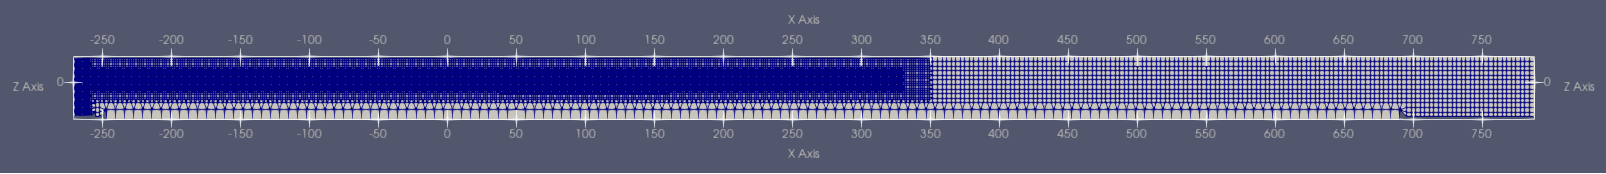
\includegraphics[width=\linewidth]{figures/Validation/grid_naked.png}
    \caption{Complete grid}
    \label{fig:complete grid}
\end{figure}
\begin{figure}[H]
    \centering
    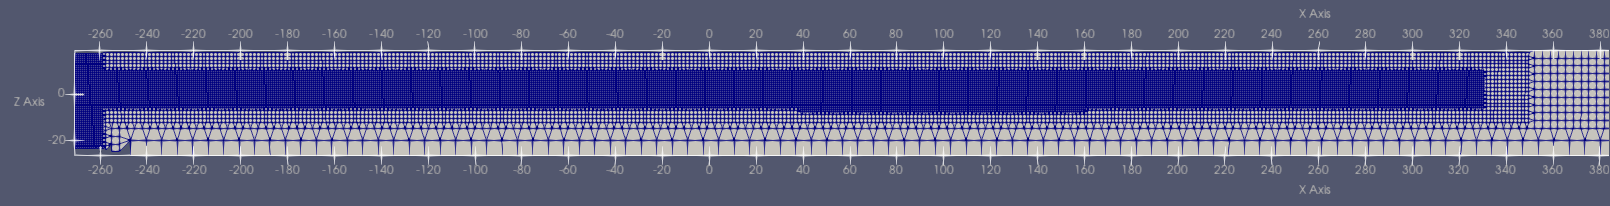
\includegraphics[width=\linewidth]{figures/Validation/grid_zoomed.png}
    \caption{Grid, zoomed on refinement}
    \label{fig:zoomed grid}
\end{figure}


Within this general outline, different refinements have been tested to obtain the optimal refinement. The different grid refinements are numbered from one to five and their characteristics are shown in Table \ref{tab:celldimensions}. The \textit{computation time} is the execution time of ComFLOW of one simulation of 250 seconds.

% Please add the following required packages to your document preamble:
% \usepackage{booktabs}
\begin{table}[H]
\centering
    \begin{tabular}{@{}ccccc@{}}
    \toprule
    grid number & finest cell width {[}mm{]} & finest cell height {[}mm{]} & number of cells & computation time \\ \midrule
    1           & 125                 & 125                  & 5.429.720 & 4 days \\
    2           & 250                 & 250                  & 1.486.840 & 13 hours \\
    3           & 500                 & 500                  & 442.420 & 2 hours \\
    4           & 825                 & 830                  & 209.600 & 1 hour \\ 
    5           & 1250                 & 1250                & 113.440 & 15 minutes  \\ \bottomrule
    \end{tabular}
    \caption{Grid properties}
    \label{tab:celldimensions}
\end{table}



% \subsection{orthogonality}
% \subsection{skewwness}

\section{Propagation of free surface waves}
\label{sec: prop of free surface waves}
%wave only
%Numerical dissipation \& reflection at boundary
%dissipation means high frequency components get smoothed out. Lower frequency oscillations damp at a much slower rate! 
%numerical dissipation iss not suposed to be in the behaviour of the original equations, but is introduced by using numerical approximations. 
%since first-order approximations cut off higher order terms, numerical dissipation occcurs when the higher harmonics are present, higher harmonics tend to have large excitations with small perturbations (since they scale with at least the x^2), so when time step or dimensional step gets large numerical dissipation will be large


The propagation of free surface waves is studied by simulating waves in grids alone, without the interference of any geometry. \textbf{For all simulations, including those in the following sections, 250 seconds of a regular wave was generated with the following characteristics: H = 0.5 m and T = 10.4 s}. The choice for such a long and shallow wave has been made to minimise the nonlinear terms present, in order to allow comparison with linear wave theories, which is elaborated more in Section \ref{sec: box-type breakwater}.\\
\\
Figure \ref{fig:averagewaveheight} shows the average wave height over the refined domain (-270m < x < 350m).  How this is determined is as follows; from each position in the domain, the average wave height is taken from the moment the waves are fully developed in the entire refined domain. Therefore, the time signal on the right side of the refined part of the domain (x = 350 m) is taken (see Figure \ref{fig:waterelevation350m}), from which it can be concluded that the first 125 seconds of simulation is the ramp up time. So, for every position along the x-direction of the domain the first 125 seconds of simulation is discarded, and a mean value of the wave height is determined. This is plotted over the entire length of the refined domain and results in Figure \ref{fig:averagewaveheight}. To see the percentage in which the average wave height varies over the domain, the y-axis of the graph is normalised with the height of the incoming wave.  


\begin{figure}[H]
     \centering
     \begin{subfigure}[b]{0.49\textwidth}
         \centering
         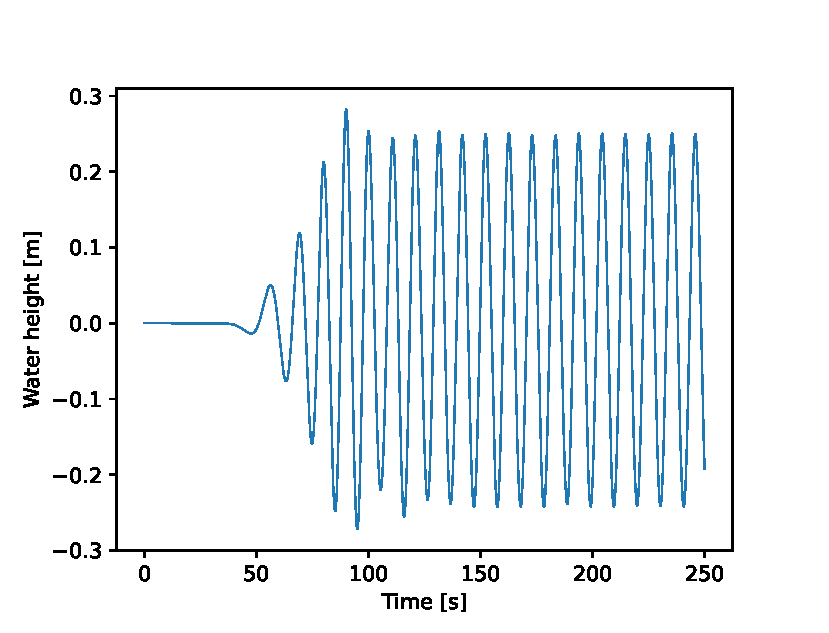
\includegraphics[width=\textwidth]{figures/Validation/water_elevation_350m_eps.eps}
        \caption{Water elevation at x = 350 m}
        \label{fig:waterelevation350m}
     \end{subfigure}
     \hfill
     \begin{subfigure}[b]{0.49\textwidth}
         \centering
        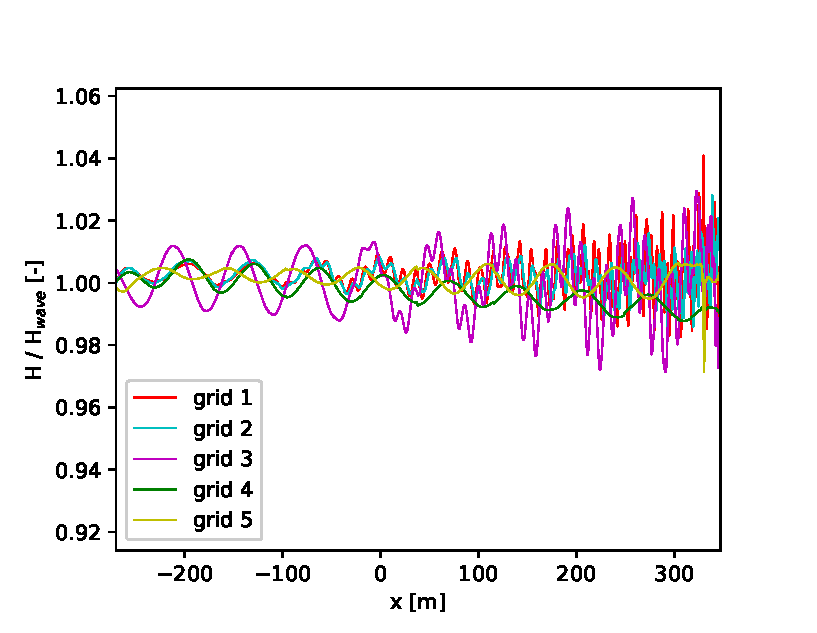
\includegraphics[width = \linewidth]{figures/Validation/numerical_dissipation_eps.eps}
        \caption{Average wave height over length grid}
        \label{fig:averagewaveheight}
     \end{subfigure}
     \caption{Water elevation over time and average wave height over the grid}
\end{figure}


% \begin{figure}
%     \centering
%     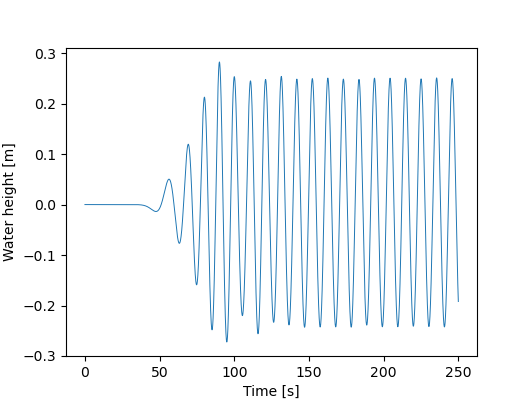
\includegraphics[width=\linewidth]{figures/Validation/water_elevation_350m.png}
%     \caption{Water elevation at x = 350 m}
%     \label{fig:waterelevation350m}
% \end{figure}


% % -general outline is determined by studying the numerical dissipation. And eventual result is: PICTURE OF OUTLINE OF GRID, WITH DIFFERENT REGIONS AND EXPLAIN THE REGIONS
% % -average wave height determination calculation\\
% % -- not going to show 100.000 plots of all the simulations, but to give an insight in the progression, the numerical dissipation first looked like this (few or one example)
% % -- eventually, looked like this: with grid (refinement not clear yet). 

% \begin{figure}[H]
%     \centering
%     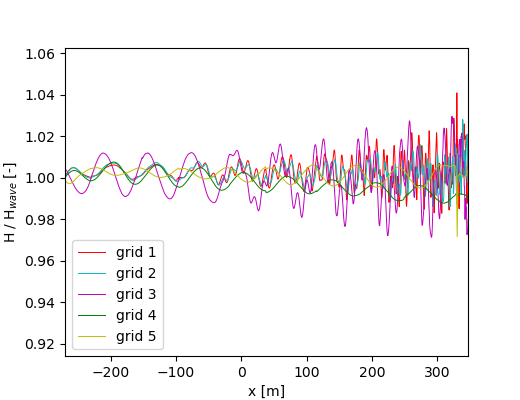
\includegraphics[width = \linewidth]{figures/Validation/numerical_dissipation.png}
%     \caption{Average wave height over length grid}
%     \label{fig:averagewaveheight}
% \end{figure}

What is interesting to note is that the coarse grids give good results in terms of reflection because they vary within 1\% of the incident wave height. There is a pattern of standing waves, which is the result of some of the wave energy reflecting off the outer boundary of the grid or at the refinement level edges. The finer grids, on the other hand, give oscillating results. The small y-axis limits are a bit misleading because the average wave height along the domain still varies within three per cent for the worst grid. 

% \textcolor{red}{It is not yet clear why the fine grids behave this way and a solution is currently being sought.} \\
The numerical dissipation that takes place over the length of the grid is better for fine grids. Especially in grid 5, the average wave height decreases in height as x increases, which means that the wave energy is lost through numerical dissipation as the wave propagates through the domain. 



\section{Wave interaction with a box-type breakwater}
\label{sec: box-type breakwater}
%box type
%Reflection
How ComFLOW deals with the reflection, transmission, and dissipation of wave energy when a box-shaped
structure interacts with regular waves is studied in this section. The comparison with the analytical formula for the transmission coefficient derived by \citet{macagno1953fluid} is made in Section \ref{subsec: Macagno formula}. The mean wave drift force acting on the structure is compared to the analytical mean wave drift force derived by \parencite{longuethiggins1977}, in Section \ref{subsec: driftforces}. Both analytical formulas are derived by linear wave theory, so a long and shallow wave is simulated (H=0.5m and T=10.4s), to minimise the non-linear terms in the simulated waves. In this way a fair comparison can be made with the analytical formulas. \\
\\
For all grids, simulations are done with a box-type structure, with a varying width from 10 to 100 metres and a draught of 5 metres. It is placed in the grid in such a way that the right side of the box is always placed at x = 150 m. 

% -reflection is validated by the Macagno formula and the forces experienced.\\
% -explain relevance of Macagno formula and forces. Results compared with analytical values. A long and shallow wave (H=0.5 with T=10.4) is tested to reduce nonlinear effects.


\subsection{Macagno formula}
\label{subsec: Macagno formula}
The transmission coefficient $K_t$, which is the ratio between the transmitted wave height $H_t$ and the incident wave height $H_i$, is derived by \citet{macagno1953fluid} with linear wave theory.
% \begin{equation}
%     K_{\mathrm{t}}=\frac{1}{\sqrt{1+\left[\frac{k W_{\mathrm{f}} \sinh (k h)}{2 \cosh \left(k h-k T_{\mathrm{f}}\right)}\right]^{2}}}
%     \label{eq: macagno1953}
% \end{equation}


To compare these results to ComFLOW, the transmission coefficient $K_t = H_t / H_i$, the reflection coefficient $K_r = H_r / H_i$ and the dissipation coefficient $K_d$ are determined. The incident wave height $H_i$ is input (in this case: 0.5 metres), so only the transmitted wave height $H_t$ and the reflected wave height $H_r$ must be derived. The latter two can be used to quantify the loss/dissipation coefficient $K_d$.\\
\\
The \textbf{transmitted wave height $H_t$} is derived by averaging the mean wave height after the geometry. This is done in the same way as has been done for the wave-only cases discussed in Section \ref{sec: prop of free surface waves}, but now only between x = 190 m and x = 260 m. ComFLOW gives as output the water elevation over time for every cell in the x-direction at the waterline (which are 560 cells in total for grid 1). This averaging over 70 metres is convenient because this way the oscillating behaviour observed in Section \ref{sec: prop of free surface waves} is filtered (see Figure \ref{fig:averagewaveheight}). \\
\\
The \textbf{reflected wave height $H_r$} is determined via wave splitting theory according to \citet{Goda1976}, by comparing the time series of the water elevation between two points in front of the box, distancing a quarter of a wavelength from each other. This technique is explained extensively in Appendix \ref{app: wave splitting}.\\
\\
Now $H_i$,$H_t$ and $H_r$ are known, the \textbf{dissipation coefficient $K_d$} can be determined via the following derivation.
\begin{equation}
    H_t^2+H_r^2+H_d^2=H_i^2
\end{equation}
\begin{equation}
    K_d = \sqrt{1-K_t^2-K_r^2}
\end{equation}




\begin{figure}[h]
    \centering
    \begin{subfigure}[b]{0.49\textwidth}
        \centering
        \includegraphics[width=\textwidth]{figures/Validation/magagno_with_grid_simulations_eps.eps}
        \caption[]%
        {{\small Transmission, reflection and dissipation coefficient as function of floater width for all grids compared with the Macagno formula}}    
        \label{fig:Macagnocomparison}
    \end{subfigure}
    \hfill
    \begin{subfigure}[b]{0.49\textwidth}  
        \centering 
        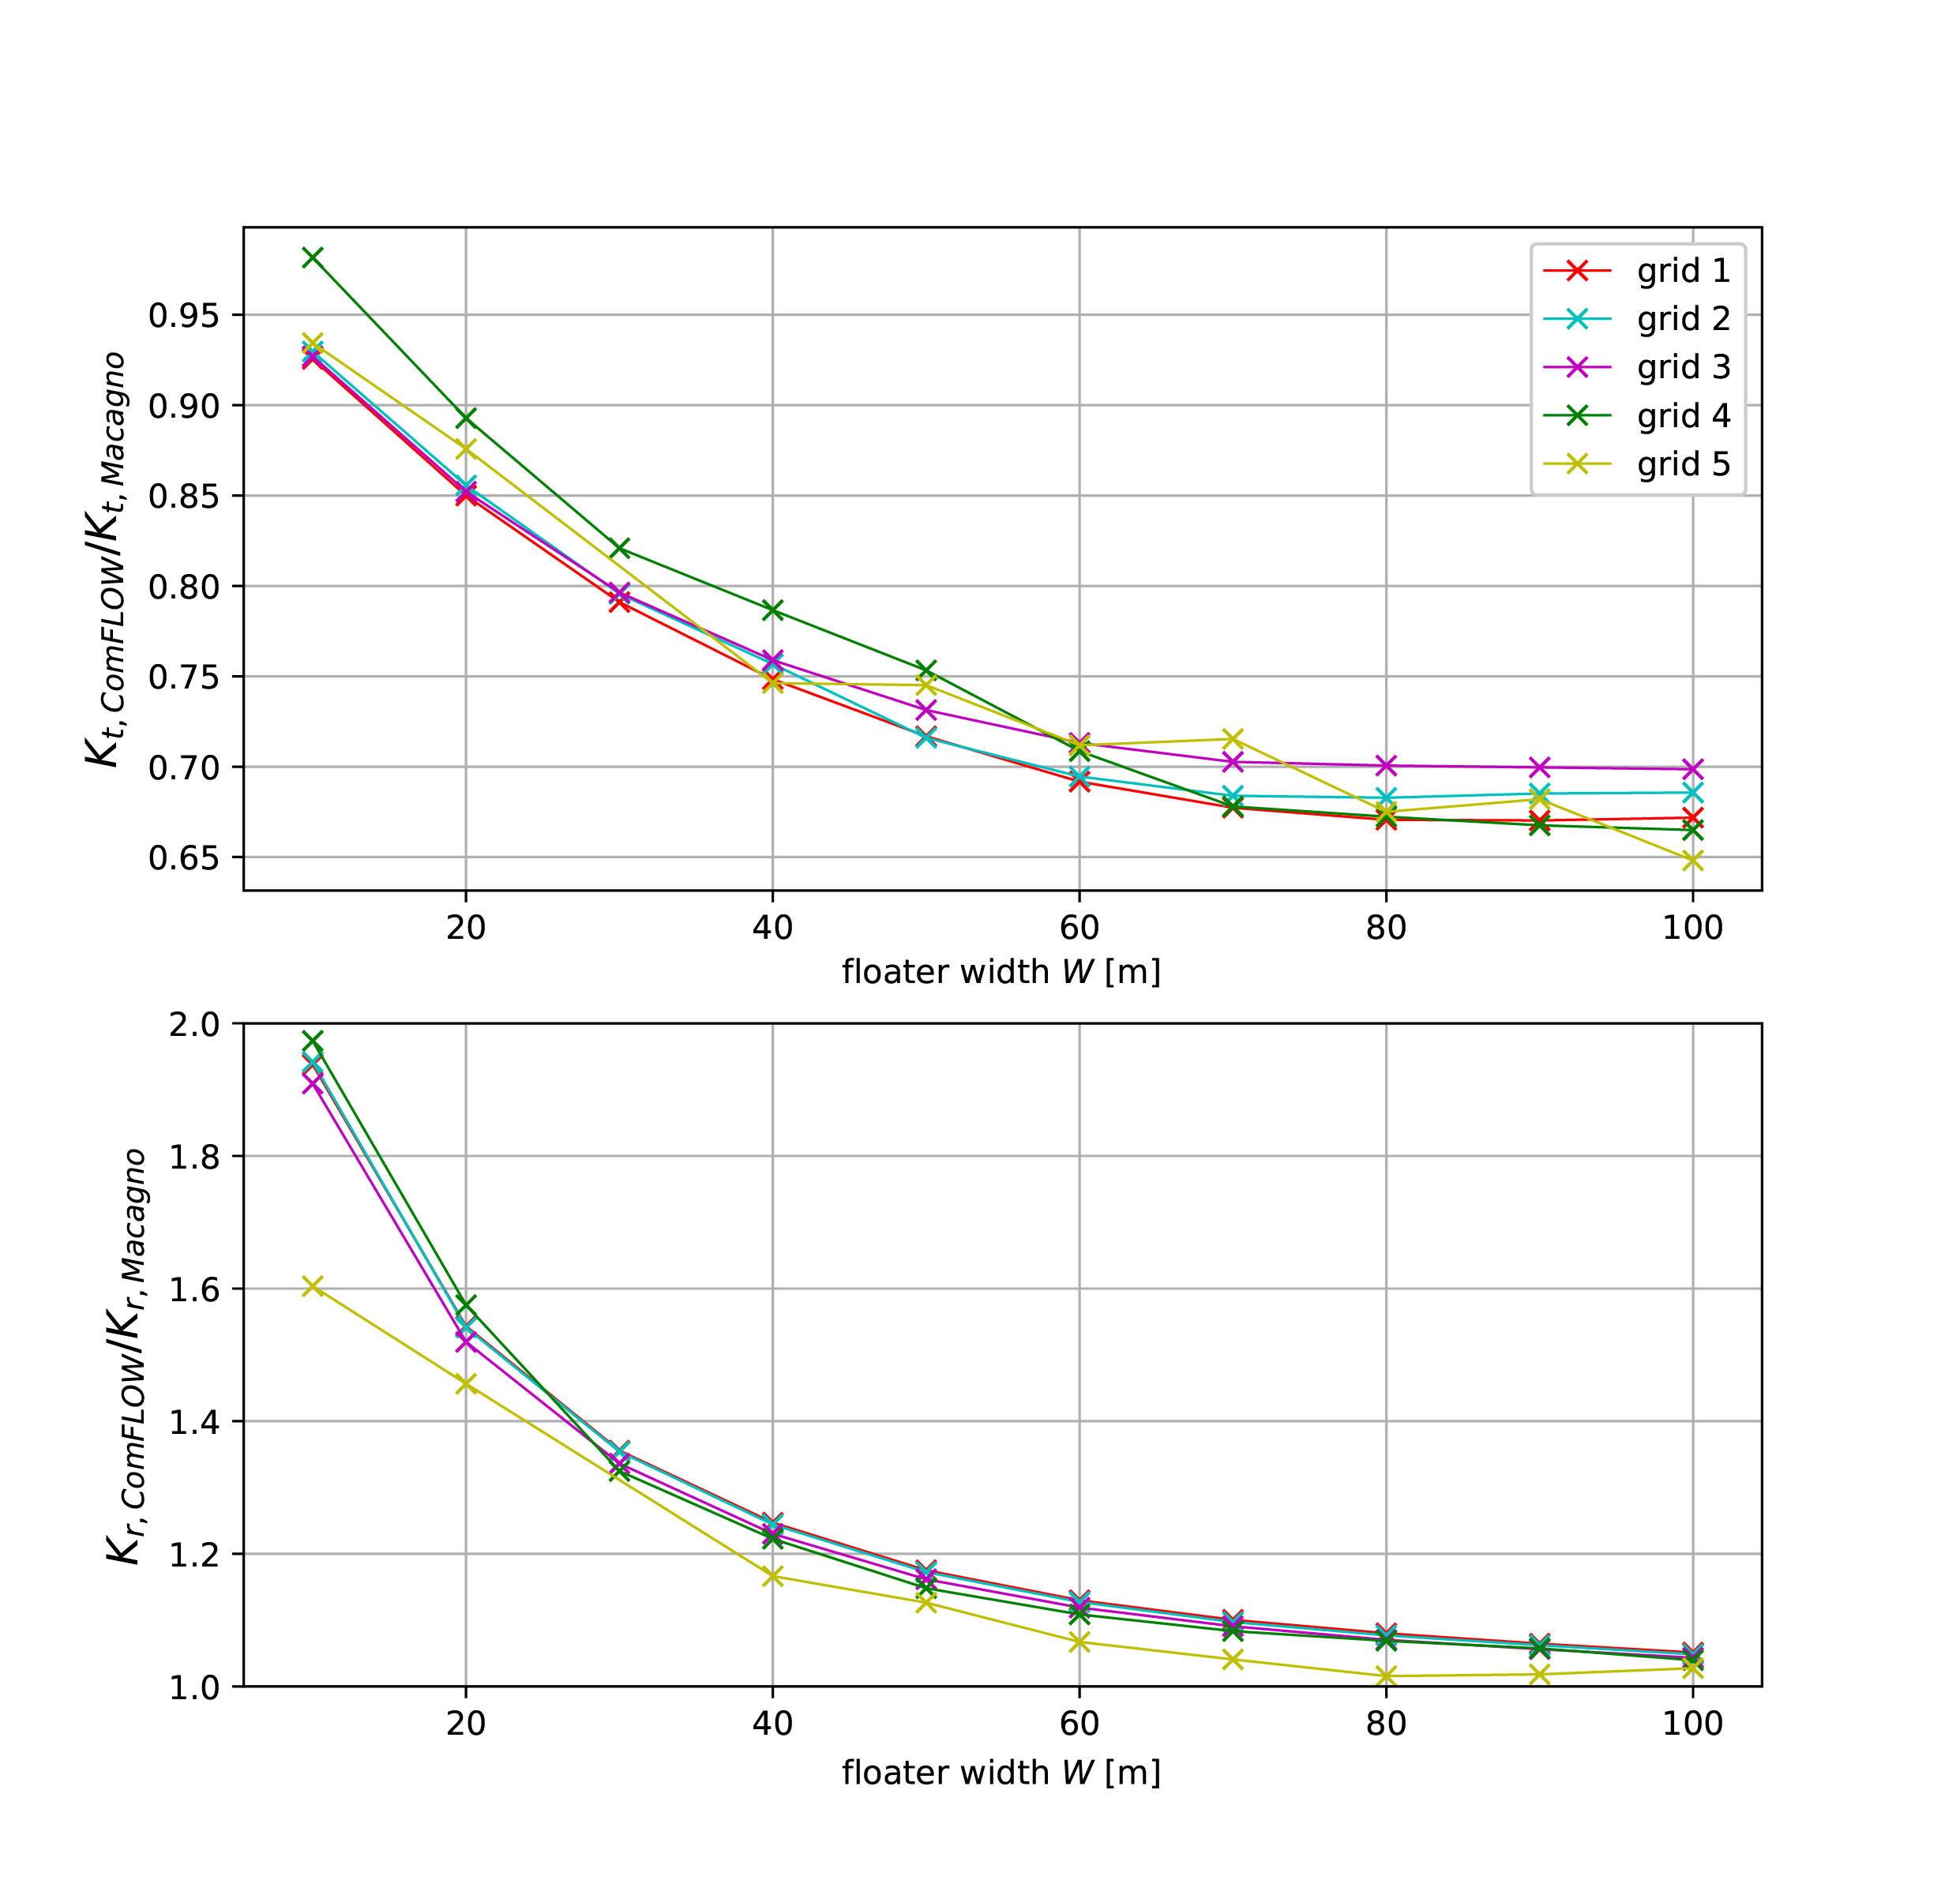
\includegraphics[width=\textwidth]{figures/Validation/magagno_offset_eps.png}
        \caption[]%
        {{\small Offset between ComFLOW results and linear wave theory}}    
        \label{fig:offset macagno}
    \end{subfigure}
    
    \caption{}
    \label{fig: }
\end{figure}

The results of ComFLOW, compared to the analytical Macagno formula, are plotted in Figure \ref{fig:Macagnocomparison}. 
The upper plot shows the transmission coefficient $K_t$. All grids, except grid 4, seem to converge to a static value in this plot. This static value follows the same trend as the analytical formula, but has an offset. Apparently, the transmitted wave height in ComFLOW is smaller than the transmitted wave height according to linear wave theory. What has been found is that if higher, steeper waves were simulated (i.e. nonlinearity increases), this difference in the analytical formula increases. So, this offset can be an indication that non-linearities are still present in the simulated waves. Also, this difference seems to get bigger while the box gets wider, which is an indication that nonlinearities are more dominant with a wider box.\\

The reflection coefficient $K_r$ is derived analytically from the Macagno formula (equation \ref{eq: macagno1953}) and $K_r^2 = 1 - K_t^2$. Here, the same effect is observed. The reflected wave height $H_r$ is observed to be larger in ComFLOW than according to linear wave theory, but this effect decreases as the box width increases. All grids except grid 5 seem to have converged to a static value in this plot.\\

% \begin{equation}
%     K_r = \sqrt{1 - K_t^2}
% \end{equation}


The lower plot shows the dissipation coefficient. Here, grids 4 and 5 give unrealistic results. Grids 1 and 2 have converged to a static value of around 0.1. This means that 10\% of the incoming wave height is dissipated by the presence of the box-type structure. Also, grid 3 is pretty close to convergence. \\
\\




In Figure \ref{fig:offset macagno} the offset is quantified. The upper plot shows that the difference in transmission coefficient $K_t$ between the ComFLOW results and the linear wave theory is 7\% for small widths and increases to 32\% for large box widths.
The reflection coefficient goes from 0.22 to 0.42, which is an increase of 91\% for the smallest box width simulated (W=10 m), but this increase increases to 4\% for the widest floaters. 
So, for short breakwaters, ComFLOW is more reflective, and for long breakwaters, ComFLOW is more dissipative than the Macagno formulation. 
% The results are plotted in Figure \ref{fig:Macagnocomparison}. With $K_t$ and $K_r$ as depending of the box width, grid 1 to 4 seem to converge to a constant solution, with an offset from the analytical formulas. The reflected wave height seems to be higher in the simulations and therefore, the transmitted wave height is lower as well. The lower plot shows the amount of dissipation as function of the width of the box. Grid 1 and 2 converged to each other from a box width greater than 50 meters. 

\subsection{Check other influences}

\subsubsection{Influence coarse grid near the bottom}
Since the coarse grid near the bottom covers a large part of the grid, a check is made to investigate whether its presence has any influence on the results. Therefore, four different floater widths \textit{W} are simulated and analysed. Figure \ref{fig:check coarse bottom} shows that the presence of the coarse grid near the bottom has no influence on the result of the transmission coefficient, so this is beneficial to keep it in future simulations.
% \begin{figure}[H]
%     \centering
%     \includegraphics[width=0.7\linewidth]{figures/Validation/magagno_investigation_fine_bottom.eps}
%     \caption{Investigation whether coarse bottom has a negative influence}
%     \label{fig:check coarse bottom}
% \end{figure}


% \subsubsection{Influence different ka}
% \begin{figure}[H]
%     \centering
%     \includegraphics[width=0.7\linewidth]{figures/Validation/magagno_investigation_different_kas.eps}
%     \caption{Influence of different wave steepnesses ka}
%     \label{fig:my_label}
% \end{figure}

\subsubsection{Influence different wave periods}
Different wave periods were also tested and compared to linear wave theory and resulted in similar percentage offsets. 
% \begin{figure}[H]
%     \centering
%     \includegraphics[width=0.7\linewidth]{figures/Validation/magagno_investigation_different_waveperiods.eps}
%     \caption{Different wave period compared to the Macagno formula}
%     \label{fig:different wave period check on macagno}
% \end{figure}



\begin{figure}[H]
    \centering
    \begin{subfigure}[b]{0.49\textwidth}
        \centering
        \includegraphics[width=\textwidth]{figures/Validation/magagno_investigation_fine_bottom.eps}
        \caption[]%
        {{\small}Investigation whether a coarse grid near the bottom has a negative influence}    
        \label{fig:check coarse bottom}
    \end{subfigure}
    \hfill
    \begin{subfigure}[b]{0.49\textwidth}  
        \centering 
        \includegraphics[width=\textwidth]{figures/Validation/magagno_investigation_different_waveperiods.eps}
        \caption[]%
        {{\small}Different wave period compared to the Macagno formula}    
        \label{fig:check different periods macagno}
    \end{subfigure}

    
    \caption{}
    \label{}
\end{figure}



\subsection{Drift forces}
\label{subsec: driftforces}
The forces in ComFLOW are determined by integrating the pressure over the surface of the geometry. The first-order wave forces have the same frequency as the wave frequency. The raw output from ComFLOW is subject to high-frequency oscillations due to the rapid pressure fluctuations around the structure. Therefore, all frequencies above twice the wave frequency are filtered out of the signal, resulting in the time series of the total wave force where the first-order component is clearly visible (see Figure \ref{fig:forceovertime}).\\
\begin{figure}[H]
    \centering
    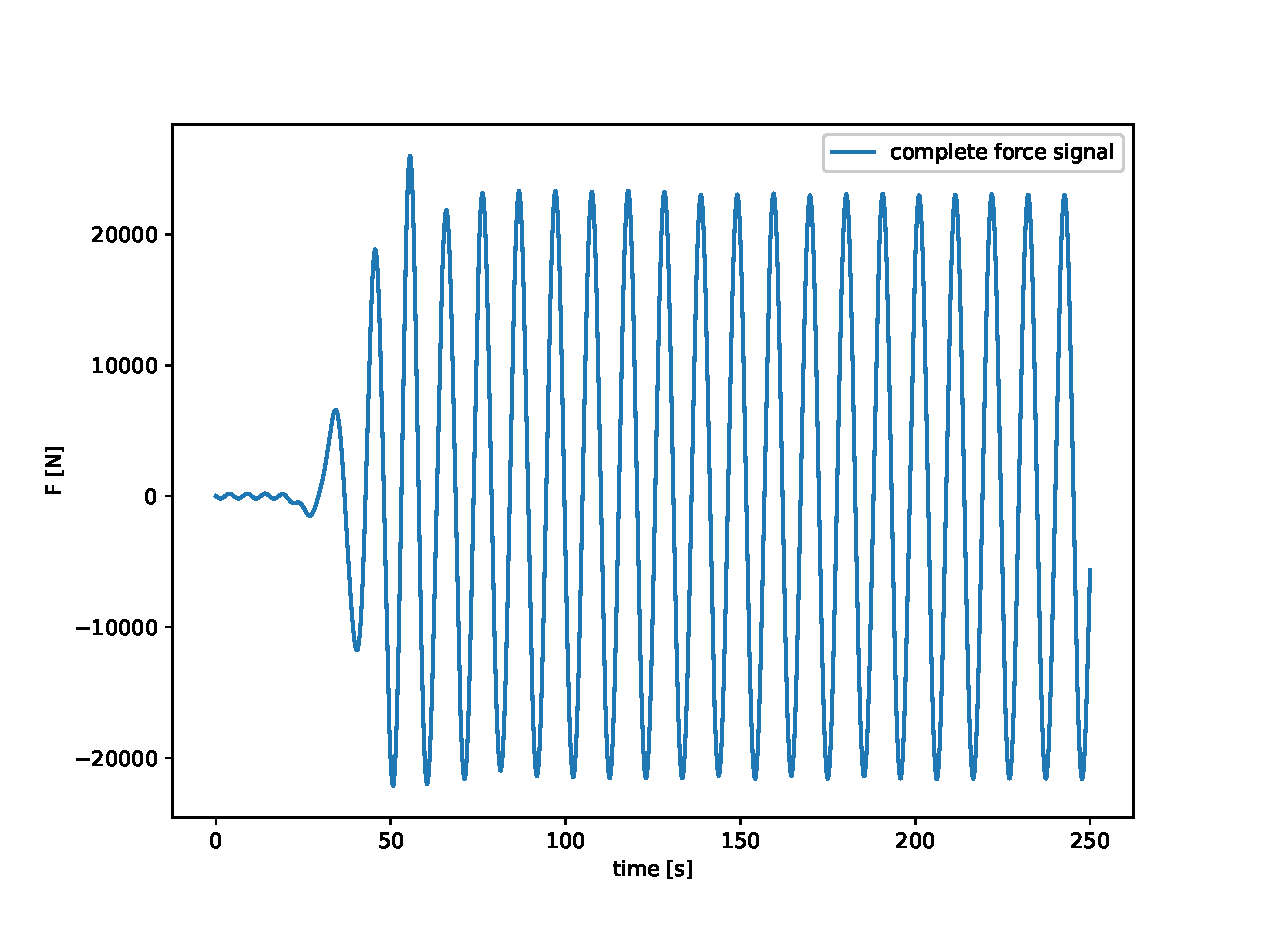
\includegraphics[width=0.6\linewidth]{figures/Validation/forcesignal_on_single_box_eps.eps}
    \caption{Force in x-direction on the box over time}
    \label{fig:forceovertime}
\end{figure}
The filtered signal (in Figure \ref{fig:forceovertime}) was needed by automatically determining when the waves were fully developed and for cutting part of the simulation to reach an integer amount of waves. However, the unfiltered output of ComFLOW is used in the calculation of the mean wave drift force. This is done for different widths of the box, for all grids studied, resulting in a mean wave drift force for each configuration and is compared to the analytical value of the mean wave drift force according to \citet{longuethiggins1977} in Figure \ref{fig:meanforceanalyticalcomparison all grids}. From which it is easily observable, grid 3 t/m 5 gives very unrealistic results. Therefore, they are discarded in Figure \ref{fig:meanforceanalyticalcomparison two grids}.

% \begin{figure}[H]
%     \centering
%     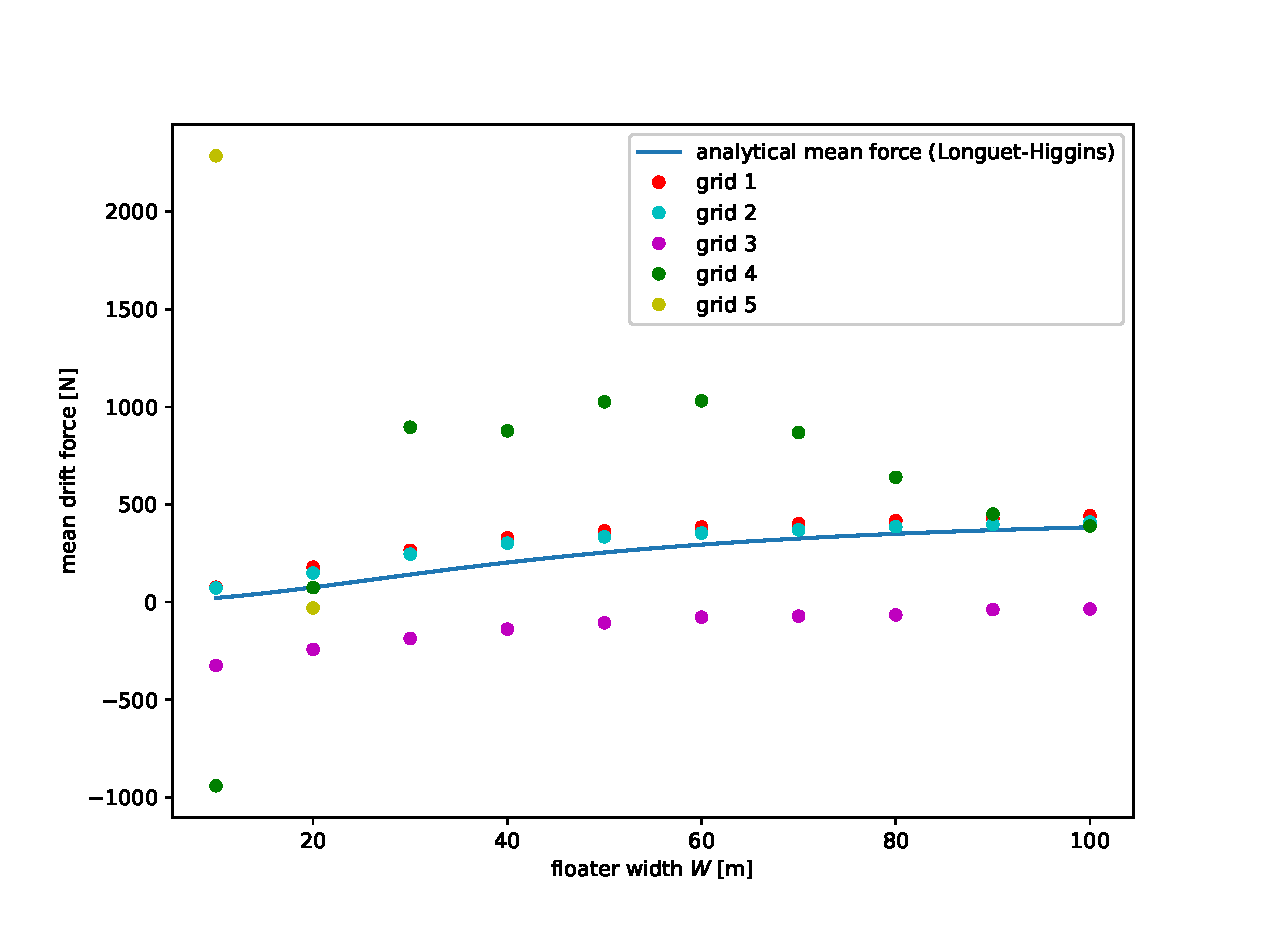
\includegraphics[width=\linewidth]{figures/Validation/forces_with_all_grids.eps}
%     \caption{Mean force on box in x-direction as function of width of the box, all grids}
%     \label{fig:meanforceanalyticalcomparison all grids}
% \end{figure}

In Figure \ref{fig:meanforceanalyticalcomparison two grids} both grids with applicable results (grids 1 \& 2) are shown. As can be seen in Table \ref{tab:celldimensions}, grid 1 took four days to compute, which is disproportionately high for this kind of simulation. Therefore, the results of grid 1 are considered the best ComFLOW can get and are used as a benchmark to determine the optimal grid. Grid 2 converged to this solution, with a small offset. The solid line is the analytical force, where the reflected and transmitted wave height is calculated with the Macagno formula \ref{eq: macagno1953} \parencite{macagno1953fluid} and the force is calculated with equation \ref{eq: longuethiggins force}, derived by \citet{longuethiggins1977}. The dashed lines are also calculated with equation \ref{eq: longuethiggins force}, but with the wave heights determined by the output of the ComFLOW simulations. These dashed lines comply with the force output of ComFLOW, which means that the calculation of the force acting on the structure is very accurate, but the determination of the reflected and transmitted wave height is a bit off. This is an interesting and useful result, as the actual wave height in ComFLOW can be easily determined. Therefore, a qualitative analysis can be done for the drift forces on the structure. In the previous section, the reflected wave height was found to be higher in ComFLOW than according to the linear wave theory (see Figure \ref{fig:Macagnocomparison}). More reflection on the structure results in a higher mean wave drift force (according to equation \ref{eq: longuethiggins force}). Therefore, the greater force found by ComFLOW compared to linear wave theory was expected since the analysis of Section \ref{sec: box-type breakwater}.


% %difference in results are clearly not from the calculation of the forces, but from the numerical dissipation? not sure though?
% \begin{equation}
% F=\frac{1}{4} \rho g\left(a_i^{2}+a_r^{2}-a_t^{2}\right)(1+ \frac{2 k h}{\sinh 2 k h})
% \label{eq: force longuet}
% \end{equation}

% \begin{figure}[H]
%     \centering
%     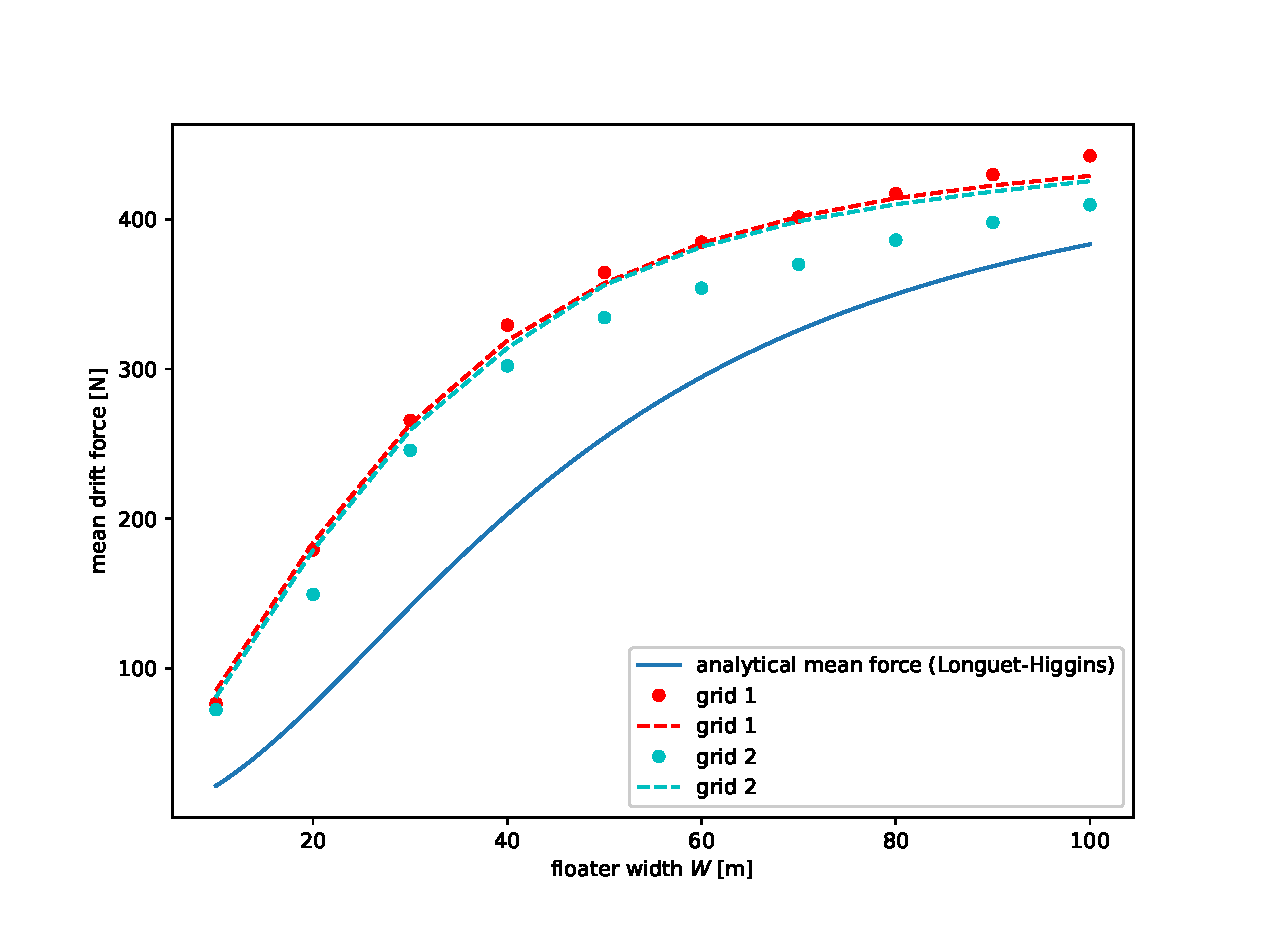
\includegraphics[width=\linewidth]{figures/Validation/forces_with_two_grids_inc_semi_analytical_eps.eps}
%     \caption{Mean force on box in x-direction as function of width of the box, two finest grids}
%     \label{fig:meanforceanalyticalcomparison two grids}
% \end{figure}

\begin{figure}[H]
    \centering
    \hfill
    \begin{subfigure}[b]{0.49\textwidth}  
        \centering 
        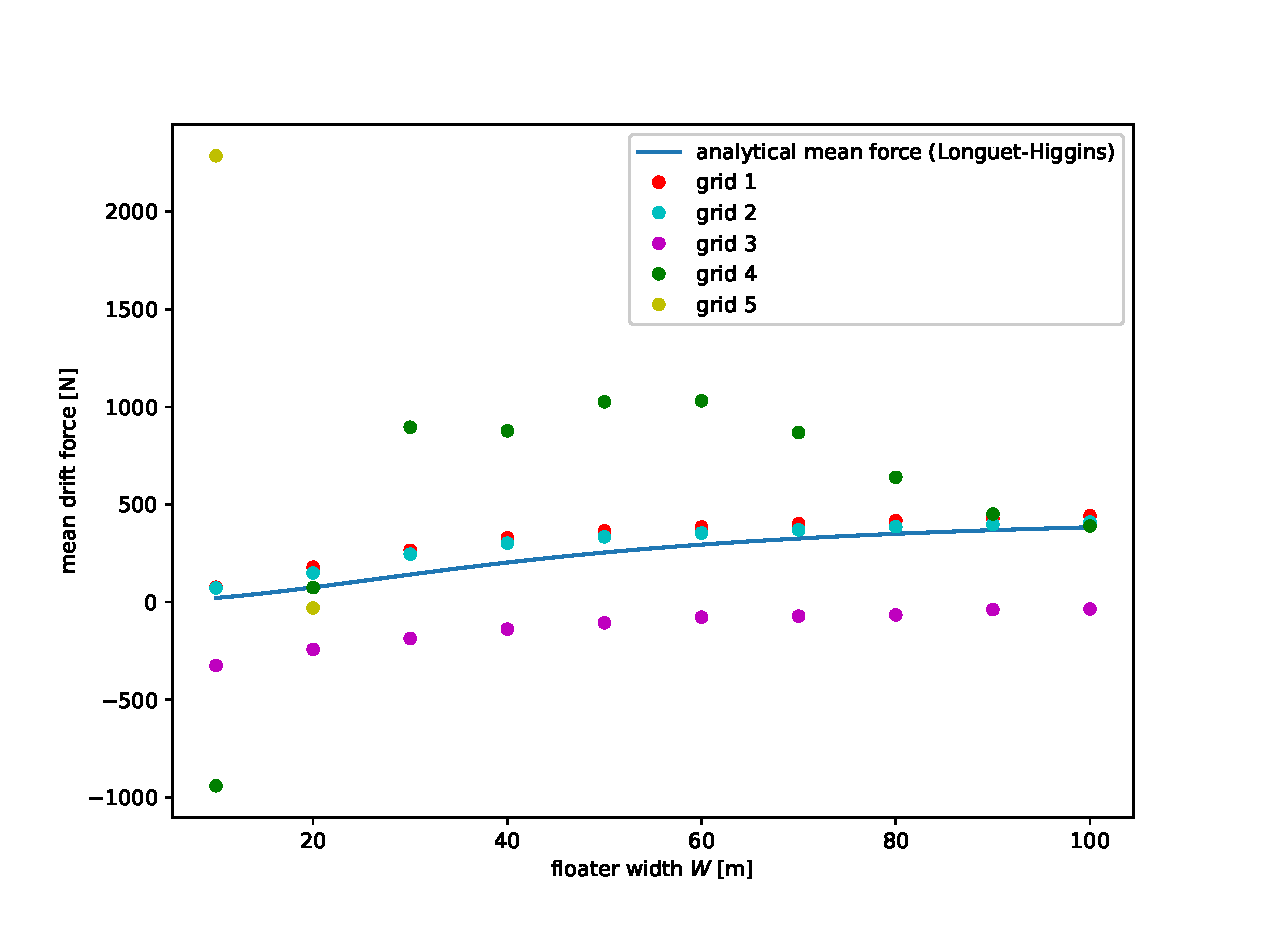
\includegraphics[width=\textwidth]{figures/Validation/forces_with_all_grids.eps}
          \caption[]%
        {{\small}Mean force on box in x-direction as function of width of the box, all grids} 
        \label{fig:meanforceanalyticalcomparison all grids}
    \end{subfigure}
    \hfill
    \begin{subfigure}[b]{0.49\textwidth}
        \centering
        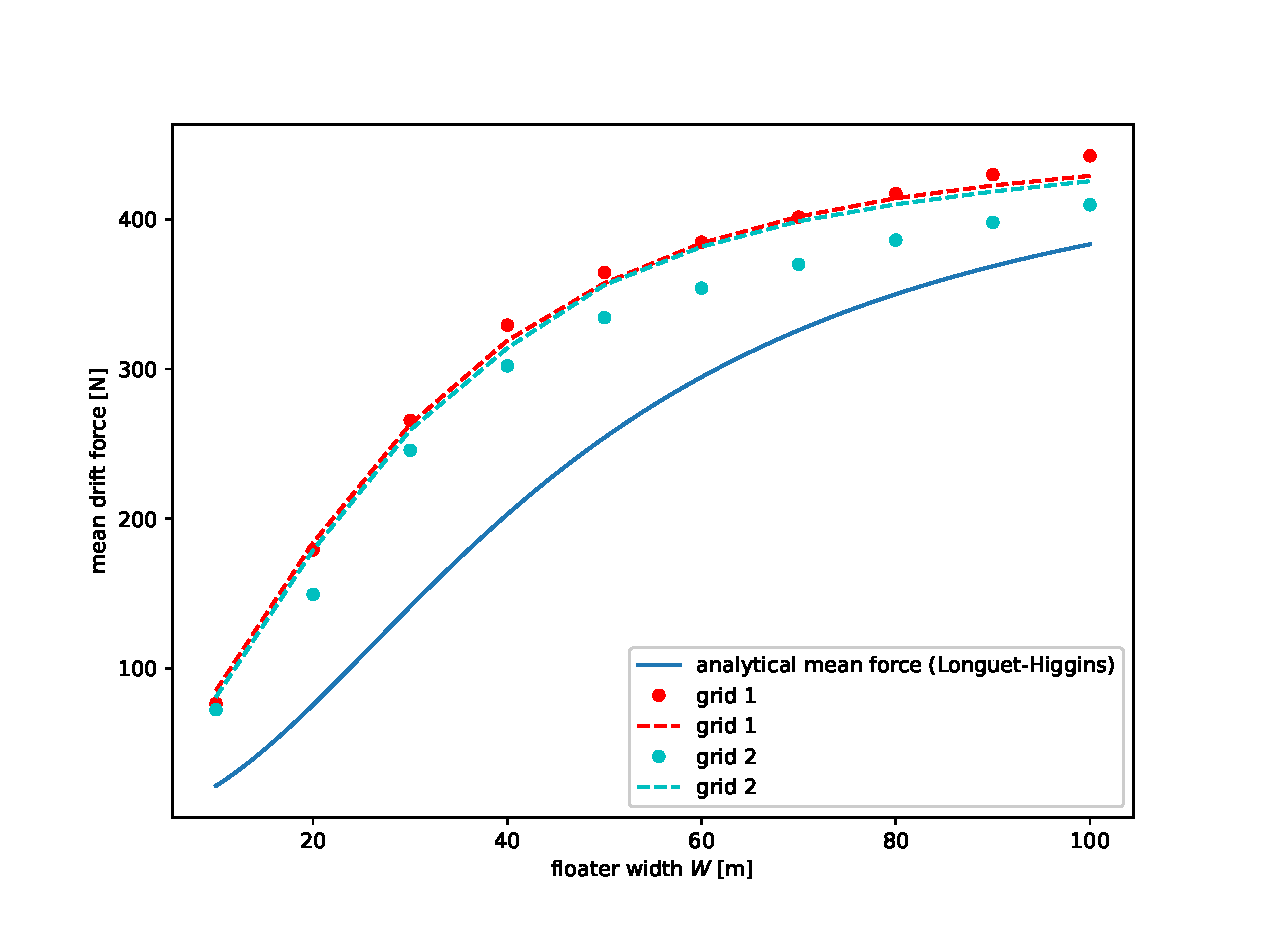
\includegraphics[width=\textwidth]{figures/Validation/forces_with_two_grids_inc_semi_analytical_eps.eps}
        \caption[]%
        {{\small}Mean force on box in x-direction as function of width of the box, two finest grids}    
        \label{fig:meanforceanalyticalcomparison two grids}
    \end{subfigure}
    
    \caption{}
    \label{}
\end{figure}


\section{Energy dissipation through wave breaking}
\label{sec: Dissipation}
%breaker bar
%-An experiment with a breaker bar is mimicked to validate the model on dissipation


As explained in detail in Section \ref{subsec: comflow literature review}, the physical dissipation characteristics in ComFLOW are expected to depend strongly on the grid size in the area where the waves will break. To map this effect, a validation is performed where an experiment, done by  \citet{breakerbarexperiment}, where waves were plunging over a breaker bar, is mimicked in ComFLOW, after which both results were compared. Furthermore, the results of this validation are used to design the correct grid for future simulations by verifying what combination of incident wave height and grid size results in reasonable dissipation rates when waves break.

\subsection{Experiment breaker bar}
A large-scale wave flume experiment has been carried by \citet{breakerbarexperiment} out involving a T = 4s regular wave with H = 0.78 m wave height plunging over a fixed barred beach profile. In the top plot of Figure \ref{fig:breakerbarexperiment}, the bathymetry of the experiment is shown. The waves were generated by a wave paddle at x = 0 and propagated to the right. Elevations of the surface of the water were measured with resistive wave gauges mounted on the side wall at 19 locations along the flume, from x=12 m in the constant depth section of the flume to x=49 m in the shoaling zone. Resistive wave gauges were not deployed in the surf zone since they suffered from spurious measurements due to the strong splash-up of water. For the remainder of the profile, pressure transducers (STS-ATM/N) were therefore fitted along the flume sidewall at an approximate 0.5 m spacing. The elevations of the water surface were retrieved from the pressure measurements after correction for pressure attenuation due to depth using linear wave theory. \\
\\


\subsection{Grid settings}

This experiment has been simulated in ComFLOW, with a uniform grid over the entire domain. The purpose is to give an insight into what settings to use and how fine the grid needs to be around the geometry later on in this project, where wave breaking will occur as well. The exact dimensions of the cell sizes of the different grids are shown in the legend from Figure \ref{fig:breakerbarexperiment}. 



% -to find the optimal grid refinement for around the geometry where the dissipation occurs, an experiment is compared with ComFLOW results.
%  -show the effect of breaking on convection scheme (refer to paragraph: convection scheme, in chapter settings)
% -standing wave pattern as expected, difficult to measure wave height when breaking (liquid fill ratios are used, so when lots of air in wave, unrealistic values), doesn't matter, as long as $a_i$ and $a_t$ are corresponding and they do.
% %- put some statistics in here, thrustworthy interval, some boxplots on how much the ComFLOW simulations could be trusted

\begin{figure}[H]
    \centering
    \includegraphics[width=0.8\linewidth]{figures/Validation/plot_stats_compare_H-1.eps}
    \caption{Results different grids in ComFLOW with experiment \parencite{breakerbarexperiment}}
    \label{fig:breakerbarexperiment}
\end{figure}


The results show that the wave height behind the breaker bar (58m < x < 63 m) corresponds very well to the experiment for all grids except the one indicated with the orange line in Figure \ref{fig:breakerbarexperiment}. The wave height in front of the breaker bar (x < 50 m) corresponds to the experiment for all grids except the one with cell dimensions with dx and dz of 500 mm. What is interesting to note is that the mean water level (third plot in Figure \ref{fig:breakerbarexperiment}) is generally higher than in the experiment.  Also, ComFLOW does not seem to take the set-down when waves get very steep before breaking into account. \\
The wave height exactly at the breaking point (x = 53m) does not correspond at all to the experiment, and the different grids differ here as well. This is because much air is intruded into the water at the moment of breaking. ComFLOW determines the elevation of water by checking the liquid fill ratios of each cell and adding the amount of water in a vertical column of cells. Therefore, when lots of air is intruded into the water, ComFLOWs results might differ from the actual height of the waves. In addition, measurements of the wave height of a wave with a lot of entrapped air in the experiments are not trivial as well. In other words, the measurements of the experiment at position 50 m < x < 54 m are also not inviolable. For further simulations, this is no problem at all, since only the transmitted wave height, reflected wave height, and incident wave height need to be determined in order to derive the amount of wave energy lost in the breaking process. The difference in wave height between the different grids can also be declared by the difference in numerical dissipation. The green line (with a dx and dz of 500 mm) dissipates the most during shoaling, which is quite logical because this grid is very coarse. \\


\subsection{Convection scheme}
\label{subsec: breakerbar on convection scheme} 
The convection scheme seems to have a significant impact on the breaking characteristic of ComFLOW, which can be seen in Figure \ref{fig:breakerbarexperiment convection scheme}. Here, both convection schemes (first-order upwind and second-order central) have been simulated with the same grid, with cell size: dx = 50mm and dz = 25mm. The second-order central convection scheme gave less favourable results than the first-order upwind scheme. The wave height after the breaker bar differs more from the experiment's measurements (see Figure below). Furthermore, the second-order central convection scheme resulted in very high local fluid velocities in the breaking process. Thus, the time step per computation will be high, which results in unreasonably large execution times.\\
\\
This poor behaviour of the second-order central method might be due to the fact that this method uses three cells in order to do one discretization (see SubSection \textbf{Convection scheme} of Section \ref{subsec: numercial settings validation}), while the first-order upwind method uses two cells. Since the breaking process takes place around the water line and tiny air pockets get entrained in the water as well during breaking, the discretization must deal with these two mediums in the flow at a low-dimensional scale. Therefore, it might be too much to accurately do a discretization using three cells. So, although second-order discretizations tend to be more accurate in general, because they take into account second-order terms, this is not the case for the simulation of breaking waves. 



\begin{figure}[H]
    \centering
    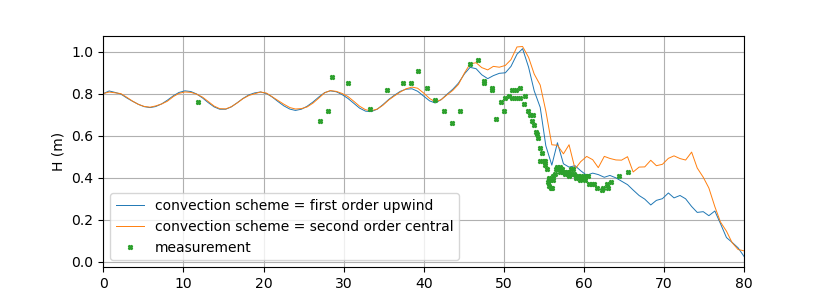
\includegraphics[width=\linewidth]{figures/Validation/plot_stats_compare_H-1_2ndordercentral.png}
    \caption{Influence of convection scheme on breaking characteristics}
    \label{fig:breakerbarexperiment convection scheme}
\end{figure}


% \section{Final settings used in ComFLOW}
% The settings which were found to be best performing are:
% \begin{itemize}
%     \item 
% \end{itemize}

% As mentioned before, the grid dimensions should scale to the properties of the wave. The research in this validation is done with a regular wave with H = 0.5m and T = 10.4s. To make sure the results are applicable to future waves, the cell dimensions of the best performing grid is non-dimensionalized w.r.t. the wave dimensions in the following Table:






%three different HKN waves


\section{Discussion}
The results of ComFLOW were analysed and compared to analytical formulas, and an experiment to make sure its results are reliable and give a good representation of reality. Therefore, the analytical formula for the transmission coefficient: the Macagno formula, derived by \parencite{macagno1953fluid}, and the analytical formula for the mean wave drift force, derived by \parencite{longuethiggins1977}, are compared with the results of ComFLOW by simulating a regular wave of H=0.5 m, T=10.4 s in a water depth of 23 metres for 250 seconds. Furthermore, a fast, but reliable simulation is desired, and therefore the propagation of free surface waves was studied to map the computation time and the numerical dissipation throughout the grid. This also contributes to choosing the right grid for the simulations. Lastly, an experiment where waves were breaking over a breaker bar was mimicked in ComFLOW to compare the experimental outcome with ComFLOWs results. Therefore, the dissipation characteristics of ComFLOW are mapped.
\\
Five different grids were tested, numbered from grid 1 to 5 sorted according to refinement, where grid 1 was the finest and grid 5 the coarsest. Grid 1 took more than four days to compute with its 5 million cells. Grid 2, containing roughly one and a half million cells, converged to the same solutions as grid 1 but took only 13 hours to compute. Grid 3, 4 and 5 gave unreliable results; where the forces resulting from the simulations with these grids were either extremely high or extremely low, sometimes even negative. So, the coarseness of grid 2 is labelled as best for the simulation with a regular wave with characteristics: H=0.5 m and T=10.4 s. Therefore, since grid 2 has a cell height and width of 250 mm and the draught of the box-type breakwater is five metres, 20 cells are necessary over the height of the geometry to give reliable forces in the x-direction. Although the grid refinements used lead to a converged result (i.e., independently of further refinements) which follows the same trend as the analytical formulas, it still gives an offset to the analytical formulas corresponding with linear wave theory. The transmitted wave height measured in the simulations with ComFLOW was too low, and the reflected wave heights were too high. The mean wave drift forces were also a bit too high, which is due to the excessively high reflection coefficient. \\
The comparison with ComFLOW and the experiment in which waves plunged over a breaker bar showed good results. The height of the wave behind the breaker bar matched well for all grids on the grid with dx=200mm and dz=200mm. In other words, the dissipation of wave energy by breaking was well simulated in ComFLOW. The height of the wave at the breaking point and the mean water level did not match the measurements of the experiment.

% %The fist sub-research question can be answered already: what is the quality of ComFLOW and untill what extend can it be used compared to real life situations?
% \textbf{This dashed lines comply with the force output of ComFLOW, which means the calculation of the force acting on the structure is very accurate, but the determination of the reflected and transmitted wave height is a bit off. This is an interesting and usefull result, since the actual wave height in ComFLOW can be determined easily. Therefore, a qualitative analysis can be done for the drift forces on the structure. }


% feedback Peter:
% \textcolor{red}{\textbf{it is not the best possible grid, but the best possible grid that I can buy}}


% %in hoeverre kan je vertrouwen op de ComFLOW dissipatie validatie?
% -shortages of ComFLOW (viscous effects too strong)

% -shortages of regular waves:\\
% Since the continuous contribution of different frequencies in a irregular wave spectrum, the natural period of a floating system will often comply with one of the wave frequencies. This will lead to large excitations (see Figure \ref{fig:largeexcitation_lowfreq} from \parencite{journee2000offshore}) and mooring system forces will be dominated by this effect; its design must account for this. 
% But, with regular waves, it is highly likely this phenomena will not occur.....

%  "Later, higher waves in which the higher harmonics are more dominant can be tested and compared with the results of this section in order to quantify the magnitude of the nonlinear terms of the waves.", from Section \ref{subsec: Macagno formula}. This magnitude is not validated, so this guarantees not it is the same.

% -dissipation depends on fineness grid..
\section{Conclusions}

So the coarseness of grid 2 is labelled as best for the simulation with a regular wave with characteristics: H=0.5 m and T=10.4 s. Therefore, since grid 2 has a cell height and width of 250 mm and the draught of the box-type breakwater is five meters, twenty cells are necessary over the height of the geometry to give reliable forces in the x-direction. \\
\\
ComFLOW's results for the transmission coefficient with a varying box width follow the same trend as expected by the Macagno formula, which is a function derived from linear wave theory. Wave transmission is lower in ComFLOW than in linear wave theory: 7\% for small box widths (W=10 m) and increases to 32\% for large widths (W=100m). Wave reflection is higher: 91\% for the smallest box width and 4\% for the widest floaters. \\
\\
All different grid sizes used in the comparison with the experiment were waves plunged over a breaker bar showed results that were in compliance with the experiment. 

\chapter{Hydrodynamic Design Optimisation}
\label{ch: captive design optimisation}



% \begin{figure}[h]
%     \centering
%     \begin{subfigure}[b]{0.49\textwidth}
%         \centering
%         \includegraphics[width=\textwidth]{}
%         \caption[]%
%         {{\small }}    
%         \label{fig:  }
%     \end{subfigure}
%     \hfill
%     \begin{subfigure}[b]{0.49\textwidth}  
%         \centering 
%         \includegraphics[width=\textwidth]{}
%         \caption[]%
%         {{\small }}    
%         \label{fig:  }
%     \end{subfigure}
%     \vskip\baselineskip
%     \begin{subfigure}[b]{0.49\textwidth}   
%         \centering 
%         \includegraphics[width=\textwidth]{}
%         \caption[]%
%         {{\small }}    
%         \label{fig:  }
%     \end{subfigure}
%     \hfill
%     \begin{subfigure}[b]{0.49\textwidth}   
%         \centering 
%         \includegraphics[width=\textwidth]{}
%         \caption[]%
%         {{\small }}    
%         \label{fig:  }
%     \end{subfigure}
%     \hfill
%     \begin{subfigure}[b]{0.49\textwidth}   
%         \centering 
%         \includegraphics[width=\textwidth]{}
%         \caption[]%
%         {{\small }}    
%         \label{fig:  }
%     \end{subfigure}
%         \hfill
%     \begin{subfigure}[b]{0.49\textwidth}   
%         \centering 
%         \includegraphics[width=\textwidth]{}
%         \caption[]%
%         {{\small }}    
%         \label{fig:  }
%     \end{subfigure}
    
%     \caption{}
%     \label{fig: }
% \end{figure}

In this chapter, an optimisation of the design of a breakwater geometry for a captive set-up is presented. A 'captive' setup means that all motions of the structure are restrained. The performance of each breakwater is determined in ComFLOW for 300 seconds simulation time. The first design iteration of the optimisation is performed for Wave Condition 1 (regular waves of H = 3.0 m and T = 6.0 s) and is discussed in Section \ref{sec: design iteration 1 captive}. The results are used to do a second design iteration with boundaries around the optimum of the first design iteration; this is addressed in Section \ref{sec: design iteration 2 captive}. The effect of Wave Condition 2 on the optimal designs is shown in Section \ref{sec: WC2 captive}. Here, the performance of the breakwaters is tested for extreme, regular waves with a height of 9 metres and a peak period of 10.4 seconds. Finally, a more extensive analysis of the results is performed in the final section: \ref{sec: discussion hydrodynamical optimisation}, where an explanation of the results is further analysed based on physical phenomena and the literature. 


% An optimisation based on costs is done in the sections \ref{sec: economical DI1 H3} and \ref{sec: economical DI2 H3} for Wave Condition 1. Finally, the results of the captive design optimisation are discussed in Section \ref{sec: discussion captive design optimization} and conclusions are drawn in Section \ref{sec: conclusions captive design optimization}.
%and sometimes two design iterations are necessary to deliver the optimal design




\section{Design Iteration 1}
\label{sec: design iteration 1 captive}

The first design iteration of the captive set-up is addressed in this section. In Section \ref{sec: DI1 captive H3 approach} the approach is declared, the performance of all the breakwaters in the design space is discussed in Section \ref{sec: DI1 captive H3 performance bw}, in Section \ref{sec: DI1 captive H3 correlation} the correlation between input factors and responses are discussed in Section \ref{sec: DI1 captive H3 response surfaces} the response surfaces are shown, which are used to arrive at the final design optima, which are reported in the final section; \ref{sec: DI1 captive H3 design optima}.


\subsection{Approach}
\label{sec: DI1 captive H3 approach}

In the first design iteration, various configurations of breakwaters are simulated in ComFLOW with varying factors. The limits of these factors are shown in Table \ref{tab: boundaries DI1 captive}. A clarification on how these factors define the actual geometry of the breakwater is explained in Section \ref{subsec: methodology parametrisation} of the \nameref{ch: methodolgy} chapter and visualised in Figure \ref{fig: parametrisation breakwater}. Also, a minimal clearing of 10 metres between the seabed and the bottom of the breakwater is implemented in Design Expert (i.e. the maximum draught is 13 metres, because the water depth is 23 metres), otherwise large fluid velocities below the breakwater were expected, that result in low pressure fields and long execution times. A cubic relation between all the different input parametres and the two responses: the mean drift force and the transmitted wave height, is assumed. To be able to construct the response surfaces, 94 configurations are necessary to be simulated in ComFLOW. With the help of \acrfull{doe} a design space is created, which defines the shape of the 94 configurations. The complete design space is given in Appendix Table \ref{tab: params design iteration 1 captive setup}. To show the variety of the possible geometries of the breakwaters, the parametres for six different configurations are shown in Table \ref{tab: params design iteration 1 captive br 1to6} and are visualised in Figure  \ref{fig:Configurations 1to6 DI1 captive}. Evidently, the breakwaters vary from small wedges completely submerged to big boxes on the surface. 

\begin{table}[h]
\centering
\scalebox{0.65}{
\begin{tabular}{@{}ccccc@{}}
\toprule
Factor & Name        & Units        & Minimum & Maximum       \\ \midrule
A & T               & m & 2.50   & 13.00   \\
B & W               & m & 10.00  & 150.00   \\
C & front\_fraction & - & 0.01 & 0.99  \\
D & top\_fraction   & - & 0.01 & 0.99  \\
E & radius          & m & 500.00 & 2000.00 \\
F & WL              & m & -6.10  & 4.00     \\ \bottomrule
\end{tabular}
}
\caption{Boundaries Design Space Captive Design Iteration 1}
\label{tab: boundaries DI1 captive}
\end{table}

% Please add the following required packages to your document preamble:
% \usepackage{booktabs}
\begin{table}[h]
\centering
\scalebox{0.65}{
\begin{tabular}{@{}ccccccc@{}}
\toprule
configuration & T        & W        & front\_fraction & top\_fraction & radius   & WL       \\ \midrule
16 & 9.59 & 150.00      & 0.01   & 0.01   & 2000.00   & 3.41 \\
24 & 5.44     & 89.80     & 0.01   & 0.2795 & 1985.00   & -3.37   \\
32 & 8.64   & 10.00       & 0.01   & 0.01   & 500.00    & 4.00        \\
37 & 12.30 & 150.00      & 0.85 & 0.5539 & 920.00    & -0.70 \\
40 & 7.75     & 41.16 & 0.99   & 0.79 & 852.50  & -2.87   \\
45 & 2.50      & 150.00      & 0.64 & 0.99   & 1272.5 & 2.18    \\ \bottomrule
\end{tabular}
}
\caption{Parametres breakwater of six different configurations of design iteration 1}
\label{tab: params design iteration 1 captive br 1to6}
\end{table}

\begin{figure}[h]
    \centering
    \begin{subfigure}[b]{0.49\textwidth}
        \centering
        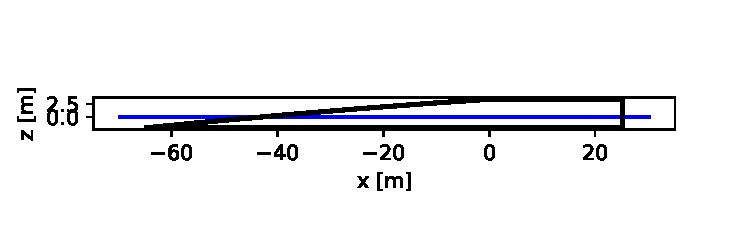
\includegraphics[width=\textwidth]{figures/ComFLOW/Breakwater Geometries/Design Iteration 1 captive/general/breakwater_geometry24.pdf}
        \caption[]%
        {{\small}configuration 24}    
        \label{fig: It1 Configuration 16}
    \end{subfigure}
    \hfill
    \begin{subfigure}[b]{0.49\textwidth}  
        \centering 
        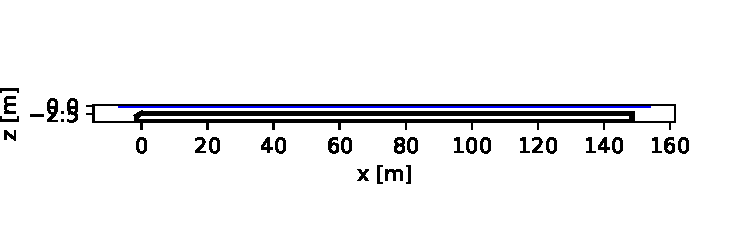
\includegraphics[width=\textwidth]{figures/ComFLOW/Breakwater Geometries/Design Iteration 1 captive/general/breakwater_geometry45.pdf}
        \caption[]%
        {{\small}configuration 45}    
        \label{fig: It1 Configuration 24}
    \end{subfigure}
    \vskip\baselineskip
    \begin{subfigure}[b]{0.49\textwidth}   
        \centering 
        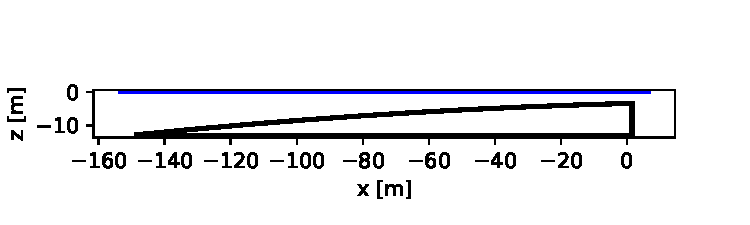
\includegraphics[width=\textwidth]{figures/ComFLOW/Breakwater Geometries/Design Iteration 1 captive/general/breakwater_geometry16.pdf}
        \caption[]%
        {{\small}configuration 16}    
        \label{fig: It1 Configuration 32}
    \end{subfigure}
    \hfill
    \begin{subfigure}[b]{0.49\textwidth}   
        \centering 
        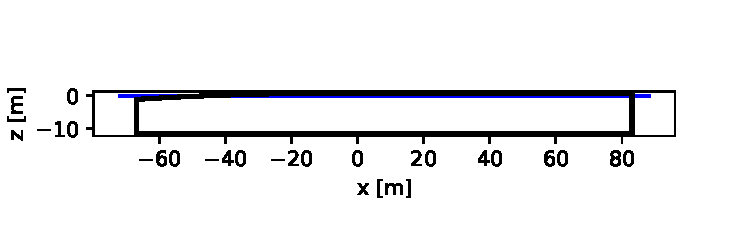
\includegraphics[width=\textwidth]{figures/ComFLOW/Breakwater Geometries/Design Iteration 1 captive/general/breakwater_geometry37.pdf}
        \caption[]%
        {{\small}configuration 37}    
        \label{fig: It1 Configuration 37}
    \end{subfigure}
    \hfill
    \begin{subfigure}[b]{0.49\textwidth}   
        \centering 
        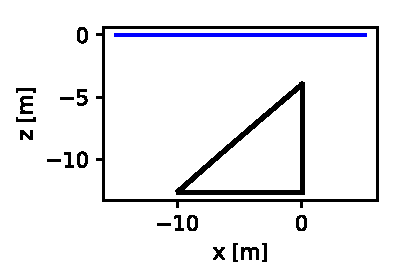
\includegraphics[width=0.5\textwidth]{figures/ComFLOW/Breakwater Geometries/Design Iteration 1 captive/general/breakwater_geometry32.pdf}
        \caption[]%
        {{\small}configuration 32}    
        \label{fig: It1 Configuration 40}
    \end{subfigure}
        \hfill
    \begin{subfigure}[b]{0.49\textwidth}   
        \centering 
        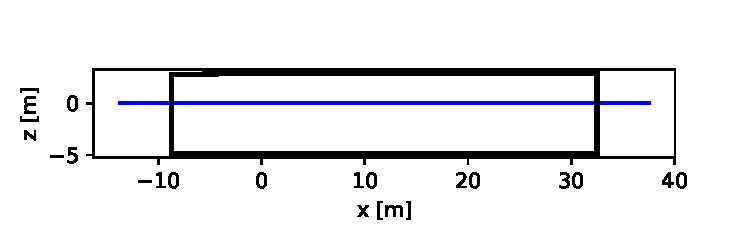
\includegraphics[width=\textwidth]{figures/ComFLOW/Breakwater Geometries/Design Iteration 1 captive/general/breakwater_geometry40.pdf}
        \caption[]%
        {{\small}configuration 40}    
        \label{fig: It1 Configuration 45}
    \end{subfigure}
    
    \caption{Six different configurations of the first design iteration}
    \label{fig:Configurations 1to6 DI1 captive}
\end{figure}


The performance of each breakwater is quantified after all configurations of the design space were simulated in ComFLOW by studying the influence of the magnitude of the factors (T, W, front\_fraction, top\_fraction and WL) on the responses (mean wave drift force and wave transmission). The mean wave drift force is nondimensionalised by dividing it through the mean wave load on a wall, this quantity is called $F_{d,norm}$ (equation \ref{eq: handling Fdnorm}). Wave transmission is studied through the wave transmission coefficient $K_t$, which is the ratio between the transmitted wave height and the incident wave height. Note again that the factor WL, which defines the position z of the breakwater, shifts the waterline with regard to the origin of the body-fixed coordinate system (see Figure \ref{fig: parametrisation breakwater}), which is on top of the breakwater behind the sloping beach (see Figure \ref{fig: parametrisation breakwater}). For example, with WL = 1 the top of the breakwater is one metre below the waterline and WL = -1 means one metre of the breakwater is above the waterline.




\subsection{Performance breakwaters}
\label{sec: DI1 captive H3 performance bw}

% -performance breakwaters mapped to plot their mean wave drift force wrt wave transmission
% -configuration 5 probably a unreasonably low mean wave drift force. 
% -best performing at wave attenuation are large boxes underneath close to waterline, it is expected. Expected by literature (linear wave theory)
% -best at having a low mean wave drift force are large wedge-type structures. Expected by literature--> dissipation leads to lowering mean wave drift force

The performance of the 94 breakwaters of the design space of this first design iteration is mapped in Figure \ref{fig: Fd vs. Kt DI1 H3 captive}, where the normalised mean wave drift force (F$_{d,norm}$) is plotted against the wave transmission coefficient (K$_t$ = H$_t$/H$_i$). Figure \ref{fig: Fd vs. Kt DI1 H3 captive pareto} is zoomed in on the Pareto front (the set of most efficient solutions in a multi-objective optimisation) and the shape of these best performing breakwaters is shown in Figure \ref{fig: pareto front bw DI1 H3 captive}. The breakwaters that perform best in attenuating wave energy on this Pareto front are very large box-type structures (high depth and width) and are placed around the waterline with their top. Those on the Pareto front best at minimising the mean wave drift force are structures placed further beneath the water surface and possess a sloping beach which induces the incoming waves to break and thereby dissipate wave energy.  


Note that configuration 5 is not included in the Pareto front, because it gave results from which it is not sure whether this is an accurate representation of reality. The average water level of the simulation of this breakwater is shown in Figure \ref{fig: average wl configuration 5}, from which can be seen that a large set-down of the water level is present in front of the structure. This is caused by a downwards fluid flow, shown in Figure \ref{fig: fluid flow configuration 5}. Over time can be seen that the waves break on the breakwaters surface, after which the fluid particles on top flow back (into the direction of negative x) and once the fluid particles flow over the edge they are sucked to the bottom of the domain. This causes a low pressure region and this might be the reason the geometry has experiences a very low mean wave drift force over time. 

\begin{figure}[h]
    \centering
    \begin{subfigure}[b]{0.49\textwidth}
        \centering
        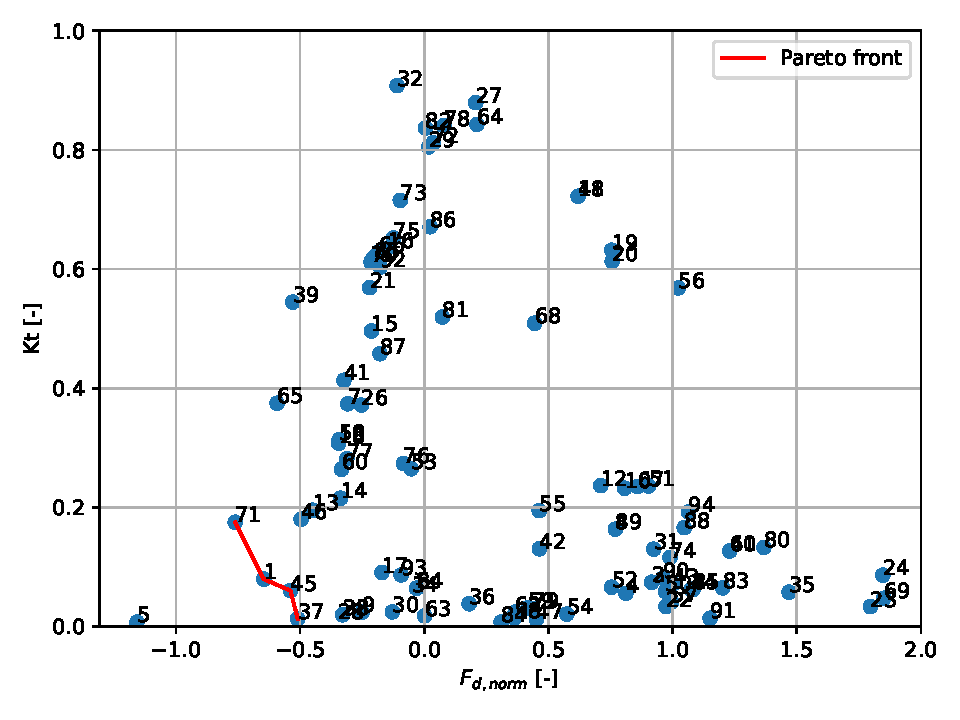
\includegraphics[width=\linewidth]{figures/ComFLOW/Results DI1/Fd_norm_VS_Kt_normal.pdf}
        \caption[]%
        {{\small All breakwaters}}    
        \label{fig: Fd vs. Kt DI1 H3 captive normal}
    \end{subfigure}
    \hfill
    \begin{subfigure}[b]{0.49\textwidth}  
        \centering 
        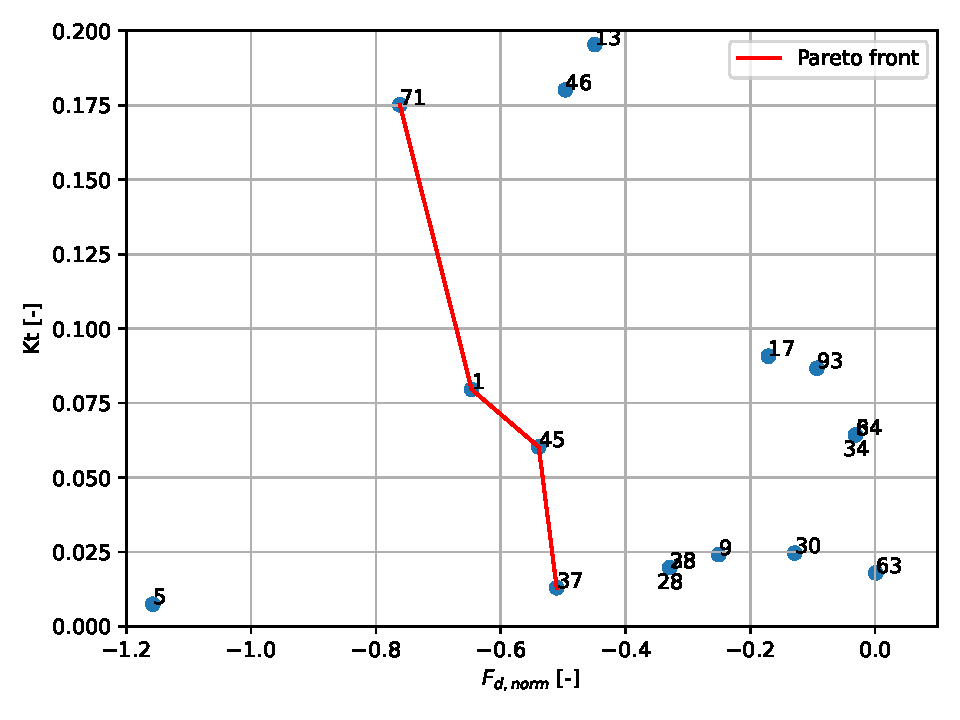
\includegraphics[width=\linewidth]{figures/ComFLOW/Results DI1/Fd_norm_VS_Kt_Pareto.pdf}
        \caption[]%
        {{\small Pareto front}}    
        \label{fig: Fd vs. Kt DI1 H3 captive pareto}
    \end{subfigure}
    
    \caption{Mean wave drift force Vs. Wave transmission}
    \label{fig: Fd vs. Kt DI1 H3 captive}
\end{figure}




\begin{figure}[h]
    \centering
    \begin{subfigure}[b]{0.49\textwidth}
        \centering
        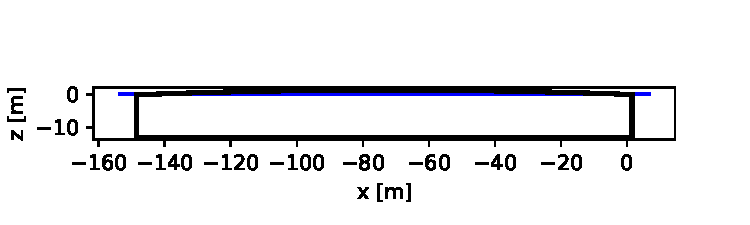
\includegraphics[width=\linewidth]{figures/ComFLOW/Breakwater Geometries/Design Iteration 1 captive/general/breakwater_geometry5.pdf}
        \caption[]%
        {{\small Configuration 5}}    
        \label{}
    \end{subfigure}
    \hfill
    \begin{subfigure}[b]{0.49\textwidth}  
        \centering 
        \includegraphics[width=\linewidth]{figures/ComFLOW/Breakwater Geometries/Design Iteration 1 captive/general/breakwater_geometry37.pdf}
        \caption[]%
        {{\small Configuration 37}}    
        \label{}
    \end{subfigure}
    
    \centering
    \begin{subfigure}[b]{0.49\textwidth}
        \centering
        \includegraphics[width=\linewidth]{figures/ComFLOW/Breakwater Geometries/Design Iteration 1 captive/general/breakwater_geometry45.pdf}
        \caption[]%
        {{\small Configuration 45}}    
        \label{}
    \end{subfigure}
    \hfill
    \begin{subfigure}[b]{0.49\textwidth}  
        \centering 
        \includegraphics[width=\linewidth]{figures/ComFLOW/Breakwater Geometries/Design Iteration 1 captive/general/breakwater_geometry1.pdf}
        \caption[]%
        {{\small Configuration 1}}    
        \label{}
    \end{subfigure}
    
    \centering
    \begin{subfigure}[b]{0.49\textwidth}
        \centering
        \includegraphics[width=\linewidth]{figures/ComFLOW/Breakwater Geometries/Design Iteration 1 captive/general/breakwater_geometry71.pdf}
        \caption[]%
        {{\small Configuration 71}}    
        \label{}
    \end{subfigure}
    
    \caption{Wave breakers on Pareto front}
    \label{fig: pareto front bw DI1 H3 captive}
\end{figure}



\begin{figure}[h]
    \centering
    \begin{subfigure}[b]{0.49\textwidth}
        \centering
        \includegraphics[width=\linewidth]{figures/ComFLOW/Results average wl/configuration5.pdf}
        \caption[]%
        {{\small Average water level}}    
        \label{fig: average wl configuration 5}
    \end{subfigure}
    \hfill
    \begin{subfigure}[b]{0.49\textwidth}  
        \centering 
        \includegraphics[width=\linewidth]{figures/ComFLOW/Results DI1/config_5_run_23.png}
        \caption[]%
        {{\small Downwards fluid flow in front of breakwater}}    
        \label{fig: fluid flow configuration 5}
    \end{subfigure}
    
    \caption{Visualisation of low pressure field in front of configuration 5}
    \label{fig: configuration 5 low pressure field }
\end{figure}





\subsection{Correlation}
\label{sec: DI1 captive H3 correlation}


Figure \ref{fig: correlation DI1 captive} shows the correlation between all the factors and responses. Where red means a positive correlation and blue a negative. So, from this Figure can be concluded a large floater width $W$ leads to a small transmission coefficient $K_t$ and a deeply submerged breakwater (high $WL$) leads to a high wave transmission but low mean wave drift force. Figures \ref{fig: perturbation R1 DI1 captive} and \ref{fig: perturbation R2 DI1 captive} show the trend of the a change in factors (A to F) on respectively the mean wave drift force (Fd\_norm) and the transmitted wave height (Kt$^2$).\\
\\
Figures \ref{fig: perturbation R1 DI1 captive} shows that the mean wave drift force is negatively correlated with the z position of the breakwater (factor F), with its minimum around 1.5 metres below the waterline. This correlation is present for the largest part of the spectrum, but there is a positive correlation at the boundaries (i.e. its maximum and minimum lie within the design space boundaries). The same trend is observed in Figure \ref{fig: Fd_norm_VS_top_bw_with_Kt DI1 captive H3}, where the mean wave drift force of the breakwaters of the design space is plotted against the z position of the body-fixed origin w.r.t. the waterline. From this Figure can be seen that most submerged breakwaters experienced a negative mean wave drift force, while some of them also have good wave attenuation performance. \\
Also, the correlation between factor F and the wave transmission  coefficient (figure \ref{fig: perturbation R2 DI1 captive}) shows that breakwaters where the origin of the body-fixed coordinate system is placed between 0 and 2 metres above the water level perform best, at attenuating wave energy. When the breakwater would be placed higher or lower than this optimum, it would perform less (higher $K_t$), with a stronger correlation when factor F rises (i.e. while the breakwater will be positioned deeper, its wave attenuating performance decreases significantly). Also, in this Figure could be observed the negative correlation between the floater width (factor B) and the wave transmission is stronger for small floater widths.\\
Furthermore, the wave transmission $K_t$ has a negative correlation with the mean wave drift force $F_{d,norm}$. In other words, when a large mean wave drift force occurs a small transmission coefficient is present, on average. 



\begin{figure}[h]
    \centering
    \begin{subfigure}[b]{0.30\textwidth}  
        \centering 
        \includegraphics[width=\linewidth]{figures/ComFLOW/Results DI1/correlation.png}
        \caption[]%
        {{\small Correlation between factors and responses}}    
        \label{fig: correlation DI1 captive}
    \end{subfigure}
    \hfill
    \begin{subfigure}[b]{0.49\textwidth}
        \centering
        \includegraphics[width=\linewidth]{figures/ComFLOW/Results DI1/Fd_norm_VS_top_bw_with_Kt.pdf}
        \caption[]%
        {{\small Mean wave drift force to z-positioning breakwaters}}    
        \label{fig: Fd_norm_VS_top_bw_with_Kt DI1 captive H3}
    \end{subfigure}

    \caption{}
    \label{fig: }
\end{figure}    
    
\begin{figure}[h]
    \centering
    \begin{subfigure}[b]{0.49\textwidth}
        \centering
        \includegraphics[width=\linewidth]{figures/ComFLOW/Results DI1/perturbation R1.pdf}
        \caption[]%
        {{\small Perturbation Response 1: Mean wave drift force}}    
        \label{fig: perturbation R1 DI1 captive}
    \end{subfigure}
    \hfill
    \begin{subfigure}[b]{0.49\textwidth}  
        \centering 
        \includegraphics[width=\linewidth]{figures/ComFLOW/Results DI1/perturbation R2.pdf}
        \caption[]%
        {{\small Perturbation Response 2: Wave transmission coefficient}}    
        \label{fig: perturbation R2 DI1 captive}
    \end{subfigure}


    \caption{}
    \label{fig: }
\end{figure}





\subsection{Response Surfaces}
\label{sec: DI1 captive H3 response surfaces}

Unfortunately we are limited to visualise our results in three dimensions. Where one response, either the normalised mean wave drift force or the transmission coefficient, is put at one axis and two input parametres on the others. In each of the following plots, the remaining four parametres are kept constant at value where the plot shows interesting results. Evidently, the response surface looks different when other values for these parametres are chosen. Therefore, in this section, the two extreme shapes are studied. When the factors \textit{top\_fraction} and \textit{front\_fraction} are 0.99, the breakwater is a box-type structure and when these factors both are 0.01, it is a wedge with a large inclined beach.  \\
Note that in this section the response surfaces and the way to implement them is extensively discussed, this is not done in the remaining sections. \\
\\
Figure \ref{fig: Fd_W_T_box DI1 H3 captive} shows the dependency of the width and depth of the a wedge-type breakwater on the mean wave drift force. The correlation between the floater width $W$ and the response is minor, but the structures depth $T$ and the mean wave drift force show a strong, negative correlation (i.e. a large $T$ leads to a small $\Bar{F_d}$ for wedge-type breakwaters). Figure \ref{fig: Fd_W_T_box DI1 H3 captive} shows that for a box-type breakwater, the correlation between the factors A and B (floater width $W$ and depth $T$) and the mean wave drift force is minor.\\
The dependency of the factors B and F (the floater width $W$ and z-positioning of the breakwater $WL$) on the mean wave drift force is shown in Figure \ref{fig: Fd_W_WL_box DI1 H3 captive} and \ref{fig: Fd_W_WL_box DI1 H3 captive}. Again, the dependency on the floater width is minor, but the z-positioning of the floater is strongly correlated with the mean wave drift force, with its minimum around 3 metres below the waterline.\\
Figure \ref{fig: Fd_W_WL_wedge DI1 H3 captive} shows two minima when factor A and F (breakwater's depth $T$ and its z-position $WL$). Relatively shallow wedge-type breakwaters ($T$=2.5) experience a low mean wave drift force when they are placed around 3 metres below the waterline and wedge-type structures with a large depth (11<$T$<13) perform best around the waterline. Box-type structures do not depend strongly on their depth, shows Figure \ref{fig: Fd_W_WL_box DI1 H3 captive}.





\begin{figure}[h]
    \centering
    \begin{subfigure}[b]{0.49\textwidth}
        \centering
        \includegraphics[width=\textwidth]{figures/ComFLOW/Results DI1/Fd_W_T_box_png.png}
        \caption[]%
        {{\small $W$ and $T$ w.r.t. $F_{d,norm}$ box-type}}    
        \label{fig: Fd_W_T_box DI1 H3 captive}
    \end{subfigure}
    \hfill
    \begin{subfigure}[b]{0.49\textwidth}  
        \centering 
        \includegraphics[width=\textwidth]{figures/ComFLOW/Results DI1/Fd_W_T_wedge_png.png}
        \caption[]%
        {{\small $W$ and $T$ w.r.t. $F_{d,norm}$ wedge-type}}    
        \label{fig: Fd_W_T_wedge DI1 H3 captive}
    \end{subfigure}
    \vskip\baselineskip
    \begin{subfigure}[b]{0.49\textwidth}   
        \centering 
        \includegraphics[width=\textwidth]{figures/ComFLOW/Results DI1/Fd_W_WL_box_png.png}
        \caption[]%
        {{\small $W$ and $WL$ w.r.t. $F_{d,norm}$ box-type}}    
        \label{fig: Fd_W_WL_box DI1 H3 captive}
    \end{subfigure}
    \hfill
    \begin{subfigure}[b]{0.49\textwidth}   
        \centering 
        \includegraphics[width=\textwidth]{figures/ComFLOW/Results DI1/Fd_W_WL_wedge_png.png}
        \caption[]%
        {{\small $W$ and $WL$ w.r.t. $F_{d,norm}$ wedge-type}}    
        \label{fig: Fd_W_WL_wedge DI1 H3 captive}
    \end{subfigure}

    \vskip\baselineskip
    \begin{subfigure}[b]{0.49\textwidth}   
        \centering 
        \includegraphics[width=\textwidth]{figures/ComFLOW/Results DI1/FD_T_WL_box_png.png}
        \caption[]%
        {{\small $T$ and $WL$ w.r.t. $F_{d,norm}$ box-type}}    
        \label{fig: Fd_T_WL_box DI1 H3 captive}
    \end{subfigure}
    \hfill
    \begin{subfigure}[b]{0.49\textwidth}   
        \centering 
        \includegraphics[width=\textwidth]{figures/ComFLOW/Results DI1/FD_T_WL_wedge_png.png}
        \caption[]%
        {{\small $T$ and $WL$ w.r.t. $F_{d,norm}$ wedge-type}}    
        \label{fig: Fd_T_WL_wedge DI1 H3 captive}
    \end{subfigure}


    \caption{Dependency different factors on $F_{d,norm}$}
    \label{fig: Dependency different parametres on Fd  DI1 H3 captive}
\end{figure}



Figure \ref{fig: Dependency different parametres on Kt  DI1 H3 captive} shows how the transmission coefficient depends on the width $W$, the position of the waterline $WL$ and the depth $T$. Figure \ref{fig: Kt_W_T_box DI1 H3 captive} and \ref{fig: Kt_W_T_wedge DI1 H3 captive} visualise how $K_t$ changes while $W$ and $T$ change. A strong dependence on the width of the floater is observed for both a box-type structure and a wedge-type structure, where $K_t$ decreases while $W$ increases. At small floater widths, the dependence on the structures depth is minor, but this dependency increases while the width increases, where a large T leads to a low transmission coefficient. \acrfull{doe} expects some configurations will even have a negative transmission coefficient, but this is, of course, physically impossible. \\
Figure \ref{fig: Kt_W_WL_box DI1 H3 captive} and \ref{fig: Kt_W_WL_wedge DI1 H3 captive} shows that the optimal position of the waterline is around the top of the breakwater ($WL$=0). Also, it shows that for breakwaters that are placed very deep under water, the floater width has a minor effect on $K_t$. In addition, wedge-type structures need to be higher to have the same wave transmission performance as box-type structures.\\
In \ref{fig: Kt_T_WL_box DI1 H3 captive} and \ref{fig: Kt_W_TL_wedge DI1 H3 captive} the dependence of the floater depth $T$ and position of the waterline $WL$ on the wave transmission can be observed. The correlation between the depth of the structure $T$ and the response is strong for box- and wedge-type breakwaters above the waterline ($WL$ < 0), but this correlation decreases as the breakwater is placed deeper. Box-type breakwaters find their minimal wave transmission coefficient when their body-fixed origin (their top) is placed around the waterline, and wedge-type breakwaters need to be placed above the waterline to attenuate the most wave energy. 

\begin{figure}[h]
    \centering
    \begin{subfigure}[b]{0.49\textwidth}
        \centering
        \includegraphics[width=\textwidth]{figures/ComFLOW/Results DI1/Kt_W_T_box_png.png}
        \caption[]%
        {{\small $W$ and $T$ w.r.t. $K_{t}$ box-type}}    
        \label{fig: Kt_W_T_box DI1 H3 captive}
    \end{subfigure}
    \hfill
    \begin{subfigure}[b]{0.49\textwidth}  
        \centering 
        \includegraphics[width=\textwidth]{figures/ComFLOW/Results DI1/Kt_W_T_wedge_png.png}
        \caption[]%
        {{\small $W$ and $T$ w.r.t. $K_{t}$ wedge-type}}    
        \label{fig: Kt_W_T_wedge DI1 H3 captive}
    \end{subfigure}
    \vskip\baselineskip
    \begin{subfigure}[b]{0.49\textwidth}   
        \centering 
        \includegraphics[width=\textwidth]{figures/ComFLOW/Results DI1/Kt_W_WL_box_png.png}
        \caption[]%
        {{\small $W$ and $WL$ w.r.t. $K_{t}$ box-type}}    
        \label{fig: Kt_W_WL_box DI1 H3 captive}
    \end{subfigure}
    \hfill
    \begin{subfigure}[b]{0.49\textwidth}   
        \centering 
        \includegraphics[width=\textwidth]{figures/ComFLOW/Results DI1/Kt_W_WL_wedge_png.png}
        \caption[]%
        {{\small $W$ and $WL$ w.r.t. $K_{t}$ wedge-type}}    
        \label{fig: Kt_W_WL_wedge DI1 H3 captive}
    \end{subfigure}
    
    \vskip\baselineskip
    \begin{subfigure}[b]{0.49\textwidth}   
        \centering 
        \includegraphics[width=\textwidth]{figures/ComFLOW/Results DI1/Kt_T_WL_box_png.png}
        \caption[]%
        {{\small $T$ and $WL$ w.r.t. $K_{t}$ box-type}}    
        \label{fig: Kt_T_WL_box DI1 H3 captive}
    \end{subfigure}
    \hfill
    \begin{subfigure}[b]{0.49\textwidth}   
        \centering 
        \includegraphics[width=\textwidth]{figures/ComFLOW/Results DI1/Kt_T_WL_wedge_png.png}
        \caption[]%
        {{\small $T$ and $WL$ w.r.t. $K_{t}$ wedge-type}}    
        \label{fig: Kt_W_TL_wedge DI1 H3 captive}
    \end{subfigure}

    \caption{Dependency different parametres on $K_t^2$}
    \label{fig: Dependency different parametres on Kt  DI1 H3 captive}
\end{figure}



\subsection{Design Optima}
\label{sec: DI1 captive H3 design optima}

Based on the constructed response surfaces, design optima are made and announced in this section. First, based on a minimal mean wave drift force. Then, based on a minimal wave transmission coefficient, and lastly optima are given where both responses are minimised. 


\subsubsection{Based on minimal mean wave drift force}
The ten breakwaters which perform best in minimizing the mean wave drift force are presented in Table \ref{tab: params design iteration 1 captive br 1to10 min drift force H3}, on the order of desirability (i.e. Design Expert expects configuration 1 to perform best). The first two configurations are visualised in Figures \ref{fig: opt breakwater 1 FD DI1 H3 captive} and \ref{fig: opt breakwater 2 FD DI1 H3 captive}. Two variants were given. One box-type structure that converged to the smallest depth $T$, and has a width $W$ of 63 metres and is placed 1,5 metres below the waterline. The other has a larger depth of 11.6 metres, maximum width of 150 metres, has a sloping beach at its wave-ward side and is placed with its top 1.3 metres below the water surface. 

\begin{table}[h]
\centering
\scalebox{0.65}{
\begin{tabular}{@{}ccccccccccc@{}}
\toprule
configuration & T        & W        & front\_fraction & top\_fraction & radius   & WL & $F_{d,norm,DoE}$ & $K_{t,DoE}^2$  & $F_{d,norm,ComFLOW}$  & $K_{t,ComFLOW}^2$      \\ \midrule
1  & 2.51  & 63.69  & 0.05 & 0.99 & 500.33  & 1.45 & -0.83 & 0.00 & -0.52 & 0.04 \\
2  & 2.50  & 69.97  & 0.04 & 0.99 & 501.98  & 1.46 & -0.83 & 0.00  & -0.56 & 0.03\\
3  & 11.67 & 149.99 & 0.79 & 0.26 & 1853.19 & 1.33 & -0.81 & -0.02 & -0.46 & 0.02\\
4  & 11.66 & 150.00 & 0.84 & 0.27 & 1847.63 & 1.34 & -0.81 & -0.03 \\
5  & 12.11 & 150.00 & 0.68 & 0.21 & 1810.66 & 0.87 & -0.81 & 0.00  \\
6  & 11.59 & 150.00 & 0.90 & 0.29 & 1850.82 & 1.41 & -0.81 & -0.04 \\
7  & 11.61 & 148.70 & 0.93 & 0.25 & 1850.26 & 1.39 & -0.81 & -0.05 \\
8  & 11.62 & 150.00 & 0.63 & 0.24 & 1664.65 & 1.38 & -0.81 & 0.00  \\
9  & 11.56 & 150.00 & 0.82 & 0.19 & 1938.78 & 1.44 & -0.80 & -0.02 \\
10 & 11.30 & 150.00 & 0.95 & 0.35 & 1926.44 & 1.70 & -0.80 & -0.04\\ \bottomrule
\end{tabular}
}
\caption{Parameters optimal breakwaters based on minimal mean wave drift force}
\label{tab: params design iteration 1 captive br 1to10 min drift force H3}
\end{table}


\begin{figure}[h]
    \centering
    \begin{subfigure}[b]{0.49\textwidth}
        \centering
        \includegraphics[width=\textwidth]{figures/ComFLOW/Breakwater Geometries/Design Iteration 1 captive/top6 low Fd/breakwater_geometry1.pdf}
        \caption[]%
        {{\small}}    
        \label{fig: opt breakwater 1 FD DI1 H3 captive}
    \end{subfigure}
    \hfill
    \begin{subfigure}[b]{0.49\textwidth}  
        \centering 
        \includegraphics[width=\textwidth]{figures/ComFLOW/Breakwater Geometries/Design Iteration 1 captive/top6 low Fd/breakwater_geometry3.pdf}
        \caption[]%
        {{\small}}    
        \label{fig: opt breakwater 2 FD DI1 H3 captive}
    \end{subfigure}
    
    \caption{The two most optimal breakwaters based on the mean wave drift force}
    \label{fig: two most optimal breakwaters FD DI1 H3 captive}
\end{figure}


\subsubsection{Based on minimal transmission coefficient}
The breakwaters shown in Table Table \ref{tab: params design iteration 1 captive br 1to10 min transmission coefficient} perform best in attenuating waves, according to the predictions of Design Expert.
\begin{table}[h]
\centering
\scalebox{0.65}{
\begin{tabular}{@{}ccccccccccc@{}}
\toprule
configuration & T        & W        & front\_fraction & top\_fraction & radius   & WL & $F_{d,norm,DoE}$ & $K_{t,DoE}^2$  & $F_{d,norm,ComFLOW}$  & $K_{t,ComFLOW}^2$      \\ \midrule
1  & 7.632  & 88.726  & 0.865 & 0.837 & 1816.704 & -0.739 & 0.468  & -0.032 \\
2  & 10.946 & 100.297 & 0.943 & 0.178 & 1833.333 & -1.966 & 0.370  & -0.023 \\
3  & 12.673 & 36.254  & 0.926 & 0.984 & 1470.102 & 0.179  & 0.127  & -0.011 \\
4  & 12.136 & 58.088  & 0.108 & 0.990 & 950.000  & -0.864 & 0.626  & -0.040 \\
5  & 10.170 & 32.930  & 0.728 & 0.505 & 1543.715 & -2.296 & 0.701  & -0.062 \\
6  & 3.046  & 58.675  & 0.038 & 0.445 & 1884.668 & -1.136 & 1.041  & -0.012 \\
7  & 12.738 & 150.000 & 0.133 & 0.059 & 500.000  & 0.000  & -0.044 & -0.011 \\
8  & 6.900  & 117.100 & 0.191 & 0.618 & 1250.000 & -6.100 & 0.835  & -0.021 \\
9  & 9.753  & 119.900 & 0.010 & 0.010 & 949.795  & -3.247 & 0.943  & -0.017 \\
10 & 7.497  & 147.582 & 0.797 & 0.652 & 1891.990 & 1.321  & -0.222 & -0.023 \\ \bottomrule
\end{tabular}
}
\caption{Parameters optimal breakwaters based on minimal transmission coefficient}
\label{tab: params design iteration 1 captive br 1to10 min transmission coefficient}
\end{table}




% \subsection{Discussion}

% -negative, exponential correlation between W and Kt, corresponds with macagno and validation chapter\\
% -positive correlation between WL and mean wvae drift force for middle part of spectrum boundaries of DI1\\
% -the breakwaters where waves are breaking by spilling, seem to have a lower mean wave drift force on average. \\



% \subsection{Conclusions}


\section{Design Iteration 2}
\label{sec: design iteration 2 captive}
The first design iteration is suitable to map the response surfaces over a wide spectrum of input factors and thus determine the rough location of the optima. But due to the wide variety of the data points, the reliability of the output optima is limited. However, this can be increased by doing a second design iteration, where a new design space is made with a narrower design spectrum, where the parameter boundaries are less spread and lie around the optima.

\subsection{Approach}
Based on the results of the first design iteration, the boundaries for the second design iteration are established and shown in Table \ref{tab: boundaries DI2 captive}. The complete design space, including results, is shown in Table \ref{tab: params design iteration 2 captive setup} Appendix \ref{app: parameters configurationss}.

\begin{table}[h]
\centering
\scalebox{0.65}{
\begin{tabular}{@{}ccccc@{}}
\toprule
Factor & Name        & Units        & Minimum & Maximum       \\ \midrule
A & T               & m & 9.50   & 12.50   \\
B & W               & m & 120.00  & 150.00   \\
C & front\_fraction & - & 0.010 & 0.99  \\
D & top\_fraction   & - & 0.010 & 0.99  \\
E & radius          & m & 1500.00 & 2000.00 \\
F & WL              & m & 0.50  & 2.50     \\ \bottomrule
\end{tabular}
}
\caption{Boundaries Design Space Captive Design Iteration 2}
\label{tab: boundaries DI2 captive}
\end{table}

\subsection{Performance breakwaters}
\label{sec: DI1 captive H3 performance bw}

The performance of the breakwater in terms of minimising the mean wave drift force and maximising wave attenuation is shown in Figure \ref{fig: Fd vs. Kt DI2 H3 captive}, from which it can be seen that now more breakwaters are indeed performing better in both phenomena, compared to the first design iteration. The Pareto front obviously consists of more breakwaters. Some of them have a geometry shown in Figure \ref{fig: pareto front bw DI2 H3 captive}. Again, large box-type structures around the waterline are best at attenuating wave energy, and those containing a sloping beach on their wave-ward side are good at minimising the mean wave drift force. 


\begin{figure}[h]
    \centering
    \begin{subfigure}[b]{0.49\textwidth}
        \centering
        \includegraphics[width=\linewidth]{figures/ComFLOW/Results DI2/Fd_norm_VS_Kt_normal.pdf}
        \caption[]%
        {{\small All breakwaters}}    
        \label{fig: Fd vs. Kt DI2 H3 captive normal}
    \end{subfigure}
    \hfill
    \begin{subfigure}[b]{0.49\textwidth}  
        \centering 
        \includegraphics[width=\linewidth]{figures/ComFLOW/Results DI2/Fd_norm_VS_Kt_Pareto.pdf}
        \caption[]%
        {{\small Pareto front}}    
        \label{fig: Fd vs. Kt DI2 H3 captive pareto}
    \end{subfigure}
    
    \caption{Mean wave drift force vs. Wave transmission}
    \label{fig: Fd vs. Kt DI2 H3 captive}
\end{figure}



\begin{figure}[h]
    \centering
    \begin{subfigure}[b]{0.49\textwidth}
        \centering
        \includegraphics[width=\linewidth]{figures/ComFLOW/Breakwater Geometries/Design Iteration 2 captive/breakwater_geometry94.pdf}
        \caption[]%
        {{\small }}    
        \label{}
    \end{subfigure}
    \hfill
    \begin{subfigure}[b]{0.49\textwidth}  
        \centering 
        \includegraphics[width=\linewidth]{figures/ComFLOW/Breakwater Geometries/Design Iteration 2 captive/breakwater_geometry80.pdf}    
        {{\small }}    
        \label{}
    \end{subfigure}
    
    \centering
    \begin{subfigure}[b]{0.49\textwidth}
        \centering
        \includegraphics[width=\linewidth]{figures/ComFLOW/Breakwater Geometries/Design Iteration 2 captive/breakwater_geometry64.pdf}    
        \caption[]%
        {{\small }}    
        \label{}
    \end{subfigure}
    \hfill
    \begin{subfigure}[b]{0.49\textwidth}  
        \centering 
        \includegraphics[width=\linewidth]{figures/ComFLOW/Breakwater Geometries/Design Iteration 2 captive/breakwater_geometry51.pdf}    
        \caption[]%
        {{\small }}    
        \label{}
    \end{subfigure}
    
    \centering
    \begin{subfigure}[b]{0.49\textwidth}
        \centering
        \includegraphics[width=\linewidth]{figures/ComFLOW/Breakwater Geometries/Design Iteration 2 captive/breakwater_geometry41.pdf}    
        \caption[]%
        {{\small }}    
        \label{}
    \end{subfigure}
    \hfill
    \begin{subfigure}[b]{0.49\textwidth}  
        \centering 
        \includegraphics[width=\linewidth]{figures/ComFLOW/Breakwater Geometries/Design Iteration 2 captive/breakwater_geometry25.pdf}    
        \caption[]%
        {{\small }}    
        \label{}
    \end{subfigure}
    
    \caption{Wave breakers on Pareto front}
    \label{fig: pareto front bw DI2 H3 captive}
\end{figure}





\subsection{Design Optima}
Based on the data found by ComFLOW, the response surfaces were plotted from which the design optima are found and presented in this section. 


\subsubsection{Based on minimal mean wave drift force}
Again, the first six optima based on a minimal mean wave drift force converged to the lowest value of $T$. Therefore, the structure is placed slightly closer to the waterline, which is consistent with the response surface of Figure \ref{fig: Fd_T_WL_wedge DI1 H3 captive}. In addition, these optima converged to the lowest width $W$. All the top fractions of configurations 1 to 6 are 0.99, so they are box-type structures. 
The last four optima are larger structures, placed closer to the water surface and possess a sloping beach. Configurations 1 and 7 experienced the same mean wave drift force, but Configuration 1 has better wave attenuation performances. 


\begin{table}[h]
\centering
\scalebox{0.65}{
\begin{tabular}{@{}ccccccccccc@{}}
\toprule
configuration & T        & W        & front\_fraction & top\_fraction & radius   & WL & $F_{d,norm,DoE}$ & $K_{t,DoE}^2$  & $F_{d,norm,ComFLOW}$  & $K_{t,ComFLOW}^2$      \\ \midrule
1  & 9.50  & 120.00 & 0.59 & 0.99 & 1500.00 & 2.16 & -0.96 & 0.009  & -0.51 & 0.043\\
2  & 9.52  & 120.00 & 0.58 & 0.99 & 1500.00 & 2.17 & -0.95 & 0.009  \\
3  & 9.51  & 121.03 & 0.58 & 0.99 & 1500.04 & 2.14 & -0.95 & 0.008  \\
4  & 9.50  & 126.18 & 0.58 & 0.99 & 1500.00 & 2.06 & -0.94 & 0.005  \\
5  & 9.50  & 120.00 & 0.52 & 0.97 & 1500.00 & 2.24 & -0.94 & 0.010  \\
6  & 9.50  & 122.12 & 0.47 & 0.99 & 1502.39 & 1.92 & -0.94 & 0.005  \\
7  & 12.11 & 150.00 & 0.010 & 0.66 & 1519.49 & 0.89 & -0.94 & -0.002 &-0.51 & 0.080 \\
8  & 12.21 & 150.00 & 0.010 & 0.64 & 1542.35 & 0.79 & -0.93 & -0.002 \\
9  & 12.08 & 149.97 & 0.010 & 0.68 & 1543.32 & 0.92 & -0.93 & -0.001 \\
10 & 12.18 & 150.00 & 0.010 & 0.62 & 1508.26 & 0.82 & -0.93 & -0.002 \\ \bottomrule


\end{tabular}
}
\caption{Parameters optimal breakwaters based on minimal mean wave drift force}
\label{tab: most optimal breakwaters DI2 Fd}
\end{table}


\begin{figure}[h]
    \centering
    \begin{subfigure}[b]{0.475\textwidth}
        \centering
        \includegraphics[width=\textwidth]{figures/ComFLOW/Breakwater Geometries/Design Iteration 2 captive/breakwater_geometry1_Fd.pdf}
        \caption[]%
        {{\small}}    
        \label{fig: opt breakwater 1 DI2}
    \end{subfigure}
    \hfill
    \begin{subfigure}[b]{0.475\textwidth}
        \centering
        \includegraphics[width=\textwidth]{figures/ComFLOW/Breakwater Geometries/Design Iteration 2 captive/breakwater_geometry2_Fd.pdf}
        \caption[]%
        {{\small}}    
        \label{fig: opt breakwater 1 DI2}
    \end{subfigure}
    \caption{The most optimal breakwaters based on mean wave drift force}
    \label{fig:  most optimal breakwaters DI2}
\end{figure}









\subsubsection{Based on minimal transmission coefficient}
Most of the design optima converged to a depth $T$ within the parameter limits. Interesting is that for wave transmission performance, the breakwaters did not converge to the largest width $W$. The biggest difference in comparison with the first six optima based on a minimal mean wave drift force (previous section) is that the breakwaters are placed closer to the waterline and a large sloping beach is present. The optima are similar to optima 7 to 10 of previous section. All optima found also have a negative mean wave drift force. 



\begin{table}[h]
\centering
\scalebox{0.65}{
\begin{tabular}{@{}ccccccccccc@{}}
\toprule
configuration & T        & W        & front\_fraction & top\_fraction & radius   & WL & $F_{d,norm,DoE}$ & $K_{t,DoE}^2$  & $F_{d,norm,ComFLOW}$  & $K_{t,ComFLOW}^2$      \\ \midrule
1  & 11.42 & 138.22 & 0.11 & 0.46 & 1592.55 & 0.81 & -0.73 & -0.0010 & -0.73 & 0.014\\
2  & 10.13 & 120.00 & 0.57 & 0.51 & 1897.50 & 0.50 & -0.39 & -0.0020 \\
3  & 10.06 & 123.15 & 0.93 & 0.97 & 1572.39 & 0.95 & -0.56 & -0.0030 \\
4  & 10.21 & 145.03 & 0.089 & 0.71 & 1552.15 & 1.28 & -0.80 & -0.0010 \\
5  & 9.50  & 138.50 & 0.36 & 0.91 & 1971.47 & 2.40 & -0.67 & -0.00 \\
6  & 9.50  & 120.00 & 0.99 & 0.010 & 2000.00 & 0.50 & -0.65 & -0.0030 \\
7  & 9.68  & 140.51 & 0.66 & 0.35 & 1970.37 & 1.35 & -0.37 & -0.000 \\
8  & 11.51 & 136.72 & 0.37 & 0.49 & 1769.89 & 0.89 & -0.60 & -0.000 \\
9  & 11.17 & 147.83 & 0.78 & 0.55 & 1536.11 & 1.47 & -0.44 & -0.0010 \\
10 & 9.92  & 142.98 & 0.030 & 0.88 & 1572.12 & 1.46 & -0.80 & -0.0020 \\ \bottomrule


\end{tabular}
}
\caption{Parameters optimal breakwaters based on minimal transmission coefficient}
\label{tab: most optimal breakwaters DI2 Kt}
\end{table}


\begin{figure}[h]
    \centering
    \begin{subfigure}[b]{0.475\textwidth}
        \centering
        \includegraphics[width=\textwidth]{figures/ComFLOW/Breakwater Geometries/Design Iteration 2 captive/breakwater_geometry1_Kt.pdf}
        \caption[]%
        {{\small}}    
        \label{fig: opt breakwater 1 DI2}
    \end{subfigure}

    
    \caption{The most optimal breakwater based transmission coefficient}
    \label{fig:  most optimal breakwaters DI2}
\end{figure}



















\section{Effect of other wave condition}
\label{sec: WC2 captive}

In this section the effect of the design optima is studied when the exact same breakwaters are interacting with Wave Condition 2: regular waves with a wave height of 9 metres and a peak period of 10.4 seconds. The exact same design space is used as in the first design iteration of Wave Condition 1 (Section \ref{sec: design iteration 1 captive}), so it also possesses the same factor boundaries as shown in Table \ref{tab: boundaries DI1 captive}. The performance of the 94 breakwaters is discussed in Section \ref{sec: DI1 captive H9 performance bw} and in Section \ref{sec: H9 captive correlation} correlations between factors and responses are mentioned. Finally, the design optima are shown in \ref{sec: H9 captive design optima}. 





\subsection{Performance breakwaters}
\label{sec: DI1 captive H9 performance bw}

The performance is again judged by plotting the wave transmission coefficient with respect to the mean wave drift fore of the structure. This forms a Pareto front, from which the best performing at attenuating wave energy large box-type breakwater around the water surface. Furthermore, a large wedge-type breakwater with a radius of 950 m, with a width of 120 m, a depth of 9.8 m, and a draught of 6.5 m performed well in wave attenuation. The two breakwaters that perform well at minimising the mean wave drift force are again box-type breakwaters relatively deeply submerged and a large breakwater with a large sloping beach at the wave-ward side. 

\begin{figure}[h]
    \centering
    \begin{subfigure}[b]{0.49\textwidth}
        \centering
        \includegraphics[width=\linewidth]{figures/ComFLOW/Results DI1 WC2 captive/Fd_norm_VS_Kt_normal.pdf}
        \caption[]%
        {{\small All breakwaters}}    
        \label{fig: Fd vs. Kt DI1 H9 captive normal}
    \end{subfigure}
    \hfill
    \begin{subfigure}[b]{0.49\textwidth}  
        \centering 
        \includegraphics[width=\linewidth]{figures/ComFLOW/Results DI1 WC2 captive/Fd_norm_VS_Kt_Pareto.pdf}
        \caption[]%
        {{\small Pareto front}}    
        \label{fig: Fd vs. Kt DI1 H9 captive pareto}
    \end{subfigure}
    
    \caption{Mean wave drift force vs. Wave transmission}
    \label{fig: Fd vs. Kt DI1 H9 captive}
\end{figure}




\begin{figure}[h]
    \centering
    \begin{subfigure}[b]{0.49\textwidth}
        \centering
        \includegraphics[width=\linewidth]{figures/ComFLOW/Breakwater Geometries/Design Iteration 1 captive WC2/breakwater_geometry28.pdf}
        \caption[]%
        {{\small }}    
        \label{}
    \end{subfigure}
    \hfill
    \begin{subfigure}[b]{0.49\textwidth}  
        \centering 
        \includegraphics[width=\linewidth]{figures/ComFLOW/Breakwater Geometries/Design Iteration 1 captive WC2/breakwater_geometry79.pdf}    
        {{\small }}    
        \label{}
    \end{subfigure}
    
    \centering
    \begin{subfigure}[b]{0.49\textwidth}  
        \centering 
        \includegraphics[width=\linewidth]{figures/ComFLOW/Breakwater Geometries/Design Iteration 1 captive WC2/breakwater_geometry60.pdf}    
        \caption[]%
        {{\small }}    
        \label{}
    \end{subfigure}
    \hfill
    \begin{subfigure}[b]{0.49\textwidth}
        \centering
        \includegraphics[width=\linewidth]{figures/ComFLOW/Breakwater Geometries/Design Iteration 1 captive WC2/breakwater_geometry71.pdf}    
        \caption[]%
        {{\small }}    
        \label{}
    \end{subfigure}
    
    \caption{Wave breakers on Pareto front}
    \label{}
\end{figure}




\subsection{Correlation}
\label{sec: H9 captive correlation}

Figure \ref{fig: correlation H9 DI1 captive} shows the correlation between all factors and responses. A clear negative correlation is visible between the mean wave drift force and factor F (WL), which can also be observed in Figure \ref{fig: Fd_norm_VS_top_bw_with_Kt H9 captive}. The same trend is visible as with Wave Condition 1, but for Wave Condition 2 the minimum WL is lower (i.e., minimal mean wave drift force experienced when breakwater is placed deeper in comparison with Wave Condition 1).  What can also be observed is a strong negative correlation between the transmission coefficient and factor B (floater width $W$). This was less present with Wave Condition 1. How this is possible is discussed in the last section of this chapter, in \ref{sec: hydro analysis wave transmission}.

\begin{figure}[h]
    \centering
    \begin{subfigure}[b]{0.34\textwidth}
        \centering
        \includegraphics[width=\textwidth]{figures/ComFLOW/Results DI1 WC2 captive/correlation_H9.png}
        \caption[]%
        {{\small Correlation between factors and responses}}    
        \label{fig: correlation H9 DI1 captive}
    \end{subfigure}
    \hfill
    \begin{subfigure}[b]{0.49\textwidth}
        \centering 
        \includegraphics[width=\textwidth]{figures/ComFLOW/Results DI1 WC2 captive/Fd_norm_VS_top_bw_with_Kt.pdf}
        \caption[]%
        {{\small Mean wave drift force to z-positioning breakwaters}}    
        \label{fig: Fd_norm_VS_top_bw_with_Kt H9 captive}
    \end{subfigure}

    \caption{}
    \label{fig: }
\end{figure}




\subsection{Design Optima}
\label{sec: H9 captive design optima}

\subsubsection{Based on minimal mean wave drift force}
All optima possess a sloping beach, while with Wave Condition 1 shallow box-type optima were given. The configurations are placed around 2.8 metres beneath the waterline. The floater width converged to around 95 metres, and the depth to 7.6 metres.


% \usepackage{booktabs}
\begin{table}[h]
\centering
\scalebox{0.65}{
\begin{tabular}{@{}ccccccccccc@{}}
\toprule
configuration & T        & W        & front\_fraction & top\_fraction & radius   & WL & $F_{d,norm,DoE}$ & $K_{t,DoE}^2$  & $F_{d,norm,ComFLOW}$  & $K_{t,ComFLOW}^2$      \\ \midrule
1  & 7.629 & 95.858 & 0.010 & 0.832 & 1999.982 & 2.864 & -1.015 & 0.043 & -0.61 & 0.21\\
2  & 7.512 & 93.288 & 0.010 & 0.821 & 1999.992 & 2.753 & -1.014 & 0.039 \\
3  & 7.505 & 91.023 & 0.010 & 0.844 & 1995.183 & 2.889 & -1.013 & 0.039 \\
4  & 7.714 & 84.492 & 0.010 & 0.845 & 1999.997 & 2.799 & -1.012 & 0.032 \\
5  & 8.681 & 90.079 & 0.010 & 0.829 & 1999.997 & 2.809 & -1.010 & 0.034 \\
6  & 8.132 & 92.114 & 0.017 & 0.832 & 1999.999 & 2.853 & -1.008 & 0.038 \\
7  & 5.928 & 92.438 & 0.011 & 0.863 & 1999.996 & 2.756 & -1.004 & 0.044 \\
8  & 7.288 & 99.293 & 0.010 & 0.778 & 1999.997 & 2.961 & -1.002 & 0.053 \\
9  & 9.059 & 96.508 & 0.011 & 0.835 & 2000.000 & 2.738 & -1.002 & 0.042 \\
10 & 9.471 & 92.380 & 0.010 & 0.817 & 1999.998 & 3.017 & -0.997 & 0.045 \\ \\ \bottomrule


\end{tabular}
}
\caption{Parameters optimal breakwaters based on minimal mean wave drift force}
\label{tab: params design iteration 1 captive br 1to10}
\end{table}

\begin{figure}[h]
    \centering
    \includegraphics[width=0.475\textwidth]{figures/ComFLOW/Breakwater Geometries/Design Iteration 1 captive/DI1-WC2 captive/breakwater_geometry1_Fd.pdf}
    \caption{The most optimal breakwaters based on minimal mean wave drift force}
    \label{fig:  most optimal breakwaters DI2 Fd}
\end{figure}







\subsubsection{Based on minimal transmission coefficient}
Various optima were given based on the minimal transmission coefficient. Again, they are placed closer to or even partly above the waterline. But those crossing the waterline are expected to have a relatively high mean wave drift force. 



% \usepackage{booktabs}
\begin{table}[h]
\centering
\scalebox{0.65}{
\begin{tabular}{@{}ccccccccccc@{}}
\toprule
configuration & T        & W        & front\_fraction & top\_fraction & radius   & WL & $F_{d,norm,DoE}$ & $K_{t,DoE}^2$  & $F_{d,norm,ComFLOW}$  & $K_{t,ComFLOW}^2$      \\ \midrule
1  & 10.613 & 141.962 & 0.693 & 0.817 & 1238.764 & -0.835 & 0.475  & -0.010 & 0.15 & 0.06\\
2  & 9.837  & 144.817 & 0.958 & 0.099 & 1897.583 & 1.012  & -0.030 & -0.010 \\
3  & 9.458  & 94.390  & 0.937 & 0.079 & 502.282  & -3.484 & 1.378  & -0.001 \\
4  & 8.151  & 90.276  & 0.868 & 0.920 & 519.186  & -2.074 & 0.620  & -0.006 \\
5  & 10.950 & 147.716 & 0.553 & 0.478 & 1185.615 & -0.180 & 0.194  & -0.025 \\
6  & 10.022 & 134.414 & 0.435 & 0.377 & 1414.444 & -2.978 & 0.961  & -0.001 \\
7  & 8.864  & 146.746 & 0.612 & 0.956 & 1744.526 & -2.528 & 1.309  & -0.025 \\
8  & 6.889  & 149.836 & 0.976 & 0.985 & 586.127  & -5.268 & 1.009  & -0.001 \\
9  & 10.191 & 100.066 & 0.905 & 0.423 & 1322.430 & -1.802 & 0.637  & -0.004 \\
10 & 3.046  & 97.343  & 0.073 & 0.049 & 1891.990 & 1.120  & -0.199 & -0.001  \\ \bottomrule


\end{tabular}
}
\caption{Parameters optimal breakwaters based on minimal transmission coefficient}
\label{tab: params design iteration 1 captive br 1to10}
\end{table}

\begin{figure}[h]
    \centering
    \includegraphics[width=0.475\textwidth]{figures/ComFLOW/Breakwater Geometries/Design Iteration 1 captive/DI1-WC2 captive/breakwater_geometry1_Kt.pdf}
    \caption{The most optimal breakwaters based on minimal transmission coefficient}
    \label{fig:  most optimal breakwaters DI2}
\end{figure}




\section{Effect of motion allowance}
Another optimisation is done for moving structures, where the breakwater can translate in x-direction and rotate in pitch direction within the xz-plane around its connection point with the floating island. Due to a bug in the software, some simulations were moving in an unrealistic way and many of these simulations became unstable after some time. The data of these simulations could not be trusted enough to perform a proper design optimisation. But, with the data that were useful, the following plots are made. The most interesting observation is that the same trend as with the captive design optimisation is visible, but the correlation is much weaker. Many of the submerged breakwaters experience a positive mean wave drift force, while for the captive design optimisation, almost all submerged breakwaters had a negative mean wave load. This is expected because, when motions are allowed, the breakwater will move depending on the pressure field around the breakwater. For example, when a low pressure field is on the left side of the breakwater, the structure will move towards this low pressure field. Therefore, the low-pressure field will become smaller as the breakwater is intruding it. Because the force on the object is directly related to the pressure around the structure, this will significantly influence the mean wave drift force.

\begin{figure}[h]
    \centering
    \begin{subfigure}[b]{0.49\textwidth}
        \centering
        \includegraphics[width=\linewidth]{figures/ComFLOW/Results moving/DI1/H3/Fd_norm_VS_top_bw_with_Kt.pdf}
        \caption[]%
        {{\small Wave Condition 1: H = 3.0 m and T = 6.0 s}}    
        \label{fig: Fd_norm_VS_top_bw_with_Kt DI1 H3 moving}
    \end{subfigure}
    \hfill
    \begin{subfigure}[b]{0.49\textwidth}
        \centering
        \includegraphics[width=\linewidth]{figures/ComFLOW/Results moving/DI1/H9/Fd_norm_VS_top_bw_with_Kt.pdf}
        \caption[]%
        {{\small Wave Condition 2: H = 9.0 m and T = 10.4 s}}    
        \label{fig: Fd_norm_VS_top_bw_with_Kt DI1 H9 moving}
    \end{subfigure}
    
    \caption{Mean wave drift force dependent on their z-positioning of moving breakwaters}
    \label{fig: }
\end{figure}



\section{Hydrodynamic Analysis of Optimal Designs}
\label{sec: discussion hydrodynamical optimisation}

\subsection{Mean wave drift force}

\paragraph{Minima}
For almost all submerged breakwaters from which the motions were restricted, the mean wave drift force experienced was negative. In other words, the structure would drift in the opposite direction to the direction of the propagating waves. The question is what is the physical cause of this phenomenon. Two possible explanations were considered to be the main cause of this. The first is based on the mean wave load in regular waves (in infinite depth) on a wall can be calculated simply from the pressure in the fluid. This calculation is detailed in \citet{journee2000offshore}. This mean force is derived independently in two parts. One from z=-$\infty$ to z=0 and the other from z=0 to z = $\zeta$ (t) (= the surface of the water). The first part, which is the contribution to the force due to the movement of the fluid below the waterline, turns out to have a contribution to the force in the opposite direction of wave propagation (see Figure \ref{fig: force on a wall journee}). \\
\\
\begin{figure}[h]
    \centering
    \includegraphics[width=0.3\linewidth]{figures/Theory/journee.PNG}
    \caption{Mean Wave Loads on a Wall. Source: \citep{journee2000offshore}}
    \label{fig: force on a wall journee}
\end{figure}

The second explanation for the negative forces is sought in the analogy of waves that break while approaching a simple beach. This theory is already suggested in \citet{longuethiggins1977}, where negative mean wave drift forces were observed in a submerged cylinder. In addition, \citet{Zanden2021} found negative mean wave drift forces on a submerged captive breakwater. When entering shallow water, the wave amplitude begins to increase sharply and the radiation stress increases. This must be compensated for by a decrease in hydrostatic pressure. This produces a negative tilt in the mean water surface: a wave 'set-down'. The set-down increases almost till the breaking point, after which the waves begin to lose height and the radiation stress diminishes \citep{longuethiggins1964}. The static pressure must now increase, which results in a positive tilt in the mean water level: a 'set-up'. \\
\\

\begin{figure}
    \centering
    \scalebox{0.7}{
    \begin{subfigure}[b]{0.49\textwidth}
        \centering
        \includegraphics[width=\textwidth]{figures/Theory/longuet1.PNG}
        \caption[]%
        {{\small Wavelength short compared to the diametre of the cylinder}}    
        \label{fig: submerged cylinder longuet short}
    \end{subfigure}
    \hfill
    \begin{subfigure}[b]{0.49\textwidth}  
        \centering 
        \includegraphics[width=\textwidth]{figures/Theory/longuet2.PNG}
        \caption[]%
        {{\small Wavelength short compared to the diametre of the cylinder}}    
        \label{fig: submerged cylinder lunguet long}
    \end{subfigure}
    }
    
    \caption{Schematic picture of the changes in mean level of waves in the presence of submerged cylinder. Source: \citep{longuethiggins1977}}
    \label{fig: submerged cylinders longuet}
\end{figure}

In the experiment of \citet{longuethiggins1977}, waves were breaking over a submerged cylinder, as in Figure \ref{fig: submerged cylinders longuet}. The waves were coming from the left, and the points where they started and ended their breaking are shown by B and B', respectively. If the length of the wave was short compared to the diameter of the cylinder, the mean water level was as in Figure \ref{fig: submerged cylinder longuet short}, with the set-up on the left side of the middle of the cylinder. This leads to a net horizontal force to the right. When the wave length was long compared to the diameter of the cylinder, a mean water level was found as shown in Figure \ref{fig: submerged cylinder lunguet long}. This produced a net force to the left, as shown. \\
\\
Whether the latter theory, by \citet{longuethiggins1977}, is the reason negative mean wave drift forces were found in many simulations of this thesis, is investigated by plotting the average water level of the complete simulation (minus the run-up of course). In Figure \ref{fig: average wl two configs} it can be seen that for two breakwaters that experienced a negative mean wave drift force, a set-down in front of the structure and a set-up behind the structure is present. The difference in static pressure leads to a net force to the left, against the direction of wave propagation.\\
\\




\begin{figure}[h]
    \centering
    \begin{subfigure}[b]{0.49\textwidth}
        \centering
        \includegraphics[width=\textwidth]{figures/ComFLOW/Results average wl/configuration1_DI1_WC1_Fd.pdf}
        \caption[]%
        {{\small }}    
        \label{}
    \end{subfigure}
    \hfill
    \begin{subfigure}[b]{0.49\textwidth}   
        \centering 
        \includegraphics[width=\textwidth]{figures/ComFLOW/Results average wl/configuration1_DI1_WC2_Fd.pdf}
        \caption[]%
        {{\small }}    
        \label{}
    \end{subfigure}


    \caption{Average water level}
    \label{fig: average wl two configs}
\end{figure}


To maximise this effect and obtain the largest force to the left, the set-up must not be above the sloping beach (as in Figure \ref{fig: submerged cylinders longuet}). This might be the reason why the optimal value for the parameter "top\_fraction" did not converge to zero (which represents the largest sloping beach). This can be observed in the response surface of Figure \ref{fig: response surface top fraction}, the minimal value for top\_fraction is around 0.55 for each value of T. This effect is illustrated by comparing the breaking characteristics of configurations 18 and 69 of the design space of the second design iteration with Wave Condition 1 (see Figure \ref{fig: performance comparison sloping beach length}). The two breakwaters have a similar width W, depth T and front\_fraction, but configuration 69 has a large sloping beach (i.e. top\_fraction = 0.01) and configuration 18 has a shorter sloping beach (i.e. top\_fraction = 0.42). As can be seen in Figures \ref{fig: breaking config18} and \ref{fig: breaking config69}, the long, sloping beach causes the waves to break later. The change in depth above the structure will be relatively slow, and the height of the breaking wave will have time to adjust to the local depth of the water above the structure. This causes a set-up to be in front of the end of the sloping beach and causes, according to the theory of \citet{longuethiggins1977}, a net horizontal force force to the right on the structure. The order of magnitude of this force can be calculated as follows. The surface area of the set-up at configuration 69 (358 m <x< 405m in Figure \ref{fig:average wl config 69}) is 3.79 m$^2$, which has a weight of 3786.10 kg/m, delivers a net force of 37.14 kN/m vertically. The slope at the location of the set-up is approximately 2.2 degrees, so the horizontal contribution is  1.43 (=37.14$\cdot$tan(2.2)) kN/m, which is the order of magnitude of the difference between the two drift forces. However, the mean wave drift force on configuration 69 is still negative. Therefore, at least one other phenomenon must play a role in this negative mean wave drift force here. It might be that the low pressure region in the breaking area have a sucking effect on the structure. Or, that the fluid after breaking flows back over the sloping beach with such a high velocity that here low pressures are present and also induces a negative mean wave drift force. 

\begin{figure}[h]
    \centering
    \includegraphics[width=0.49\linewidth]{figures/ComFLOW/Results DI2/Fd_front_fraction_T.png}
    \caption{Response surface, dependency of depth T and top\_fraction on mean wave drift force}
    \label{fig: response surface top fraction}
\end{figure}

\begin{figure}[h]
    \centering
    \begin{subfigure}[b]{0.49\textwidth}   
        \centering 
        \includegraphics[width=\textwidth]{figures/ComFLOW/Results DI2/config_18_run_25_t389.png}
        \caption{Configuration 18 at t = 97.25 s}
        \label{fig: breaking config18}
    \end{subfigure}
    \hfill
    \begin{subfigure}[b]{0.49\textwidth}
        \centering
        \includegraphics[width=\textwidth]{figures/ComFLOW/Results DI2/average wl/configuration18.pdf}
        \caption{Average water level configuration 18}
        \label{}
    \end{subfigure}
    \vskip\baselineskip
    \begin{subfigure}[b]{0.49\textwidth}   
        \centering 
        \includegraphics[width=\textwidth]{figures/ComFLOW/Results DI2/config_69_run_25_t389.png}
        \caption{Configuration 69 at t = 97.25 s}
        \label{fig: breaking config69}
    \end{subfigure}
    \hfill
    \begin{subfigure}[b]{0.49\textwidth}
        \centering
        \includegraphics[width=\textwidth]{figures/ComFLOW/Results DI2/average wl/configuration69.pdf}
        \caption{Average water level configuration 69}
        \label{fig:average wl config 69}
    \end{subfigure}
    
    
    \caption{Performance comparison between short sloping beach and long sloping beach, configurations 18 and 69 of Design Iteration 2 with Wave Condition 1}
    \label{fig: performance comparison sloping beach length}   

\end{figure}




\paragraph{Maxima}
Breakwaters which experienced a high, positive mean wave drift force (in the direction of the waves) were also analysed by observing the mean water level of their simulations. They are either very reflective, which can be observed by the standing wave pattern in Figure \ref{fig: average waterlevel config91 reflective} that occurs when steep Stokes waves are reflected (\citet{maris} explained this phenomenon with figure \ref{fig: stokeswavesreflect}) . Or set-down of the mean water level occurs behind the structure for structures that cross the waterline, but the top is lower than the wave amplitude. Therefore, the waves break on top of the structure and a small stream of water flows over the breakwater and sinks to the bottom behind the structure (see Figure \ref{fig: dynamic pressure config 35}). It is not clear whether this is a physical effect or an error in the discretization of the fluid flow. If it is physical, it can be explained by a pressure difference over the water height. As waves propagate underneath the structure, the water particles behind the structure will have zero orbital velocity at the water surface and some orbital velocity around the draught of the structure. Th bis dynamic pressure difference can cause the fluid to be sucked down to the bottom. 

\begin{figure}[h]
    \centering
    \begin{subfigure}[b]{0.49\textwidth}
        \centering
        \includegraphics[width=\textwidth]{figures/ComFLOW/Results average wl/configuration35.pdf}
        \caption[]%
        {{\small }}    
        \label{fig: average waterlevel config35 setdown behind}
    \end{subfigure}
    \hfill
    \begin{subfigure}[b]{0.49\textwidth}   
        \centering 
        \includegraphics[width=\textwidth]{figures/ComFLOW/Results average wl/configuration91.pdf}
        \caption[]%
        {{\small }}    
        \label{fig: average waterlevel config91 reflective}
    \end{subfigure}


    \caption{Average water level for breakwaters with high mean wave drift force}
    \label{}
\end{figure}





\begin{figure}[h]
    \centering
    \begin{subfigure}[b]{0.49\textwidth}
        \centering
        \includegraphics[width=\textwidth]{figures/ComFLOW/Results average wl/screenshot_config_35.png}
        \caption[]%
        {{\small Dynamic pressure configuration 35}}    
    \label{fig: dynamic pressure config 35}
    \end{subfigure}
    \hfill
    \begin{subfigure}[b]{0.49\textwidth}   
        \centering 
        \includegraphics[width=\textwidth]{figures/Theory/standingwavepatternstokeswave.PNG}
        \caption[]%
        {{\scriptsize Top figure present the surface elevation
over the x-axis. The solid line indicates the moment t = t$_1$, in which a wave crest is present at the wall. The dash-dot line (left) presents
the moment t = t$_1$+ 1/2 T with a wave through at the wall. The bottom figure present the mean elevation of the water surface, averaged
with respect to time. Source: \citep{maris} }}    
        \label{fig: stokeswavesreflect}
    \end{subfigure}


    \caption{}
    \label{}
\end{figure}




% -effect of moving breakwaters bespreken (when pressure difference, breakwater will move in stead of experiencing that pressure difference for a long time)







\subsection{Wave transmission}
\label{sec: hydro analysis wave transmission}

Breakwaters that best attenuated the wave energy were large structures, with a high width W and depth T, which is expected according to the Macagno formula (formula \ref{eq: macagno1953}), derived from \citet{macagno1953fluid}. The design optima found to minimise the transmission coefficient often had a large sloping beach. Therefore, the characteristic of the breakwater that seems to be good at minimising the mean wave drift force (a sloping beach) is not correlated with the performance in wave attenuation.\\
\\
In Figure \ref{fig: Kt versus floater width for both wave conditions} the wave transmission coefficient K$_t$ (=H$_t$/H$_i$) is plotted against the width for all breakwaters of the design space for both wave conditions. The lines denote the Macagno relation, derived by \citet{macagno1953fluid}. This relation is derived from  linear wave theory for a box-type breakwater with infinite depth. The dependency of the draught on this formula is shown by the different lines. 

Figure \ref{fig: Kt vs W wave condition 2} shows that for Wave Condition 2, the breakwaters followed the same trend as the Macagno formula, with a constant offset lower than linear wave theory \footnote{This lower offset for the wave transmission coefficient was also observed in the validation phase of this thesis (see Figure \ref{fig:offset macagno})}.


For Wave Condition 1 (figure \ref{fig: Kt vs W wave condition 1} ) this trend is less visible (i.e. the data is more scattered). The colour of the of the dots denote the position of the breakwater with respect of the waterline, from which can be seen that the breakwaters in the top-right corner of the plot are deeply submerged. Most of the wave energy is travelling over these breakwaters, so more deviation from the Macagno formula is logical.

\begin{figure}[h]
    \centering
    \begin{subfigure}[b]{0.49\textwidth}
        \centering
        \includegraphics[width=\textwidth]{figures/ComFLOW/Results DI1/Kt_VS_W.pdf}
        \caption[]%
        {{\small Wave Condition 1: H = 3 m and T = 6.0 s}}    
        \label{fig: Kt vs W wave condition 1}
    \end{subfigure}
    \hfill
    \begin{subfigure}[b]{0.49\textwidth}  
        \centering 
        \includegraphics[width=\textwidth]{figures/ComFLOW/Results DI1 WC2 captive/Kt_VS_W.pdf}
        \caption[]%
        {{\small Wave Condition 2: H = 9 m and T = 10.4 s}}    
        \label{fig: Kt vs W wave condition 2}
    \end{subfigure}
  
    \caption{Wave transmission coefficient for breakwaters width W}
    \label{fig: Kt versus floater width for both wave conditions}
\end{figure}


% -effect of moving breakwaters bespreken; diffracted wave will be added to the transmitted wave, which will cause an irregular wave and may have larger amplitudes irregularly. On the other hand, the motion of the breakwater will cause wave energy to diffract in other directions as well, away from the island (y direction). 







\chapter{Economic Design Optimisation}
\label{ch: economical design optimisation }

In the hydrodynamic analysis, it was sometimes hard to judge which configuration could be labelled as best performing because the mean wave drift force and transmitted wave height possess different units; Newtons and metres. A cost function is created to convert these responses to the same quantity, namely: euros. The costs of the construction of the breakwater should be less than the cost reduction on the mooring system of the floating island due to the presence of this breakwater. Therefore, an economic design optimisation is performed. How both the mean wave drift force and wave transmission are implemented in the economical optimisation is thoroughly explained in Section \ref{sec: cost analysis methodology }. The approach is discussed in Section \ref{sec: approach costs DI1 H3 captive}, the correlation of factors with respect to responses in Section \ref{sec: correlation costs DI1 H3 captive} and the design optima are announced in Section \ref{sec: design optima costs DI1 H3 captive}.

\section{{Design Iteration 1}}

\subsection{Approach}
\label{sec: approach costs DI1 H3 captive}

To make a fair comparison between the outcome of the hydrodynamic analysis and the economical analysis, the same design space as in Section \ref{sec: design iteration 1 captive} is used. Therefore, also the parameters boundaries are the same as in Table \ref{tab: boundaries DI1 captive}. The simulations done for this optimisation are done with Wave Condition 1: H = 3 metres and T = 6 seconds. 


\subsection{Correlation}
\label{sec: correlation costs DI1 H3 captive}

Figures \ref{fig: correlation costs DI1 H3 captive} and \ref{fig: perturbation R2 costs DI1 H3 captive} show that the total cost reduction has a strong negative correlation with factor B (the width of the breakwater). This is mainly due to the positive correlation between the floater width and the breakwater costs. The costs of the required mooring system of the breakwater alone (second response) are negatively correlated with the position of the waterline (i.e., submerged breakwaters require a cheaper mooring system than surfaced ones). 

% \begin{figure}[h]
%     \centering
%     \includegraphics[width=0.3\linewidth]{figures/ComFLOW/Results DI1/costs/correlation_costs.png}
%     \caption{Correlation between factors and responses}
%     \label{fig: correlation costs DI1 H3 captive}
% \end{figure}

\begin{figure}[H]
    \centering
    \begin{subfigure}[b]{0.35\textwidth}
        \centering
        \includegraphics[width=\linewidth]{figures/ComFLOW/Results DI1/costs/correlation_costs.png}
        \caption[]%
        {{\small Correlation between factors and responses}}    
        \label{fig: correlation costs DI1 H3 captive}
    \end{subfigure}
    \hfill
    \begin{subfigure}[b]{0.49\textwidth}  
        \centering 
        \includegraphics[width=\linewidth]{figures/ComFLOW/Results DI1/costs/Perturbation Total cost reduction.pdf}
        \caption[]%
        {{\small Perturbation Response: Total Cost Reduction}}    
        \label{fig: perturbation R2 costs DI1 H3 captive}
    \end{subfigure}


    \caption{}
    \label{fig: }
\end{figure}

Figure \ref{fig: Fd_norm_VS cost reduction mooring H3 DI1 captive} shows the correlation between the mean wave drift force experienced by the breakwaters with respect to their cost reduction of the required mooring system of both the breakwater and the floating island connected at the lee-side of the breakwater. Many breakwater are able to realise a cost reduction of the mooring system, even while experiencing large mean wave drift forces, because of their wave attenuating performance. But, most of the breakwaters breakwaters providing the most reduction in mooring cost are expensive themselves, which can also be observed in Figure \ref{fig:  geometrycosts vs cost reduction mooring H3 DI1 captive}. The only breakwaters resulting in positive total cost reductions are the orange and yellow ones in the top left corner of this plot. 


\begin{figure}[h]
    \centering
    \begin{subfigure}[b]{0.49\textwidth}
        \centering
        \includegraphics[width=\linewidth]{figures/ComFLOW/Results DI1/costs/Fd_norm_VS_cost_reduction_mooring.pdf}
        \caption[]%
        {{\small Mean wave drift force w.r.t. reduction island mooring costs}}    
        \label{fig: Fd_norm_VS cost reduction mooring H3 DI1 captive}
    \end{subfigure}
    \hfill
    \begin{subfigure}[b]{0.49\textwidth}  
        \centering 
        \includegraphics[width=\linewidth]{figures/ComFLOW/Results DI1/costs/geometrycosts_VS_cost_reduction_mooring.pdf}
        \caption[]%
        {{\small Geometry costs w.r.t. reduction island mooring costs}}    
        \label{fig:  geometrycosts vs cost reduction mooring H3 DI1 captive}
    \end{subfigure}
    
    \caption{Results of simulated breakwaters}
    \label{fig: }
\end{figure}



\subsection{Design Optima}
\label{sec: design optima costs DI1 H3 captive}

The design optima based on the costs are given in two variants. A box-type structure below the waterline and a breakwater with a sloping beach crossing the water surface. Both structures converged to the smallest width, 10 metres. The box-type structure has a depth of 2.7 metres and the other a relatively large depth of circa 8 metres. 

\begin{table}[h]
\centering
\scalebox{0.65}{
\begin{tabular}{@{}cccccccccccc@{}}
\toprule
configuration & T        & W        & front\_fraction & top\_fraction & radius   & WL & \texteuro$_{reduction}$ & \texteuro$_{mooring~bw}$  & \texteuro$_{mooring~island}$  & \texteuro$_{mooring reduction}$ & \texteuro$_{breakwater}$      \\ \midrule
1  & 8.50  & 10.00 & 0.01 & 0.56 & 1989.28 & -4.27 & 26529.26 & 1689.95 & 10924.95 & 37328.42 & 14809.65 \\
2  & 7.32  & 10.84 & 0.01 & 0.66 & 2000.00 & -5.68 & 26303.25 & 1150.72 & 17064.81 & 30539.70 & 13523.41 \\
3  & 9.49  & 10.00 & 0.01 & 0.72 & 1999.99 & -3.51 & 26119.39 & 1777.92 & 9564.75  & 38947.00 & 17393.69 \\
4  & 8.97  & 11.03 & 0.01 & 0.60 & 1999.99 & -2.40 & 26109.77 & 1282.55 & 7902.01  & 38517.55 & 17678.02 \\
5  & 2.66  & 10.05 & 0.99 & 0.99 & 500.11  & 0.49  & 26048.41 & -485.58 & 11448.89 & 34479.81 & 10825.75 \\
6  & 10.71 & 10.00 & 0.01 & 0.59 & 2000.00 & -2.04 & 26011.19 & 1427.57 & 6542.94  & 39991.51 & 19594.92 \\
7  & 8.90  & 10.00 & 0.01 & 0.80 & 1999.96 & -2.59 & 25754.30 & 1343.34 & 9665.31  & 37451.44 & 16585.14 \\
8  & 3.39  & 10.00 & 0.99 & 0.99 & 500.01  & 0.38  & 25737.49 & -250.50 & 11752.02 & 35330.83 & 11102.63 \\
9  & 10.15 & 10.05 & 0.04 & 0.57 & 2000.00 & -2.85 & 25727.60 & 1716.07 & 7248.75  & 40415.87 & 18135.08 \\
10 & 7.49  & 10.00 & 0.01 & 0.77 & 1987.01 & -2.00 & 25708.77 & 1000.37 & 11328.99 & 35876.85 & 14145.59 \\\bottomrule
\end{tabular}
}
\caption{Parameters optimal breakwaters based on costs}
\label{tab: params design iteration 1 captive costs 1to10}
\end{table}


\begin{figure}[h]
    \centering
    \begin{subfigure}[b]{0.475\textwidth}
        \centering
        \includegraphics[width=\textwidth]{figures/ComFLOW/Breakwater Geometries/Design Iteration 1 captive/top from costs/breakwater_geometry1.pdf}
        \caption[]%
        {{\small}}    
        \label{fig: opt breakwater 1 costs DI1}
    \end{subfigure}
    \hfill
    \begin{subfigure}[b]{0.475\textwidth}  
        \centering 
        \includegraphics[width=\textwidth]{figures/ComFLOW/Breakwater Geometries/Design Iteration 1 captive/top from costs/breakwater_geometry5.pdf}
        \caption[]%
        {{\small}}    
        \label{fig: opt breakwater 7 costs DI1}
    \end{subfigure}
    
    \caption{The two most optimal breakwaters based on costs}
    \label{fig: two most optimal breakwaters Eco DI1 H3}
\end{figure}


Based on the response surfaces, the cost reduction of configuration 1 and configuration 5 was expected by Design Expert to be, respectively, 26.529,26 \texteuro/m and 26.048,41 \texteuro/m. However, these configurations have been simulated in ComFLOW again, which resulted in a cost reduction of 21.421,05 \texteuro/m of configuration 1 and 13.680,78 \texteuro/m of configuration 5.

\subsection{Effect of motion allowance on performance}
The design optima shown in Figure \ref{fig: two most optimal breakwaters Eco DI1 H3} have been simulated in ComFLOW, but pitch and surge motions with respect to their hinge point (on the backside of the breakwater on the water surface). This resulted in a different mean wave drift force and wave attenuation and therefore a different cost reduction. 


\begin{table}[h]
\centering
\scalebox{0.65}{
\begin{tabular}{@{}lllll@{}}
\toprule
Configuration & Simulation & F$_{d,norm}$ & K$_t$ & Cost reduction [\texteuro]\\ \midrule
1             & Captive    &    0.96     &  0.28  &    21.421,05            \\
5             & Captive    &    -0.10     &  0.62  &   13.680,78             \\
1             & Moving     &    2.39     & 0.24   &   20.128,47             \\
5             & Moving     &    -0.16     &  0.54  &   18.087,45             \\ \bottomrule
\end{tabular}
}
\caption{Difference Performance of Moving and Captive Breakwaters}
\label{tab: difference performance moving and captive}
\end{table}


In a simulation in which the motions of the structure were restricted, configuration 1 turned out to be better. It certainly has a much higher drift force, but due to its better wave attenuation performance, the floating island behind the breakwater will experience a much lower mean wave drift force. Therefore, the cost reduction of the complete system mooring system (breakwater and floating island) will be lower with configuration 1, in captive setup. \\
\\
When motions are allowed (in pitch and surge direction), the drift force of configuration 1 turned out to be much higher, while still having better wave attenuation performance. So, there will be more expenses on the mooring system of the breakwater with configuration 1, but the mooring system of the floating island will be cheaper and therefore configuration 1 still leads to a greater cost reduction.\\
\\
Interesting to see that the transmitted wave height is higher when motions are allowed. An explanation could be that wave energy is translated into movement of the structure and therefore, some wave energy is reflected back. Due to the pitching point at the backside of the structure, more diffraction is expected against the incoming wave propagation direction in stead of in the same direction as the incoming waves. 
\section{Economic Design Iteration 2}
\label{sec: economical DI2 H3}

Design Iteration 1 provided the region of input factors where the most profitable breakwater must lie, but only 19 of the 94 configurations delivered an actual cost reduction. Therefore, to find the optimum accurately, a second design iteration is performed. Its results are discussed in this section, from which its approach is discussed first in \ref{sec: approach design iteration 2 costs H3 captive}, and the design optimum is shown in Section \ref{sec: design optima costs DI1 H3 captive}.

\subsection{Approach}
\label{sec: approach design iteration 2 costs H3 captive}

Based on the data found in the first design iteration, a second design iteration is done, again with 94 breakwaters in the design space, based on the parameter boundaries given in the table below. The complete design space, including the results, can be seen in the table in the Appendix \ref{tab: params design iteration 2 economical analysis}.


\begin{table}[h]
\centering
\scalebox{0.65}{
\begin{tabular}{@{}ccccc@{}}
\toprule
Factor & Name        & Units        & Minimum & Maximum       \\ \midrule
A & T               & m & 5.00   & 10.00   \\
B & W               & m & 10.00  & 20.00   \\
C & front\_fraction & - & 0.010 & 0.99  \\
D & top\_fraction   & - & 0.010 & 0.99  \\
E & radius          & m & 500.00 & 2000.00 \\
F & WL              & m & -5.00  & -0.10     \\ \bottomrule
\end{tabular}
}
\caption{Boundaries Design Space Captive Design Iteration 2 Costs}
\label{tab: boundaries DI2 captive}
\end{table}


\subsection{Design Optima}
\label{sec: design optima design iteration 2 costs H3 captive}

The optimum found is a small wedge-shaped structure. With both width and depth of circa 10 metres and a draught of circa 6 metres. Design Expert predicts it will result in a total cost reduction of \texteuro 27.345 per unit width of the breakwater. This configuration is again simulated in ComFLOW, resulting in a mean wave drift force of 9.0 kN and a transmitted wave height of 0.25 m. This leads, according to the cost functions presented in Section \ref{sec: cost analysis methodology }, to a cost reduction of \texteuro 24.305 per unit width. Computed again to the full dimension of the floating island, this will result in a total cost reduction of 9.8 M\texteuro (assuming that the island contains nine sections over the width and each section is 45 metres wide). The total costs of the mooring system of the North Sea Space@Sea case were estimated by \citet{D3.3space@sea} at \texteuro 20 M. So, according to the results of ComFLOW and the written cost function, if the breakwater shown in Figure \ref{fig:  most optimal breakwaters DI2 costs captive} is connected to the floating island. The new mooring costs will be 49\% of the initial mooring costs. 

\begin{table}[h]
\centering
\scalebox{0.65}{
\begin{tabular}{@{}cccccccccccc@{}}
\toprule
configuration & T        & W        & front\_fraction & top\_fraction & radius   & WL & \texteuro$_{reduction}$ & \texteuro$_{mooring~bw}$  & \texteuro$_{mooring~island}$  & \texteuro$_{mooring reduction}$ & \texteuro$_{breakwater}$      \\ \midrule
1  & 9.58 & 10.00 & 0.01 & 0.29 & 1999.99 & -3.42 & 27345.20 & 1511.11 & 4186.62 & 40663.16 & 15959.44 \\
2  & 9.77 & 10.00 & 0.01 & 0.32 & 1983.42 & -3.23 & 27343.65 & 1454.14 & 4325.10 & 40592.73 & 16021.08 \\
3  & 9.58 & 10.00 & 0.02 & 0.36 & 1999.99 & -3.42 & 27301.09 & 1486.85 & 4256.76 & 40629.55 & 16022.76 \\
4  & 9.69 & 10.00 & 0.02 & 0.36 & 1999.99 & -3.31 & 27287.42 & 1448.23 & 4289.75 & 40626.51 & 16076.78 \\
5  & 9.84 & 10.00 & 0.03 & 0.34 & 1996.11 & -3.16 & 27283.77 & 1409.85 & 4390.67 & 40556.22 & 16095.88 \\
6  & 9.88 & 10.00 & 0.01 & 0.35 & 503.27  & -3.12 & 27255.73 & 1507.73 & 3821.44 & 41165.76 & 16274.74 \\
7  & 9.68 & 10.00 & 0.01 & 0.34 & 1923.77 & -3.32 & 27218.70 & 1477.91 & 4249.01 & 40654.82 & 16047.37 \\
8  & 9.57 & 10.00 & 0.01 & 0.33 & 538.77  & -3.43 & 27185.08 & 1588.67 & 3855.08 & 41053.42 & 16188.22 \\
9  & 9.49 & 10.01 & 0.01 & 0.29 & 500.00  & -3.51 & 27149.34 & 1617.61 & 3952.85 & 40912.04 & 16152.35 \\
10 & 9.50 & 10.06 & 0.01 & 0.30 & 500.00  & -3.50 & 27137.65 & 1612.12 & 3934.99 & 40941.78 & 16216.86\\\bottomrule
\end{tabular}
}
\caption{Parameters optimal breakwaters based on costs}
\label{tab: params design iteration 1 captive costs 1to10 DI2}
\end{table}



\begin{figure}[h]
    \centering
    \includegraphics[width=0.475\textwidth]{figures/ComFLOW/Breakwater Geometries/Design Iteration 1 captive/top from costs/DI2/breakwater_geometry1.pdf}
    \caption{The most optimal breakwater based on costs}
    \label{fig:  most optimal breakwaters DI2 costs captive}
\end{figure}



\section{Discussion on Economic Optimisation}


The main objective from this thesis is to reduce the costs of a floating island by coupling a breakwater to its wave-ward side, which attenuated wave energy, while minimising its own mean wave drift force, and thereby reducing the costs on the required mooring system. To provide this profitable structure, the construction costs of the breakwater must be less than its reduction in the mooring costs it produces. Therefore, a cost function (explained in Section \ref{sec: cost analysis methodology }) has been written that translates the hydrodynamic performances of the breakwaters: mean wave drift force and wave transmission, into costs. Therefore, every breakwater in the design space resulted in a certain total reduction in costs, which was used to perform an economic design optimisation.\\
\\
This resulted in different optima as found by the hydrodynamic optimisation. Breakwaters that performed best at attenuating waves while having a low mean wave drift force were simply too large and, therefore, too expensive. The optimum based on costs converged to the lowest width of 10 metres and has a relatively large depth of 9.6 metres. The breakwater crosses the water surface and has a draught of 6.16 metres. According to the ComFLOW output, together with the cost function presented, this breakwater will lead to a cost reduction of \texteuro 24.305 per unit width. Therefore, for the total structure (of nine sections wide, each with a width of 45 m), this leads to a cost reduction of 9.8 M\texteuro. Its position with respect to the waterline is consistent with the observation of the hydrodynamic design optimisation that for wedge-type breakwaters with a small width $W$, the optimal position of the top of the breakwater (to minimise the transmission coefficient) is metres above the water surface (see response surface \ref{fig: Fd_W_WL_wedge DI1 H3 captive}). \\
\\
The cost function presented in this research is simplistic, so it will not provide an exact amount on the profit of the optimal breakwater. But it shows that the construction costs of a breakwater made of steel and concrete are of the same order of magnitude as the reduction in mooring costs due to its presence. According to this cost function, some breakwaters in the design space appear to provide a cost reduction, indicating that the relevance of the research is high. Some breakwaters appear to be loss-making, indicating that further research is required to a more accurate cost function when planning to design an actual breakwater connected to a floating island. \\
\\
There are several arguments for why the cost functions are conservative and others for why it is progressive. The cost function is progressive because:
\begin{itemize}
    \item Materials prices change over time.
    \item In reality, the breakwater has to be connected to the floating island with fenders. The costs of these fenders are not included in the cost analysis.
    \item Maintenance expenses on the breakwaters and fenders are not included.
    \item The noise of breaking waves may decrease its workability. 
\end{itemize}
And the same cost function is conservative because:
\begin{itemize}
    \item A lower transmitted wave height will generally also decrease the motions of the floating island, increasing its workability, which is quite valuable intuitively. But it is hard to quantify because it depends on i.a. the dimensions of the island and its purpose, and may differ from module to module. 
    \item The extra structure of the breakwater may be able to serve other purposes as well: energy generation, growing food (e.g. oysters), living, working, storage, and water slide.
\end{itemize}

It is good to note that the optimum found is based on simulations in which motions on the structure are restricted, a so-called 'captive' setup. This probably has a great effect on the optimum found. Structures with a large draught and a large area that crosses the waterline have good pitch-restoring capacities. In other words, these kinds of structures will naturally be more stable. This influences the drift force and wave transmission and might have a great impact on the geometry of the optimal breakwater found.

\chapter{Conclusions and Recommendations}
\label{ch: conclusions recommendations}

\section{Conclusions}
The aim of this thesis is to reduce the costs of mooring the floating island by connecting a structure to its wave-ward side with an optimised geometry in such a way that the mean wave drift forces are reduced. Therefore, a less expensive mooring system. This objective translated into a research question leads to the main research question of this thesis:

\begin{enumerate}
    \item How can the construction costs of a floating island be reduced by connecting a structure to its wave-ward side with an optimised geometry?
\end{enumerate}

In order to answer the main research question accurately, some sub-objectives need to be accomplished. This leads to the three sub-research questions of this thesis, and together with the main-research question, they lead the research. The sub-research questions are formulated as follows:

\begin{enumerate}[resume]
    \item What is the quality of the results of ComFLOW with the best possible settings?
    \item How do wave attenuation and reduction of drift forces relate to the geometry of the breakwater?
    \item How are the drift forces and the geometry of the breakwater quantified in mooring and construction costs, respectively?
\end{enumerate}



In this section, the answers on the sub-research questions are discussed first, because they are necessary to come up with an accurate answer on the main research question. 

\paragraph{Quality of the results and settings of ComFLOW } The second research question, but first sub-research question is there do a validation of the numerical setup, to come up with the best settings of the \acrfull{cfd} code: ComFLOW. This is necessary to ensure that ComFLOW's results can be used in judging the breakwater performances. In addition to all the settings (which are summarised in Section \ref{sec: possible settings ComFLOW}), the key findings of this validation were:
\begin{itemize}
    \item A minimum of twenty cells is required on the height of the structure to give reliable results on the mean wave drift forces on the structure.
    \item ComFLOW's results for the transmission coefficient with a varying box width follow the same trend as expected by the Macagno formula, which is a function derived from linear wave theory. Wave transmission is lower in ComFLOW than in linear wave theory: 7\% for small box widths (W=10 m) and increases to 32\% for large widths (W=100m). The wave reflection is higher: 91\% for the smallest box width and 4\% for the widest floaters. 
    \item The wave energy dissipation characteristics of ComFLOW of all different grid sizes used in the comparison with the experiment were waves were plunging over a breaker bar showed results that were in compliance with the experiment.
\end{itemize}


\paragraph{Hydrodynamic performance breakwater}
Since the optimal breakwater has to attenuate the wave energy, while having a low mean wave drift force as possible, the hydrodynamic optimisation is multi-objective. Plotting the two objectives (mean wave drift force and transmission coefficient) for all breakwaters gives a Pareto front, which is the set of non-dominated solutions, where each objective is considered as equally good, because the two objectives have different units. To see which breakwaters on the Pareto front are best at attenuating wave energy and which are best at minimising its mean wave drift force, research question number 3 is formulated.\\
\\
To minimise the mean wave drift force on the breakwaters, the most important parameter was its orientation with respect to the waterline. In Design Iteration 1 of Wave Condition 1, a total of 94 geometries were simulated in ComFLOW, of which 46 were completely submerged. Of the submerged ones, 35 (76\%) experienced a mean wave drift force in the opposite direction of wave propagation. And of those 35, 25 were able to attenuate 50 \% of the wave energy as well! For Wave Condition 2, the percentage of breakwaters that experienced a negative mean wave drift force was 85\%. An explanation for this negative mean wave drift force is sought by the set-up and set-down of the water level, which occur around breaking waves. If the wavelength is large compared to the size of the submerged breakwater, the set-down of the water level will be in front (at the wave-ward side) of the breakwater and the set-up at its lee-side. This will result in a difference in hydrostatic pressure and produces a net force at the structure, in the opposite direction of the waves\\
\\
The optima found by Design Expert based on minimising the mean wave drift force were either a shallow box-type structure relatively far below the water surface or a large structure closer to the waterline with a sloping beach on its wave-ward side, which induced the waves to break and thus dissipate wave energy. The latter structure was placed 0.9 m below the water surface for Wave Condition 1 (H$_i$ = 2.67 m) and 2.9 m for Wave Condition 2 (H$_i$ = 8.65 m). This turned out to be the same ratio of $\frac{1}{3}$. The length of this sloping beach has an optimum. When its too short and steep, more of the wave energy will be reflected instead of dissipated, which will lead to a higher mean wave drift force. When the sloping beach is too long, the set-up of the mean water level due to the breaking of the waves will be placed above the sloping beach. Then it will provide a contribution to the mean wave drift force in the same direction as the waves. This must be avoided by ensuring that the length of the sloping beach is shorter than the wave length. Best at attenuating wave energy on the Pareto front are large box-type structures with their top at the waterline. Also, whether a breakwater contains a sloping beach or not does not influence the wave attenuation performance, so it is a sure thing when optimising for both objectives, it will be better to include a sloping beach in the geometry of the breakwater.





\paragraph{Cost Function}
To make hard judgements whether a breakwater is optimal, the multi-objective optimisation has to become a single-objective optimisation by using the hydrodynamic performances of the breakwaters to compute it in a single performance: profit. A cost function is made to do this, which consists roughly out of two parts.\\
\\
The first part is to calculate the construction costs of the breakwater. The breakwater is assumed to be made up of concrete and steel, of which concrete has a price of 775 \texteuro/ton and steel prices range from 2000 to 4000 \texteuro/ton, depending on the amount of labour needed to build the structure. The second part of the cost function is to determine the cost reduction in mooring costs due to the presence of the breakwater. Therefore, the mean wave drift force of the breakwater is recorded in ComFLOW and the mean wave drift force of the island is estimated by scaling the mean wave drift force of the island without breakwater with $(H_t/H_i)^2$.


\paragraph{Main} According to the cost function developed in this thesis, it is possible to generate a cost reduction by connecting another module to its wave-ward side, with a optimised geometry such that it attenuates the wave energy while having a low mean wave drift force. This added module will be referred to as a breakwater from now on in this section.\\
\\
From the research to answer the last sub-research question the costs of all breakwaters are known and the cost reduction in the mooring system they provide. The difference between the two, delivers a cost reduction. For some breakwaters, this cost reduction was positive and for others this was negative (i.e., when it is negative, the breakwater will provide an increase in costs). Breakwaters that performed best hydrodynamically turned out to have a negative cost reduction. In other words, their construction costs are more than the cost reduction of the mooring they provide. However, smaller breakwaters could provide a cost reduction. The optimal breakwater has a width of 10.0 metres, a depth of 9.6 metres, and a draught of 6.2 metres. Its wave-ward side is a sloping beach, crossing the waterline and induces the waves to break. Therefore, the wave energy is dissipated to achieve maximum wave attenuation (K$_t$ = 0.091) while having a rather low mean wave drift force of 9.0 kN/m. The mooring of the breakwater itself will cost 1.496,60 \texteuro / m and the construction costs of the structure itself are 17.273,31 \texteuro / m. However, the mooring of the island is now 3.345,08 \texteuro/m, while it was 46.419,76 \texteuro/m originally (without breakwater). 

\begin{table}[H]
\begin{tabular}{lll}
\hline
                              & withouth breakwater {[}k\texteuro/m{]} & with breakwater {[}k\texteuro/m{]}\\ \hline
mooring costs island    {[}k\texteuro/m{]}      & 46.4                                                  & 3.3             \\
mooring costs breakwater    {[}k\texteuro/m{]}  &                                                       & 1.5             \\
construction costs breakwater {[}k\texteuro/m{]}&                                                       & 17.3            \\
                              &                                                       &                 \\ \hline
total:                        & 46.4                                                  & 22.1           
\end{tabular}
\end{table}

The difference between total costs is 24.4 k\texteuro per unit width of the floating island. So, for the entire island, this results in a cost reduction of 9.8 M\texteuro. This is a reduction of 51\% in mooring costs. The total \acrshort{capex} costs of the floating island of Space@Sea were estimated to be 76,1 M\texteuro. Therefore, the breakwater can provide a cost reduction of 7.7\% on the total costs of the island. To obtain the same functioning island with land-filling at this location, the costs were estimated at 49,1 M\texteuro. So, even with the inclusion of a breakwater on the wave-ward side of a floating island, its alternative; land nourishment, is still more favourable. 


\section{Recommendations}

This section provides recommendations on how to do further research on this topic, or repeat it similarly with possibly more accurate solutions. 


\begin{itemize}

    \item In this thesis, the breakwater is assumed to be connected to the floating island. However, the floating island is excluded from the simulations in which the performance of the breakwaters was determined. This was done because the inclusion of the floating island in the simulations would result in very long execution times, which was undesirable because many breakwaters needed to be simulated in order to perform a proper optimisation. However, this brings some inaccuracies to the results of ComFLOW. 
    \begin{itemize}
        \item Firstly, when a structure is placed behind the breakwater, the transmitted wave would not have a free water surface where it can form a gravity wave over the entire water depth again. This would reduce the wave transmission and therefore, because of conservation of energy, increase the wave reflection. This would cause the mean wave drift force of the entire structure to be higher and also influence the breaking process of the incident waves. It would be useful to map this effect by including the floating island in the simulations 
        \item Secondly, the set-up of the mean water level due to wave breaking behind the breakwater causes the mean wave drift force to be in the opposite direction of wave propagation. However, when a structure is placed behind the breakwater, this set-up would approximately have the same absolute contribution to the mean wave drift force to that structure, but in the opposite way (in the same direction as the wave propagation). Therefore, only set-down in front of the structure due to wave breaking can only deliver mean wave drift force in the opposite direction of wave propagation. In the current design at least, or the breakwater needs to be placed further from the floating island. 
        \item And finally, the inclusion of the floating island will cause sloshing between the modules, which will influence the forces on the structure and therefore the motions as well. 
    \end{itemize}

    \item In this thesis, the effects of movements on some breakwaters were observed. However, due to a bug in the software and a shortage of time to resolve this, it was not possible to perform a proper moving design optimisation. It would be useful to still do this to see the effect on the design of the optimal breakwaters when motions are allowed. 

    \item In the current setup, where the breakwater is connected to the floating island, the geometry of the breakwater is optimised to have a mean wave drift force as low as possible (since it was assumed that the large floating island would still experience a larger mean wave drift force the opposite direction). This mean wave drift force turned out to be negative for some geometries (in the opposite direction of wave propagation). However, a breakwater could also be designed while freely floating, a so-called stand-alone setup. When optimising for such a setup, the goal would be to have a mean wave drift force that is exactly zero. In other words, the system would not drift away and no mooring system is required. This would provide completely different results, and it would be interesting to see what geometries of the breakwaters would be able to achieve this. 
    
    \item The design optimisation in this thesis is done only for 2D breakwaters. When a breakwater is optimised in a 3D shape, it certainly would make the numerical simulations way more expensive, but it would also bring possibilities. 
    \begin{itemize}
        \item While in the 2D setup the waves can be reflected back to where they came from, it is not possible to reflect them slightly in another direction. In a 3D setup, this is possible. Then the floating island behind the breakwater is still sheltered from incoming waves, while experiencing a relatively low increase in mean wave drift force (in the same direction as wave propagation). Instead, part of this wave energy is translated into a perpendicular force on the structure. 
        \item More interesting shapes could be used that induce more wave energy to dissipate, for example: roots, trees, oysters, or moving (maybe even energy-generating) parts.
    \end{itemize}
    
    \item Since most of the captive submerged breakwaters had negative mean wave drift forces during the simulations of this thesis, it would be interesting to see if this was a physical and/or a full-scale effect. This could be investigated with an experiment in which the submerged captive breakwaters would interact with several wave conditions. 
    

    \item In reality, when a floating island including a breakwater is placed at sea, the structure will interact at almost all times with an irregular wave spectrum, which also changes constantly over time. Therefore, a breakwater needs to perform in dissipating energy from a wave with infinite variation of characteristics. The design optimisation done in this thesis for two wave conditions is a start in giving an overview of the optimal geometry of the breakwater to serve its purpose, but to deliver an end design, more phenomena need to be considered. One of which: an irregular sea state.
    
    \item For most of the breakwaters discussed in this thesis, the motions were restricted. The optimal breakwaters turned out to be below the waterline because they experienced mean wave drift forces in the opposite direction of wave propagation. These are interesting results academically, but in reality, fully submerged structures do not have the hydrostatic stability surfaced structures provide. In other words, it is difficult to keep submerged breakwaters around their mean orientation. It would be interesting to think about a construction of a submerged breakwater with certain floaters and/or sinkers that keep the structure in place so that it would be possible to realise such submerged breakwaters. 
    
    \item In the cost function made in this thesis that is used to optimise the shape of the breakwater, only initial capital expenditures (\acrshort{capex}) are used. Besides conducting studies to make this \acrshort{capex} cost function more accurate, it would be interesting to make a second cost function that maps the profit over time (\acrshort{opex}) due to the presence of the breakwater. Such \acrshort{opex} cost function would, for example, include: costs on maintenance of the breakwaters and improved work-ability of the island due to less motions. 

    \item The total costs of the case of Space @ Sea island of the North Sea were estimated at 76,1 M\texteuro, while its alternative; land-filling, would cost approximately 49,1 M\texteuro. Even when the breakwater is included, the costs of the floating island will be approximately 66,3 M\texteuro. Therefore, land-filling would still be more favourable. However, with the increasing number of offshore wind turbine fields, floating farms, and probably also floating solar panels in the future, the available positions where sand can be nourished for islands becomes more limited. Therefore, this alternative might become more expensive in the future, which could make the floating island the preferred option. 
    
    %And when this floating island would be built, the breakwater would (according to the cost function presented in this thesis) provide a reduction of 7.7 \% on its capital expenditure at this particular location. 
    %this decreae in costs already expends the locations hwere floating island is profitable

\end{itemize}


% % Recommendations or perspectives
% % The final section involves the last part of your academic performance; how to launch the results and conclusions into the future. Is there a need for further investigation and how? What are the perspectives of your results and conclusions? The Perspectives are where you once again broaden the thesis, and point out where your results can be implemented. Recommendations are sometimes included in the Conclusions.

% -experiment with structures under waterline which causes waves to break. Because, in reality, the expection is that in reality, wave energy can be dissipated and therefore turned into molecular heat. But, in ComFLOW this is not the case. When wave breaking occurs in ComFLOW, large fluid velocities occur and lots of numerical dissipation will occur in the numerical dissipation.\\
% -repeat with hinge stiffness as design variable.\\
% -when this would be stand-alone setup the optimum would be a drift force of 0, which probably to very different results. \\
% -in real life maybe go for a breakwater submerged that gets its motions restrained from external equipment, heavy cables beneath, and floating objects above that dont have much drag. (high mean wave drift force)\\
% -repeat optimisation with a cheap simulation\\
% -3D effects might be interesting\\
% -possibility: include island in optimisation but may make it expensive
% -wat zou de aanpak zijn als ik nog een paar maanden de tijd had gehad?
% -Fz value ook mappen (sommige configuraties)\\
% -only capex costs taken into account for cost function. make another cost function based on opex. That the costs over time are also favourable. i.e. maintenance breakwaters is less than improvement work-ability of sections.
% -moving structures! more complicated things have been done with comflow, so has to be possible\\
% -\\




% - are such negative drift forces realistic? I expected the negative drift forces to be for very specific conditions, this report showed it is not! experiment would be nice\\
% \\
% -quality Design of Experiments predictions
% \\


% Toegevoegde waarde DE? 
% -Er waren soms breakwaters in the design space who perfomed better than the optimum!
% -And, is er 1 optimum for an irregular wave spectrum, kunnne er respons surfaces worden geplot, miss zijn er teveel confiugarties nodig--> te duur
% -begin design proces een goede manier om een inzage te krijgen over een breed design spectrum, maar voor uiteindelijke design niet betrouwbaar genoeg\\
% \\
% So, according to the results of ComFLOw and the written cost function, if the breakwater shown in Figure \ref{fig:  most optimal breakwaters DI2 costs captive} will be connected to the floating island. The new mooring costs will be 49\% of the initial mooring costs. 






\bibliographystyle{elsarticle-harv} 
\bibliography{report}

\end{document}

\endinput
%%
%% End of file `elsarticle-template-harv.tex'.
